\documentclass[conference]{IEEEtran}
\IEEEoverridecommandlockouts
% The preceding line is only needed to identify funding in the first footnote. If that is unneeded, please comment it out.
\usepackage{cite}
\usepackage{amsmath,amssymb,amsfonts}
\usepackage{algorithmic}
\usepackage{graphicx}
\usepackage{textcomp}
\usepackage{xcolor}
\usepackage{caption}
\usepackage{subcaption}
\usepackage[hidelinks]{hyperref}
\usepackage{geometry} % For adjusting margins
\usepackage{enumitem} % Required for customizing list spacing
\usepackage{float}
\graphicspath{ {./images/} }
\def\BibTeX{{\rm B\kern-.05em{\sc i\kern-.025em b}\kern-.08em
    T\kern-.1667em\lower.7ex\hbox{E}\kern-.125emX}}
\geometry{margin=0.75in}

\title{\textbf{CS732: Data Visualisation Assignment 1 Report}}

\author{\IEEEauthorblockN{Aditya Saraf}
\IEEEauthorblockA{\textit{IMT2022067} \\
\textit{Aditya.Saraf@iiitb.ac.in}}}

\begin{document}
\twocolumn

\maketitle

\section{Introduction}
This report examines the Higher Education Attrition Rate (Dropout Rate) dataset from 2005 to 2013 to explore trends in student retention across various demographics, regions, and socio-economic backgrounds at public universities in Australia.

\section{Dataset}
The dataset comprises several files detailing attrition rates across various demographics and geographical areas. Key variables include:
\begin{enumerate} [leftmargin=2em, itemsep=0.01em, topsep=0.01em]
    \item Reference year: Year of the attrition rate.
    \item attrition rate: Overall attrition rate.
    \item nesbattrition: Attrition rate for non-English speaking background students.
    \item disattrition: Attrition rate for students with disabilities (hearing, learning, mobility, vision, medical, etc.).
    \item seslow2006attrition: Attrition rate for students from low socio-economic backgrounds (2006 SEIFA index).
    \item seslow2011attrition: Attrition rate for students from low socio-economic backgrounds (2011 SEIFA index).
    \item indigenousattrition: Attrition rate for Aboriginal and Torres Strait Islander students.
    \item modeinternalatt: Attrition rate for internal (classroom) study.
    \item modeexternalatt: Attrition rate for external (online) study.
    \item modemultiatt: Attrition rate for mixed internal and external study.
    \item typeftatt: Attrition rate for students studying full-time.
    \item typeptatt: Attrition rate for students studying part-time.
    \item genderfemaleatt: Attrition rate for female students.
    \item gendermaleatt: Attrition rate for male students.
    \item ageunder25att: Attrition rate for students aged under 25.
    \item age25to39att: Attrition rate for students aged 25 to 39.
    \item agegt39att: Attrition rate for students aged greater than 39.
    \item boahigheredatt: Attrition rate for students admitted \\ based on prior higher education.
    \item boasecondaryatt: Attrition rate for students admitted based on secondary education.
    \item boavetatt: Attrition rate for students admitted based on prior VET education.
    \item boamatureatt: Attrition rate for students admitted based on mature age entry.
    \item boaproffatt: Attrition rate for students admitted based on professional qualifications.
    \item boaotheratt: Attrition rate for students admitted based on other provisions (e.g., interviews, tests).
    \item atarunder70att: Attrition rate for students with ATAR under 70.
    \item atar70to89att: Attrition rate for students with ATAR between 70 and 89.
    \item atargt89: Attrition rate for students with ATAR of 90 or above.
    \item bfoescienceatt: Attrition rate for Natural and Physical Sciences students.
    \item bfoeITatt: Attrition rate for Information Technology students.
    \item bfoeengineeratt: Attrition rate for Engineering students.
    \item bfoearchatt: Attrition rate for Architecture and Building students.
    \item bfoeagricatt: Attrition rate for Agriculture and Environmental Studies students.
    \item bfoehealthatt: Attrition rate for Health students.
    \item bfoeeducatt: Attrition rate for Education students.
    \item bfoemanageatt: Attrition rate for Management and Commerce students.
    \item bfoesocietyatt: Attrition rate for Society and Culture students.
    \item bfoeartsatt: Attrition rate for Creative Arts students.
    \item SA3code: Unique Statistical Area Level 3 (SA3) code from the Australian Bureau of Statistics' ASGS 2011.
    \item SA3name: Name corresponding to the SA3 code.
    \item 2005 to 2013: Annual attrition rates for each year from 2005 to 2013.
    \item LGAcode: Local Government Area (LGA) code using 2015 boundaries from the Australian Bureau of Statistics.
    \item LGAname: Name corresponding to the LGA code, based on 2015 boundaries.
\end{enumerate}
Apart from this, we have made columns of our own based
on the available data. These columns are:
\begin{enumerate} [leftmargin=2em, itemsep=0.05em, topsep=0.05em]
    \item avg[...]: Averages of different datasets from 2005 to 2013.
    \item AvgRate: Average rate of attrition percentage change per year for SA3 and LGA states ,for 2005-2013. 
    
\end{enumerate}
\section{Tasks}
\indent Through visual exploratory analysis, we aim to gain the following insights and expect one to reproduce the following tasks:

\begin{enumerate}[leftmargin=2em, itemsep=0.05em, topsep=0.05em]    
   \item {T1:} Trend Analysis Over Time and Demographics 
   \item {T2:} Field of Study Analysis 
   \item {T3:} Geographical Analysis
\end{enumerate}

\section{Assumption / Data Filtration}

\indent Given the small size of the dataset, we have opted not to apply any assumptions or filtration to the data.

\section{Data Stories}


\subsection{T1: Trend Analysis Over Time and Demographics}

 What are the overall trends in attrition rates across the years 2005-2013?

\begin{figure}[H]
    \centering
    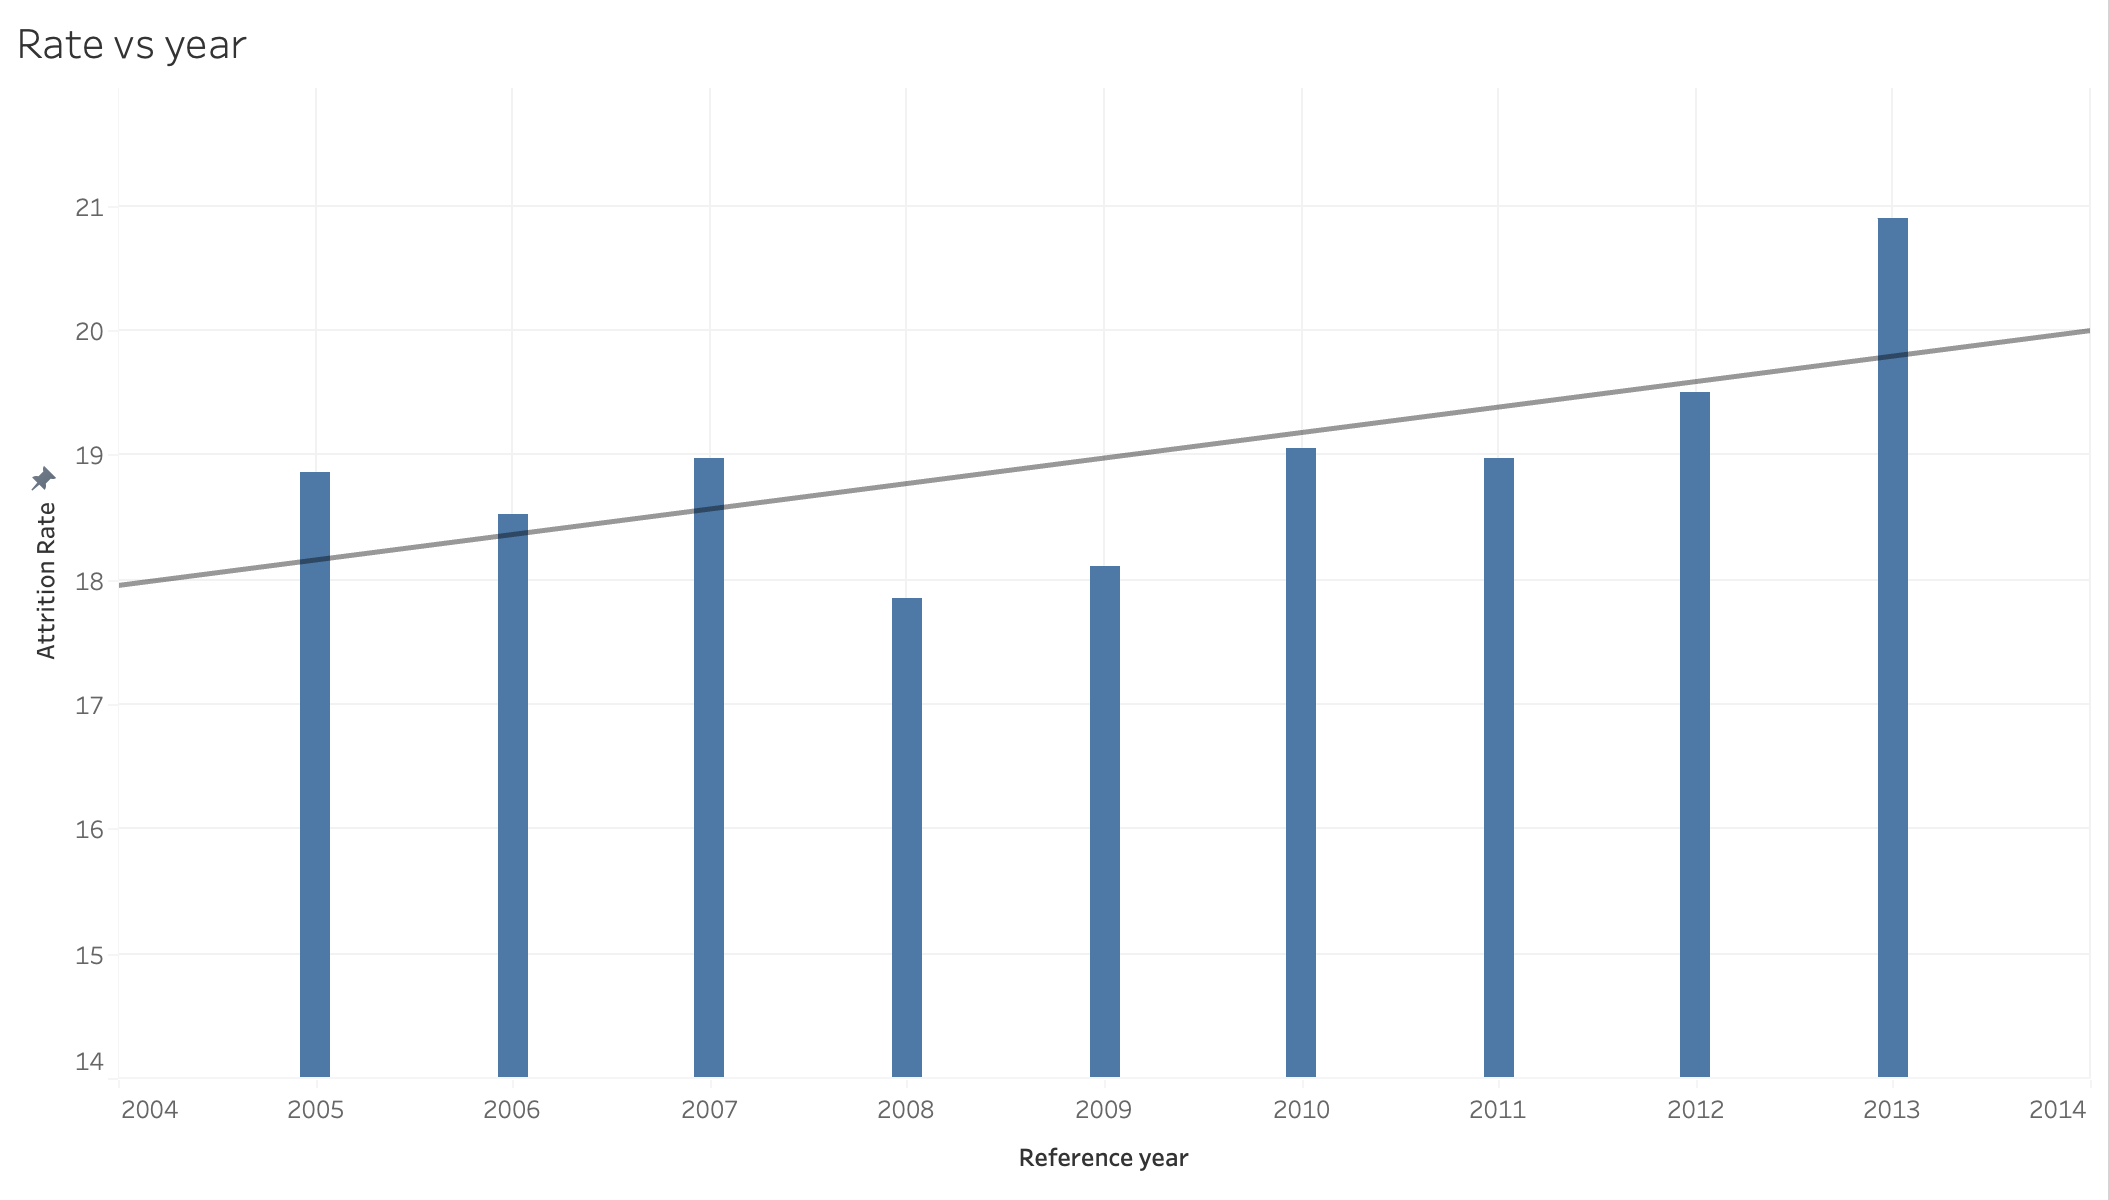
\includegraphics[width=0.5\textwidth]{images/Fig 1.png}
    \caption{Bar plot between Attrition Rate(\%) and Year}
    \label{fig:bar1}
\end{figure}

\subsubsection{Overall attrtion rate across years}
One can observe from Figure \ref{fig:bar1}, a general increase in attrition rates each year, with an exception in 2008. \par Several factors contributed to this anomaly, including the Global Financial Crisis, which led more students to stay in education due to a challenging job market. Additionally, government reforms increased funding and support for higher education, enhanced student support services improved retention. A focus on education quality also helped engage students and reduce dropouts.

\subsubsection{Age Group Analysis}

An area graph showing attrition rate versus year for different age groups is plotted in Figure \ref{fig:area1}. This graph reveals that the trends for individual age groups align closely with the overall attrition rate.

\begin{figure}[H]
    \centering
    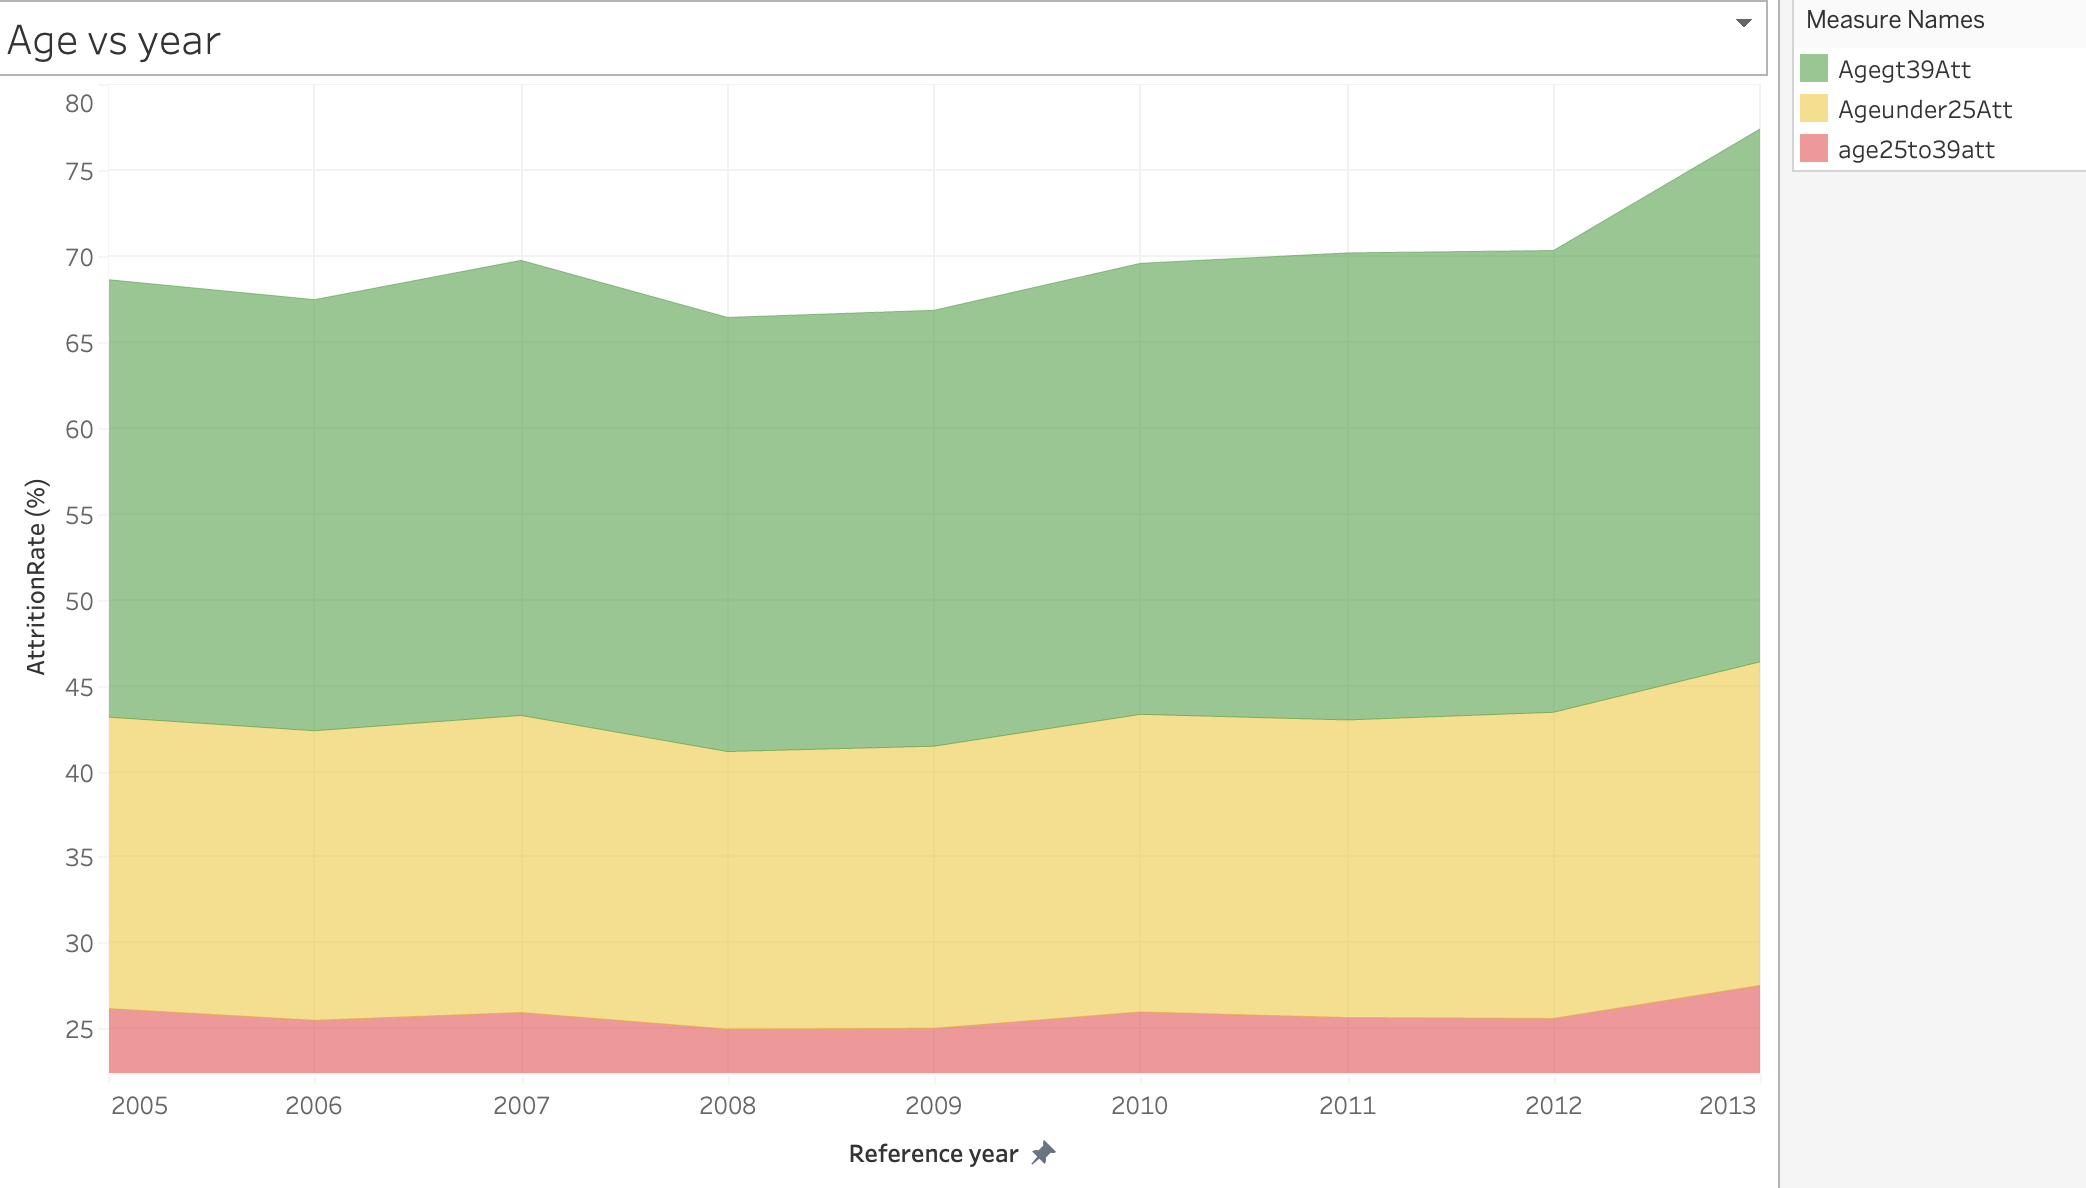
\includegraphics[width=0.4\textwidth]{images/Fig2.png}
    \caption{Area plot showing attrition rate (\%) by year for different age groups}
    \label{fig:area1}
\end{figure}

Key observations from this plot include:
\begin{itemize}
    \item The 25 to 39 years age group has the lowest attrition rate, likely due to greater stability in personal and professional lives.
    \item The age group above 39 years consistently shows the highest attrition rate, possibly due to increased job responsibilities, financial pressures, and personal commitments.
    \item The age group below 25 years shows moderate attrition rates, younger students might be more prone to dropping out due to the challenges of adjusting to higher education, exploring career paths, or switching courses.
\end{itemize}

\subsubsection{Gender-Based Analysis}
Figures \ref{fig:barline1} and \ref{fig:pie1} present the gender-based analysis. Figure \ref{fig:barline1} displays a bar graph for males and a line graph for females, while Figure \ref{fig:pie1} shows a pie chart of the average attrition rate by gender.

\begin{figure}[H]
    \centering
    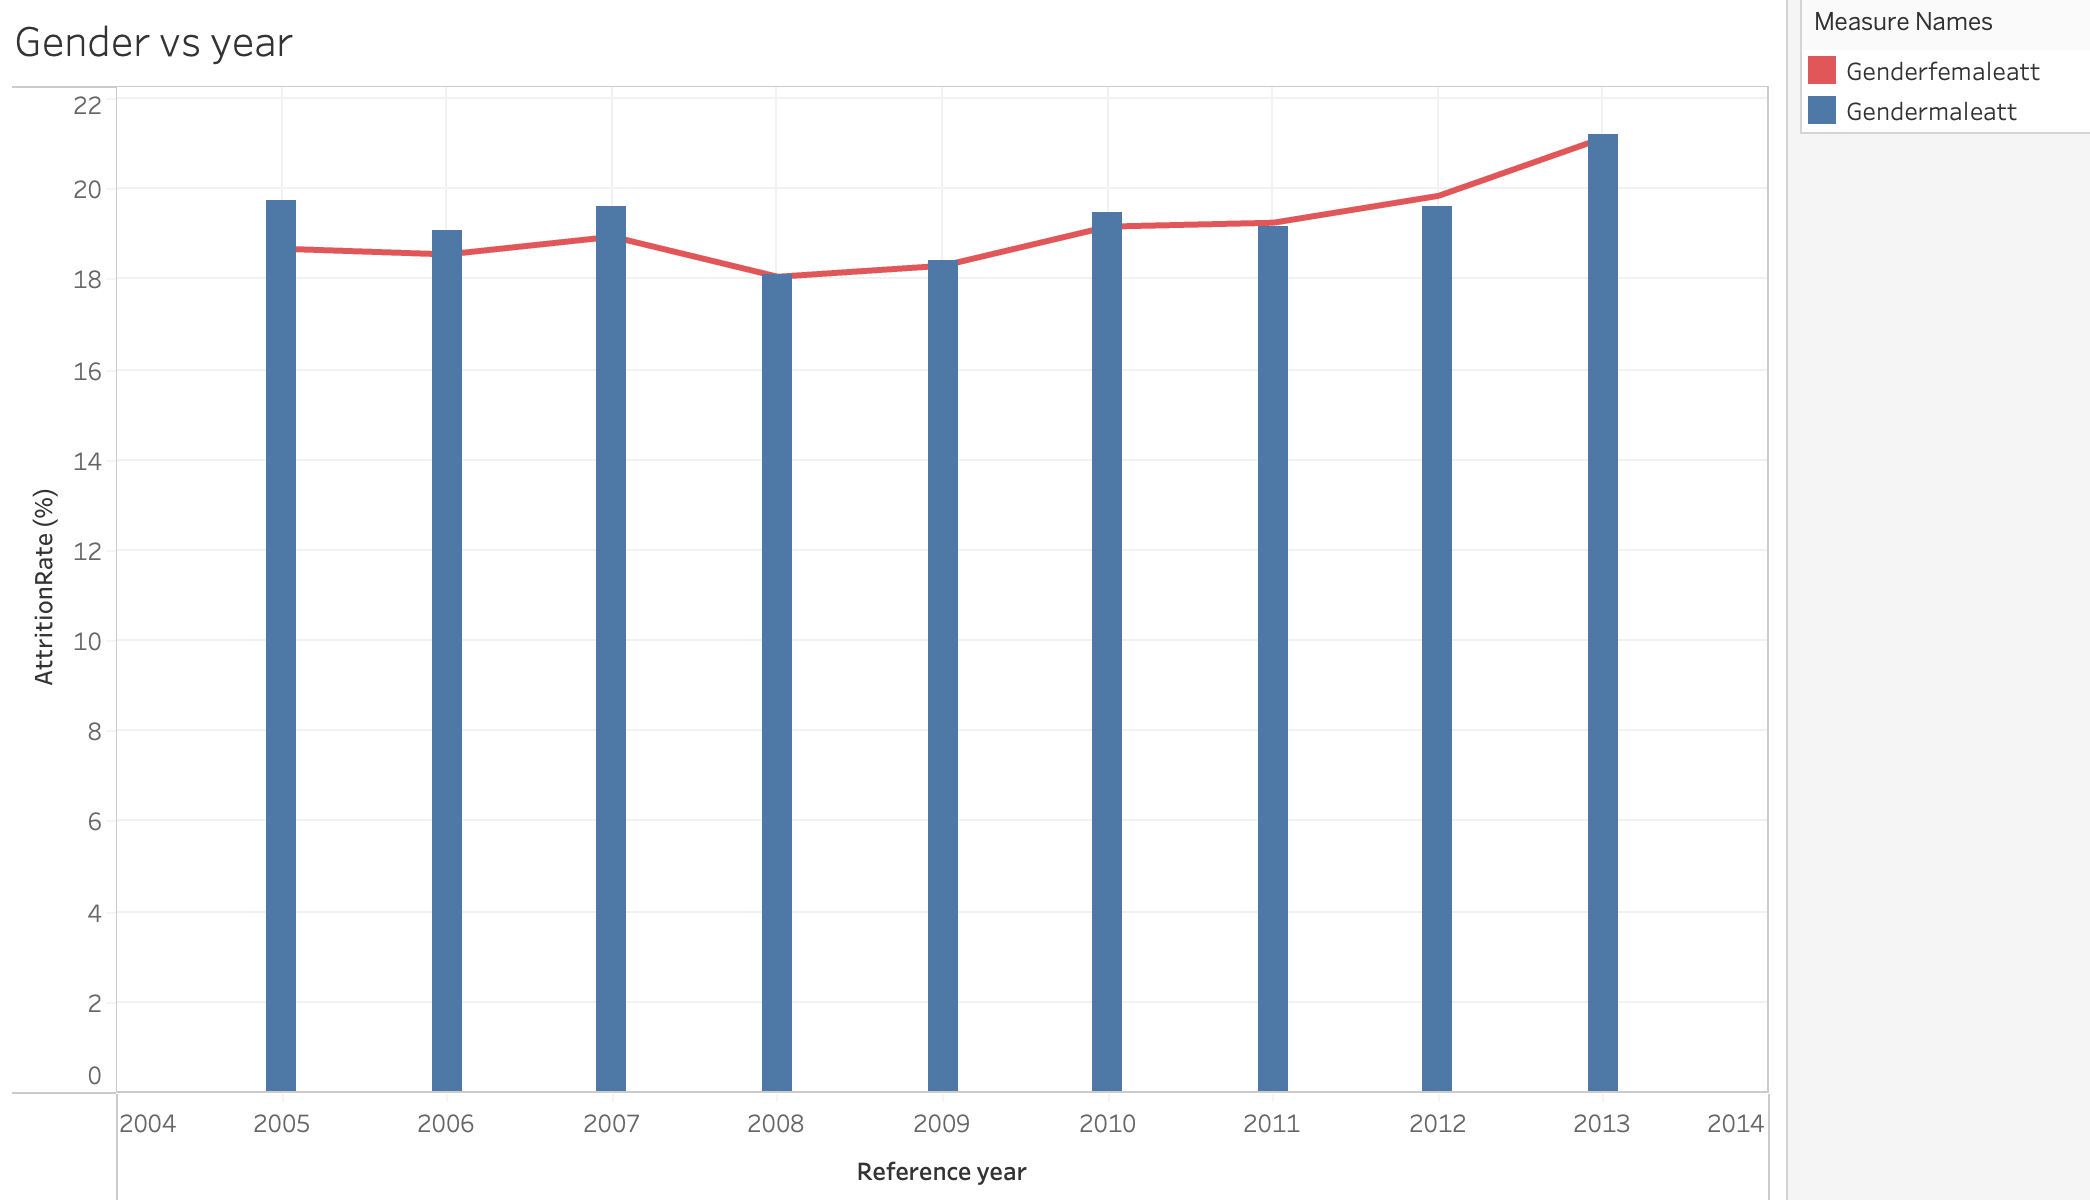
\includegraphics[width=0.4\textwidth]{images/Fig3.png}
    \caption{Bar and line plot of attrition rate by gender (male: bar, female: line) over time}
    \label{fig:barline1}
\end{figure}

\begin{figure}[H]
    \centering
    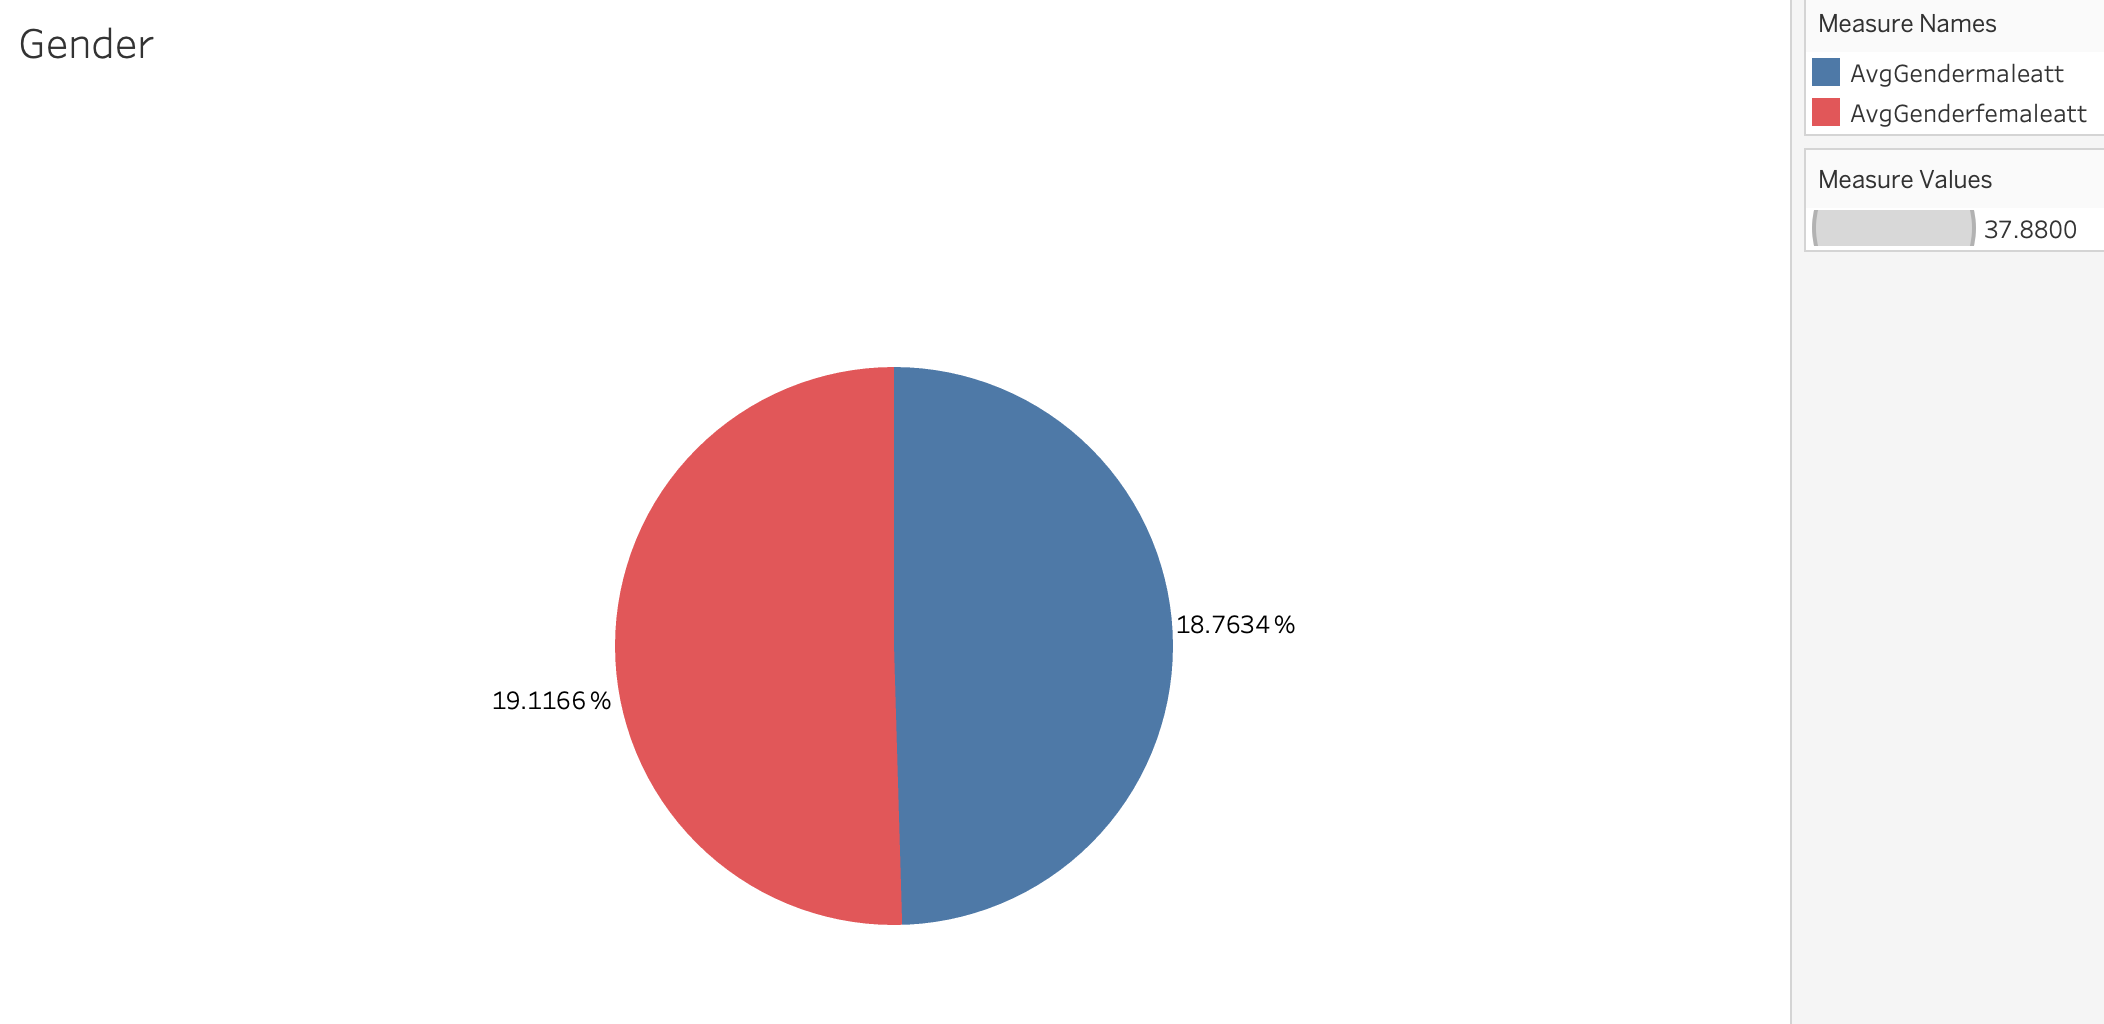
\includegraphics[width=0.4\textwidth]{images/Fig16.png}
    \caption{Pie chart of average attrition rate by gender}
    \label{fig:pie1}
\end{figure}

From these plots, the following key observations are made:
\begin{itemize}
    \item The combination of the line and bar plot in Figure \ref{fig:barline1} is used to compare attrition rates between genders.
    \item The pie chart in Figure \ref{fig:pie1} illustrates the overall attrition rate for males and females.
    \item The colors in Figures \ref{fig:barline1} and \ref{fig:pie1} are consistent, dark pink is used for female to highlight femininity and contrast with blue, while blue represents male for its common association with masculinity and clear differentiation..
    \item Figure \ref{fig:pie1} indicates that females have a higher overall attrition rate compared to males.
    \item Figure \ref{fig:barline1} shows that between 2005 and 2007, males had a higher attrition rate than females. However, from 2008 to 2013, the attrition rates for both genders were similar.
\end{itemize}

\textbf{Summary:} The analysis shows that females have a higher overall attrition rate compared to males, as seen in Figure \ref{fig:pie1}. From 2005 to 2007, female attrition was lower than male, but by 2008-2013, the rates were similar, suggesting that institutional changes may have addressed earlier challenges. The visualizations effectively highlight these trends and gender differences.


\subsubsection{Mode of Study Analysis}
A line graph depicting the average attrition rate across years for different modes of study is shown in Figure \ref{fig:line1}. Additionally, Figure \ref{fig:bar2} presents a horizontal bar graph of average attrition rates from 2005-2013 for these modes.

\begin{figure}[H]
    \centering
    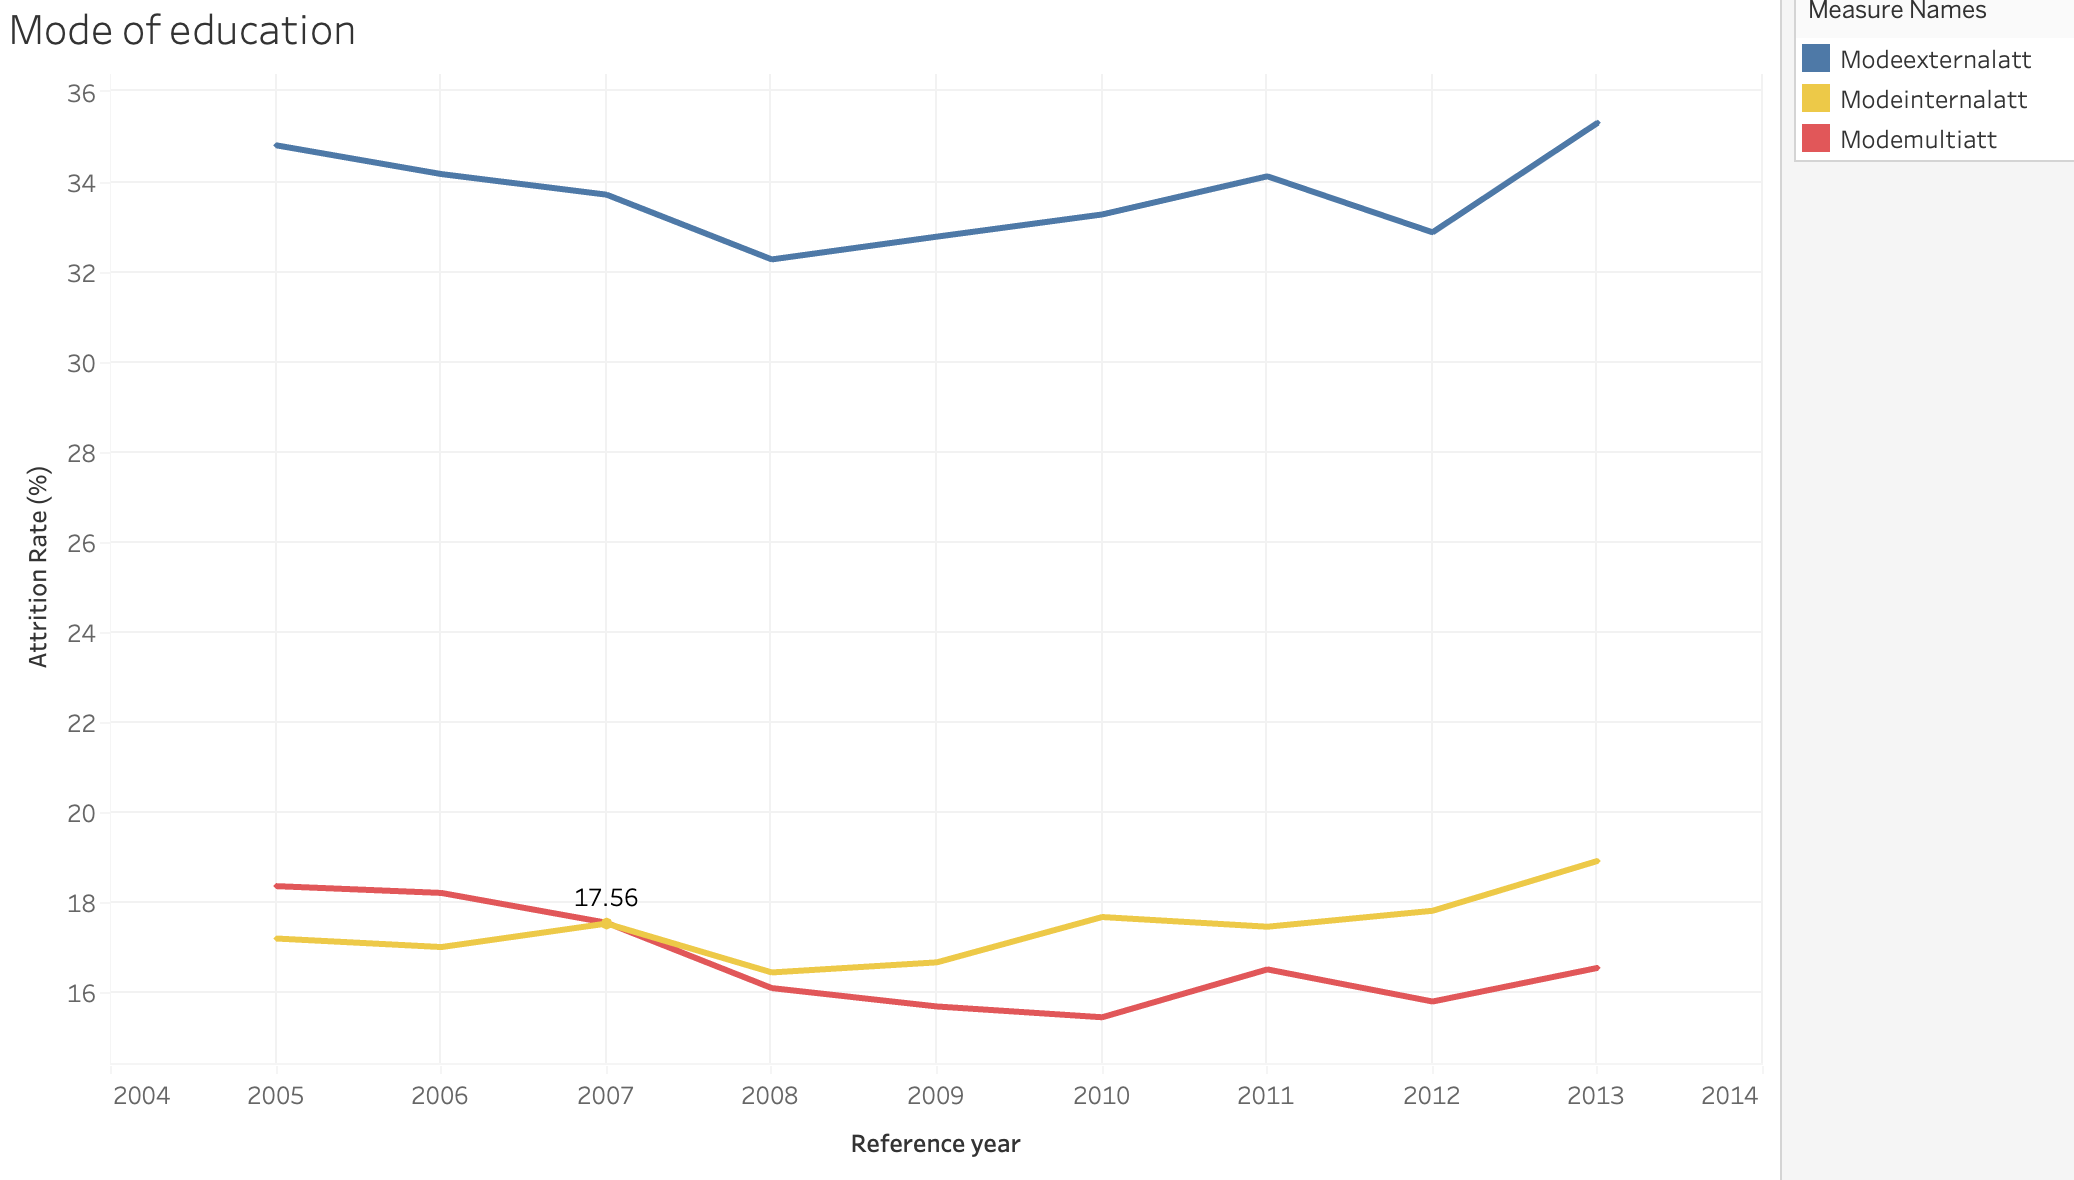
\includegraphics[width=0.4\textwidth]{images/Fig4.png}
    \caption{Line graph of average attrition rate across years for different modes of study}
    \label{fig:line1}    
\end{figure}

\begin{figure}[H]
    \centering
    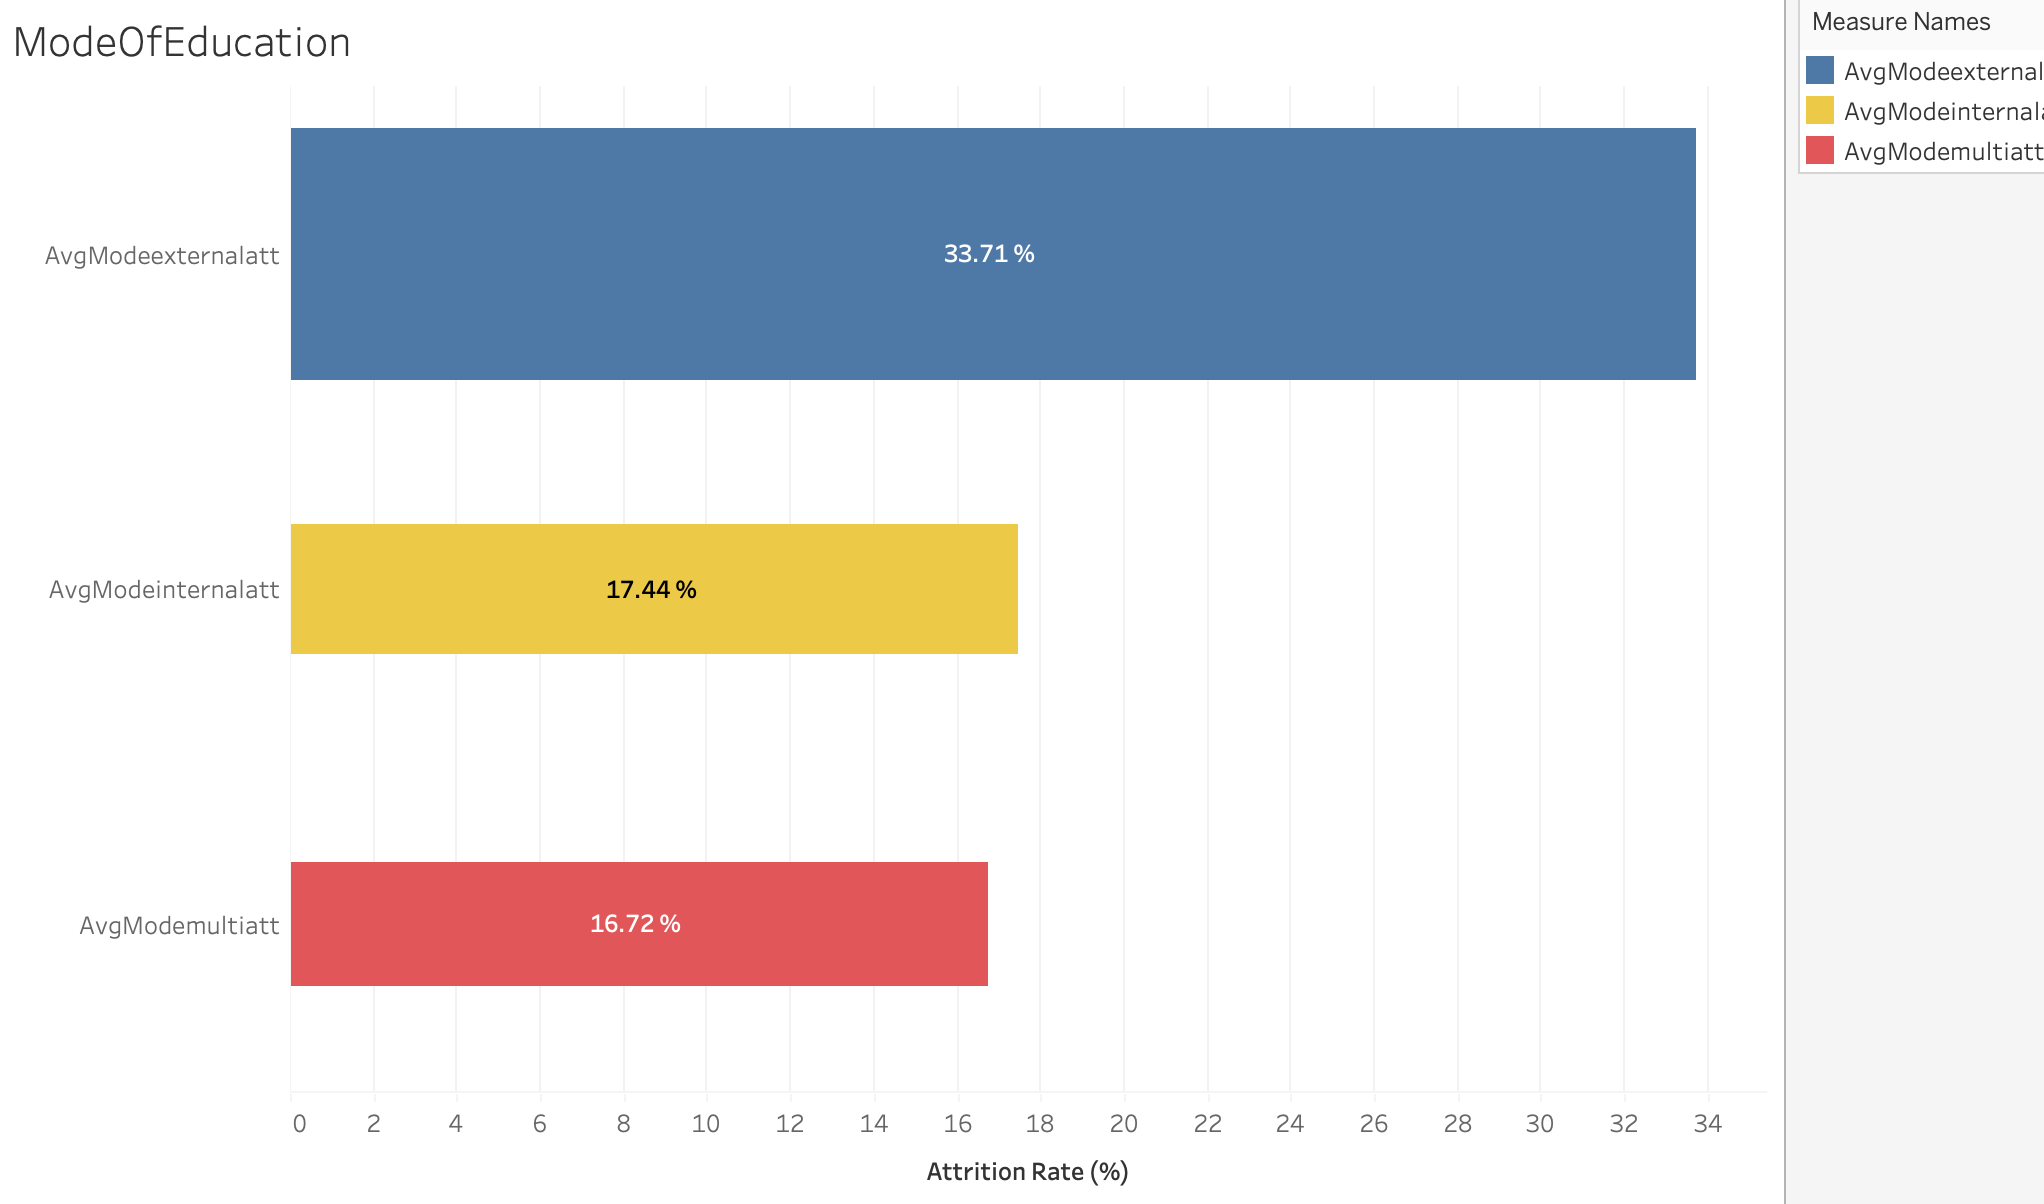
\includegraphics[width=0.4\textwidth]{images/Fig14.png}
    \caption{Horizontal bar graph of average attrition rate (2005-2013) for different modes of study}
    \label{fig:bar2}    
\end{figure}

From these plots, the following key observations are made:
\begin{itemize} 
    \item Figure \ref{fig:bar2} shows that external mode(blue) has the highest average attrition rate, followed by internal(yellow) and multi-mode(red) studies.
    \item The external mode's higher attrition rate is due to reduced support, interaction, and difficulties managing distractions and technology issues.
    \item Figure \ref{fig:line1} shows that before 2007, multi-mode study had higher attrition compared to internal mode, likely due to the complexities of hybrid formats and technology-related challenges.
    \item After 2007, Figure \ref{fig:line1} indicates that internal mode had higher attrition, possibly due to increased pressures or changes in delivery and support systems.
\end{itemize}

\textbf{Summary:} External modes lead to higher attrition rates due to distractions and technology issues. In contrast, multi-mode studies show lower attrition rates due to better engagement with technology and resources.

\subsubsection{Studying Full-Time and Part-Time Analysis}
Figures \ref{fig:line2} and \ref{fig:pie2} illustrate the attrition rates for full-time and part-time students. Figure \ref{fig:line2} presents a line graph showing attrition trends over the years, while Figure \ref{fig:pie2} provides a pie chart of average attrition rates from 2005-2013.

\begin{figure}[H]
    \centering
    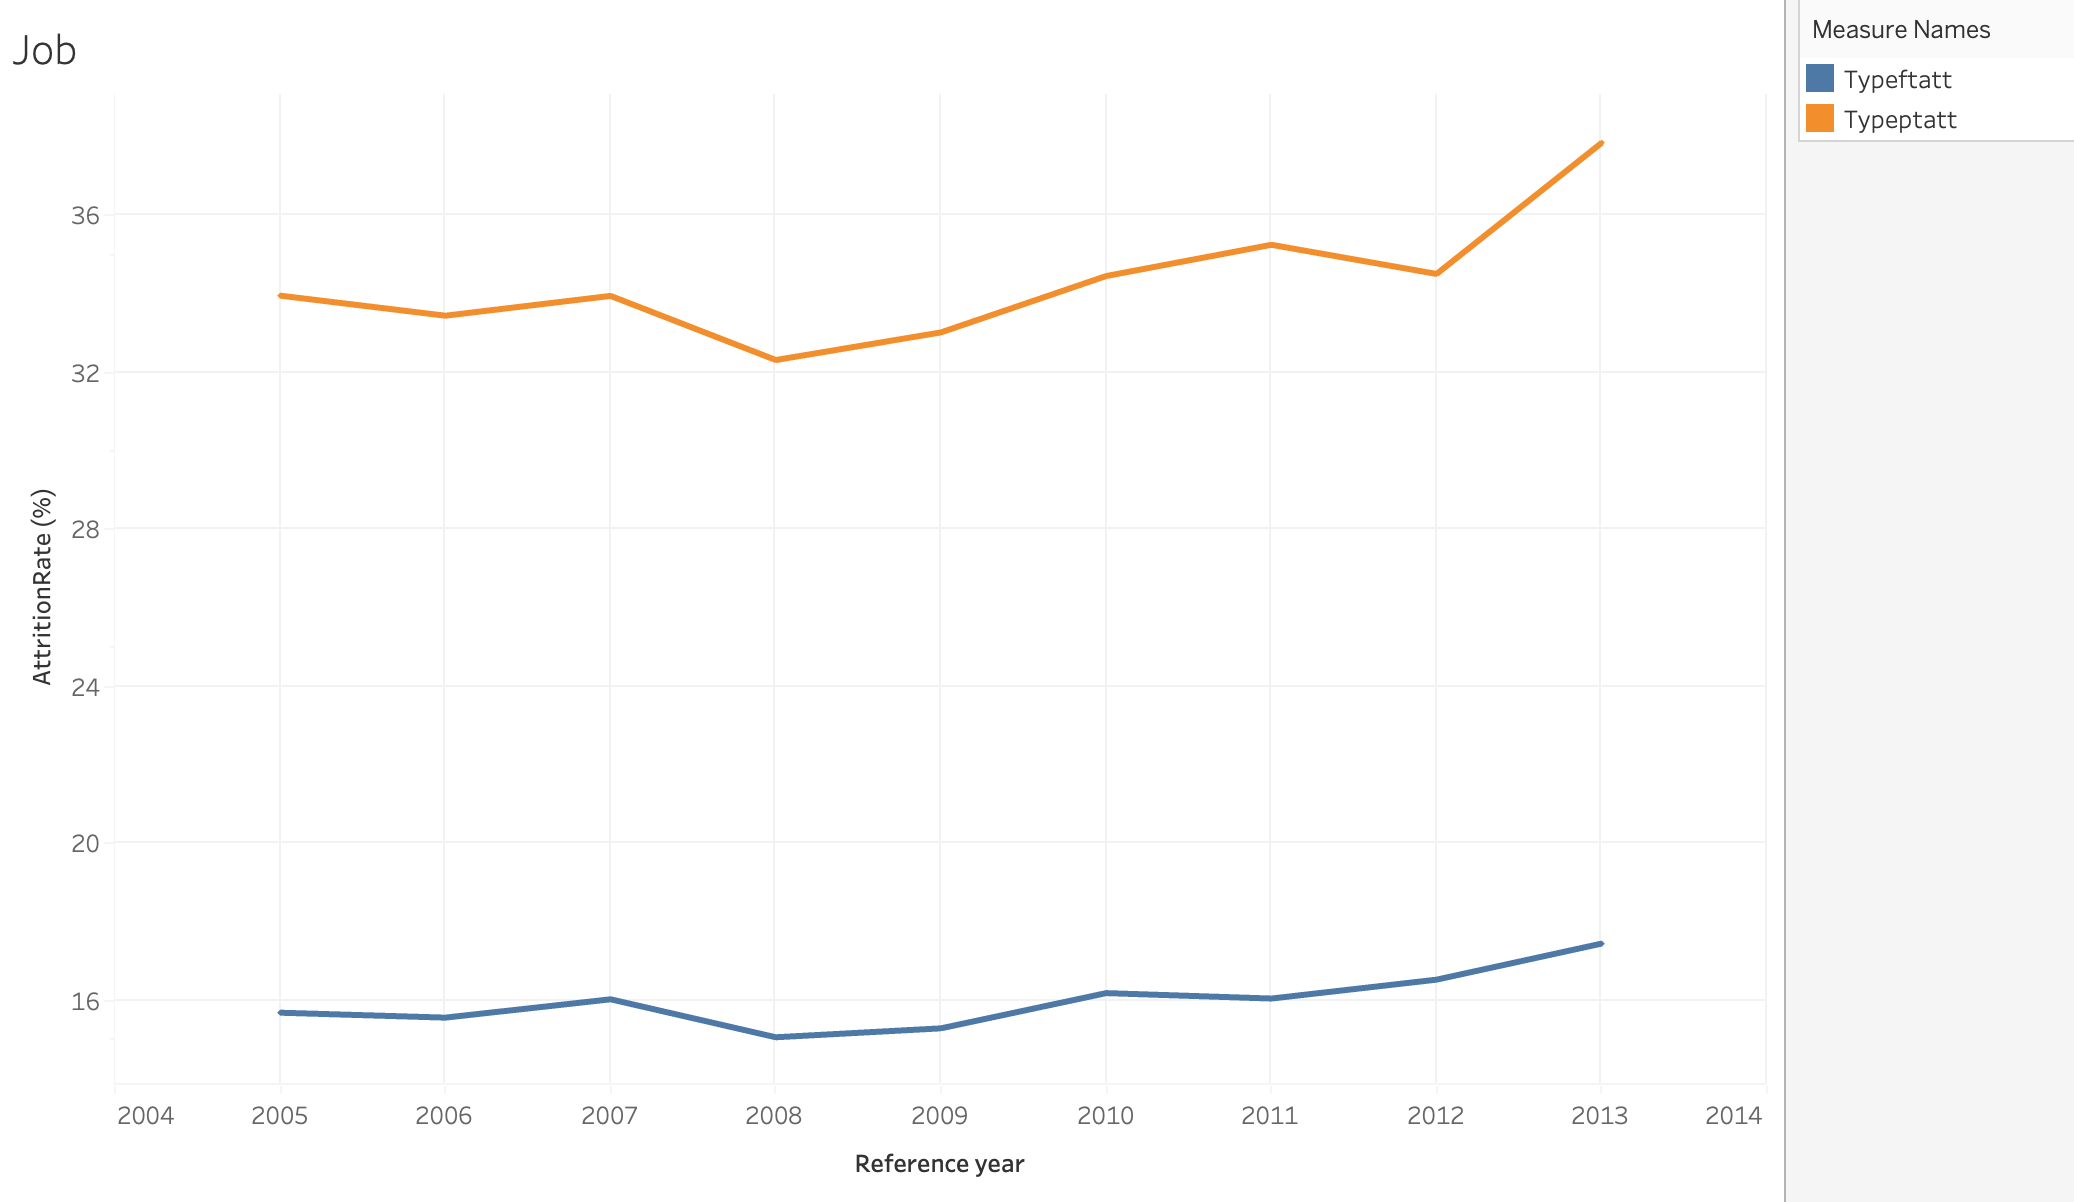
\includegraphics[width=0.4\textwidth]{images/Fig5.png}
    \caption{Line graph of attrition rate across years for full-time and part-time students}
    \label{fig:line2}    
\end{figure}

\begin{figure}[H]
    \centering
    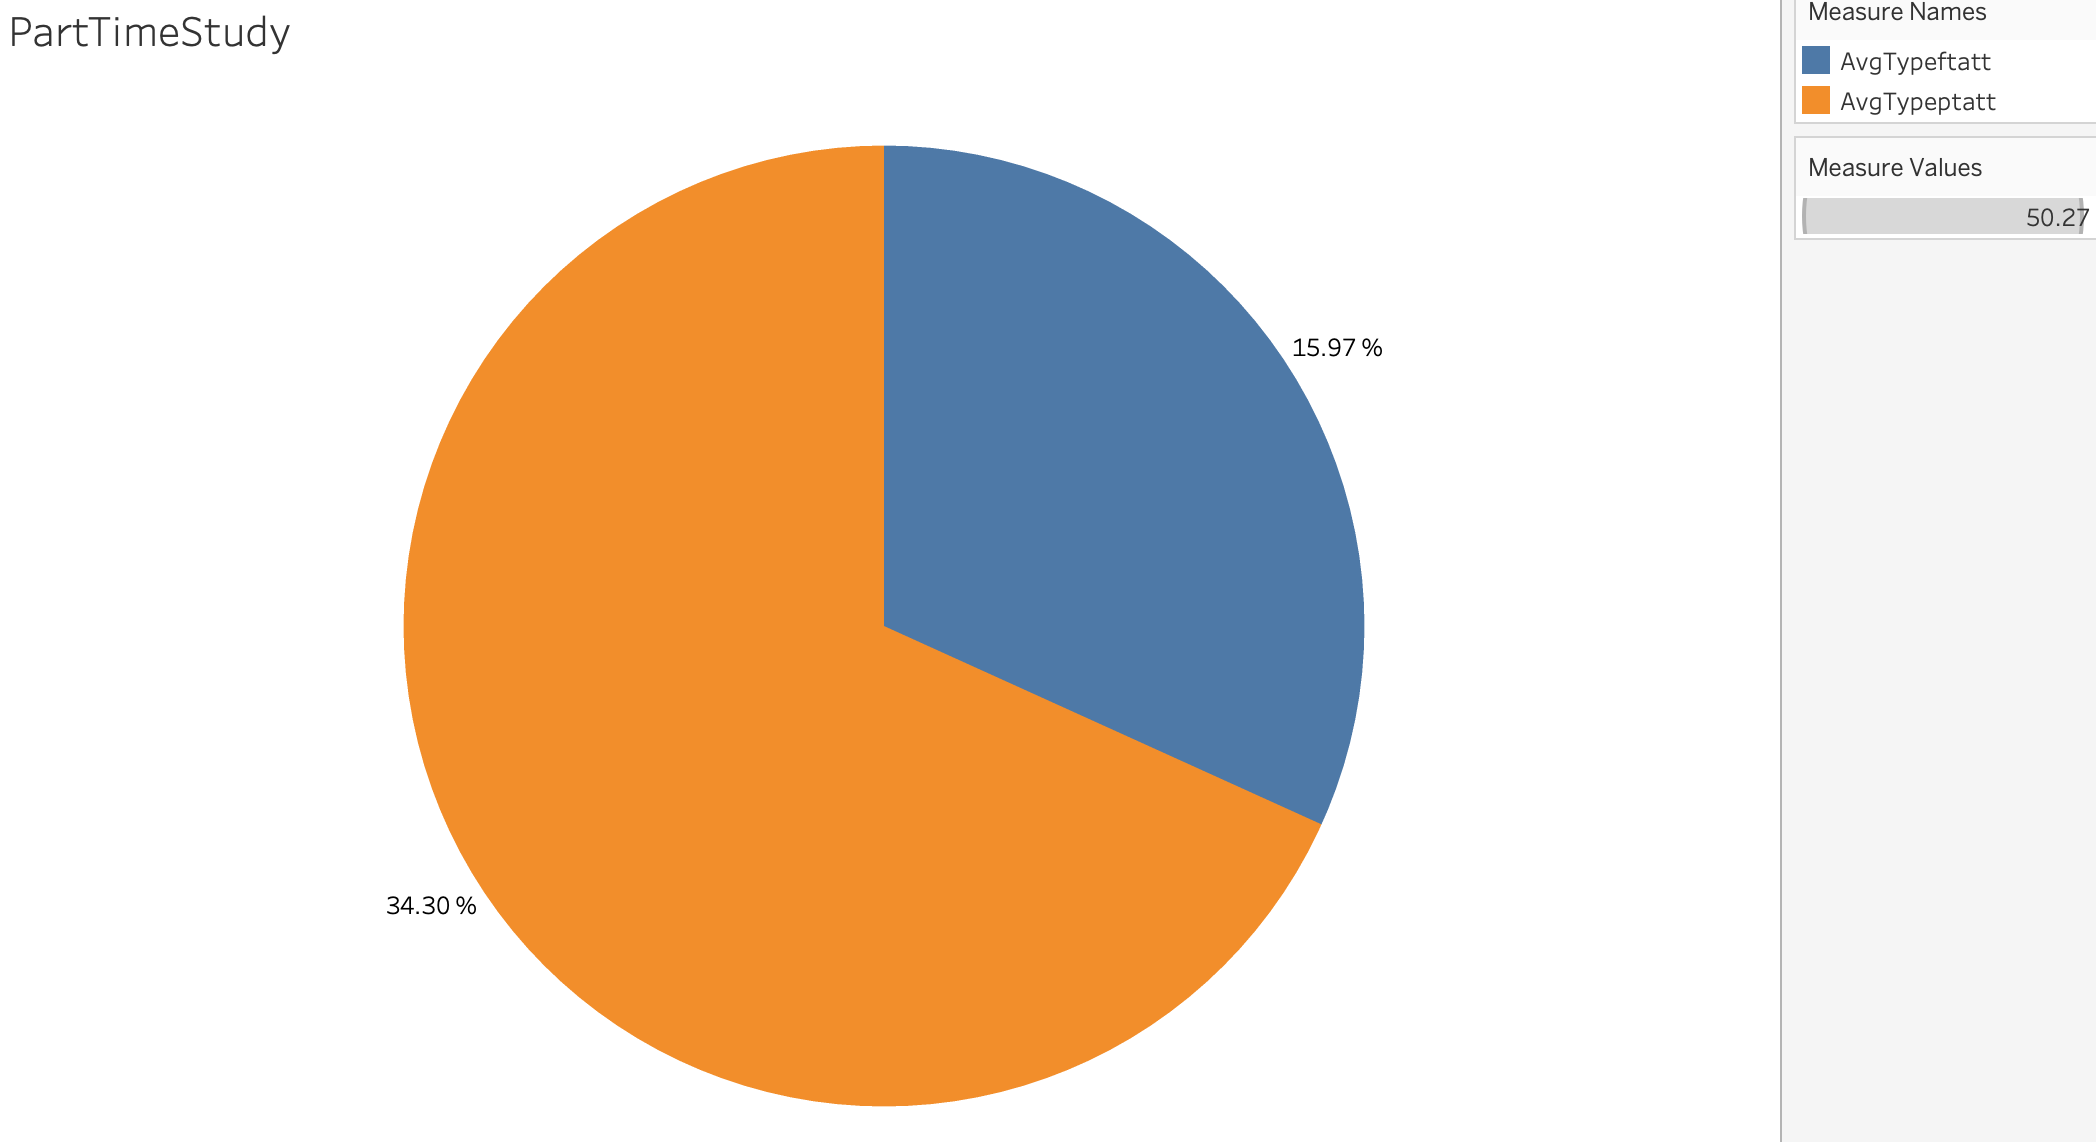
\includegraphics[width=0.4\textwidth]{images/Fig15.png}
    \caption{Pie chart of average attrition rate (2005-2013) for full-time and part-time students}
    \label{fig:pie2}    
\end{figure}

From these plots, the following key observations are made:
\begin{itemize} 
    \item Figures \ref{fig:line2} and \ref{fig:pie2} show that part-time students have a higher attrition rate compared to full-time students.
    \item Figure \ref{fig:pie2} highlights the proportion of attrition rates attributed to part-time versus full-time study.
    \item The higher attrition for part-time students may result from balancing work and study, reduced access to resources, and less academic engagement.
\end{itemize}

\textbf{Summary:} Part-time students have higher attrition rates compared to full-time students due to challenges in managing studies with other commitments. The visualizations effectively highlight these differences and the impact of study mode on attrition.

\subsubsection{Socio-Economic Status Analysis}

Figures \ref{fig:barline2} and \ref{fig:squar1} depict attrition rates for students from low socio-economic backgrounds across 2005-2013. The data is based on the 2006 and 2011 Australian Bureau of Statistics' Socio-Economic Indexes for Areas (SEIFA).

\begin{figure}[H]
    \centering
    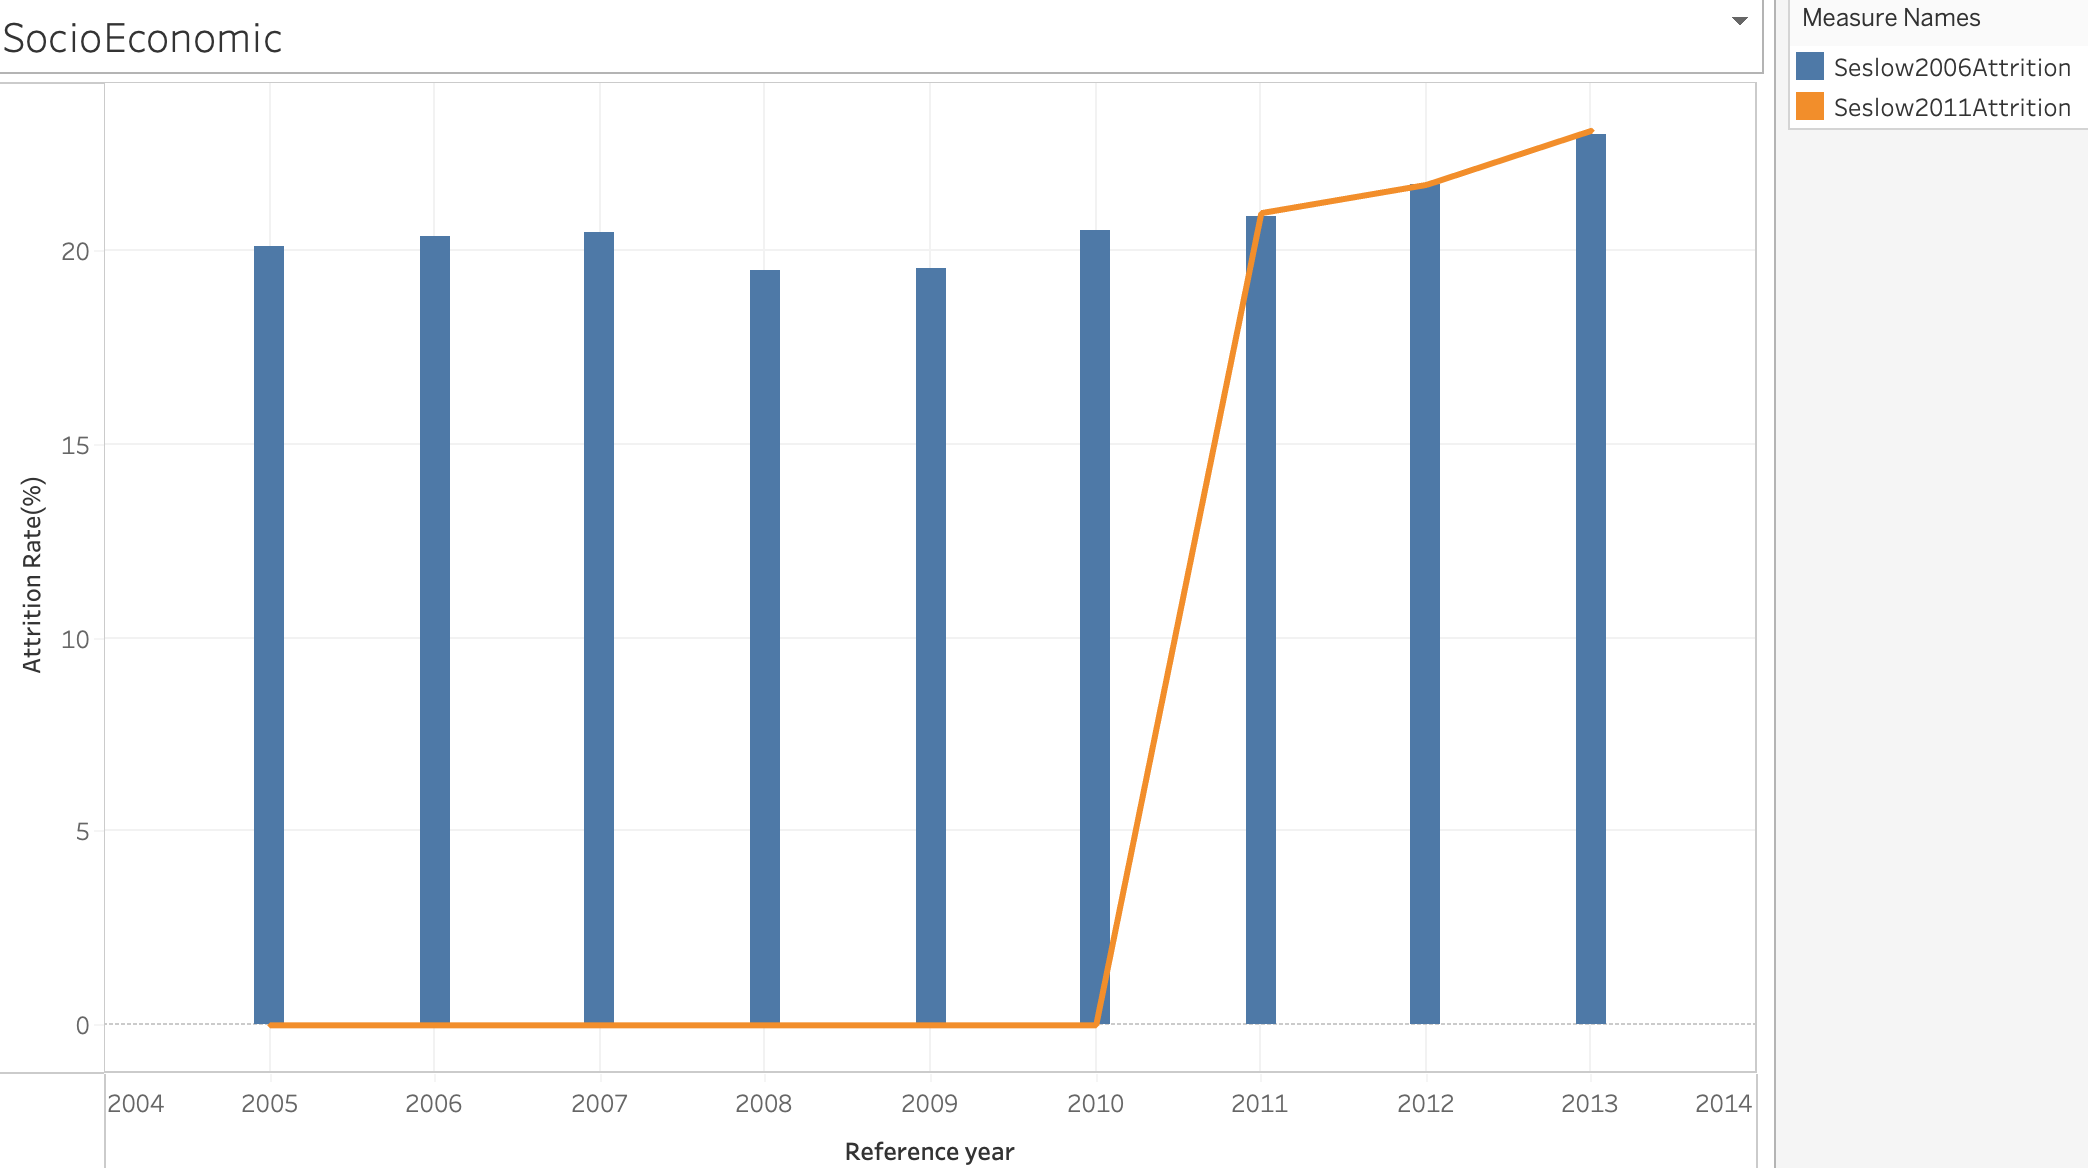
\includegraphics[width=0.4\textwidth]{images/Fig7.png}
    \caption{Attrition rate across years for low socio-economic background (2006 and 2011)}
    \label{fig:barline2}    
\end{figure}

\begin{figure}[H]
    \centering
    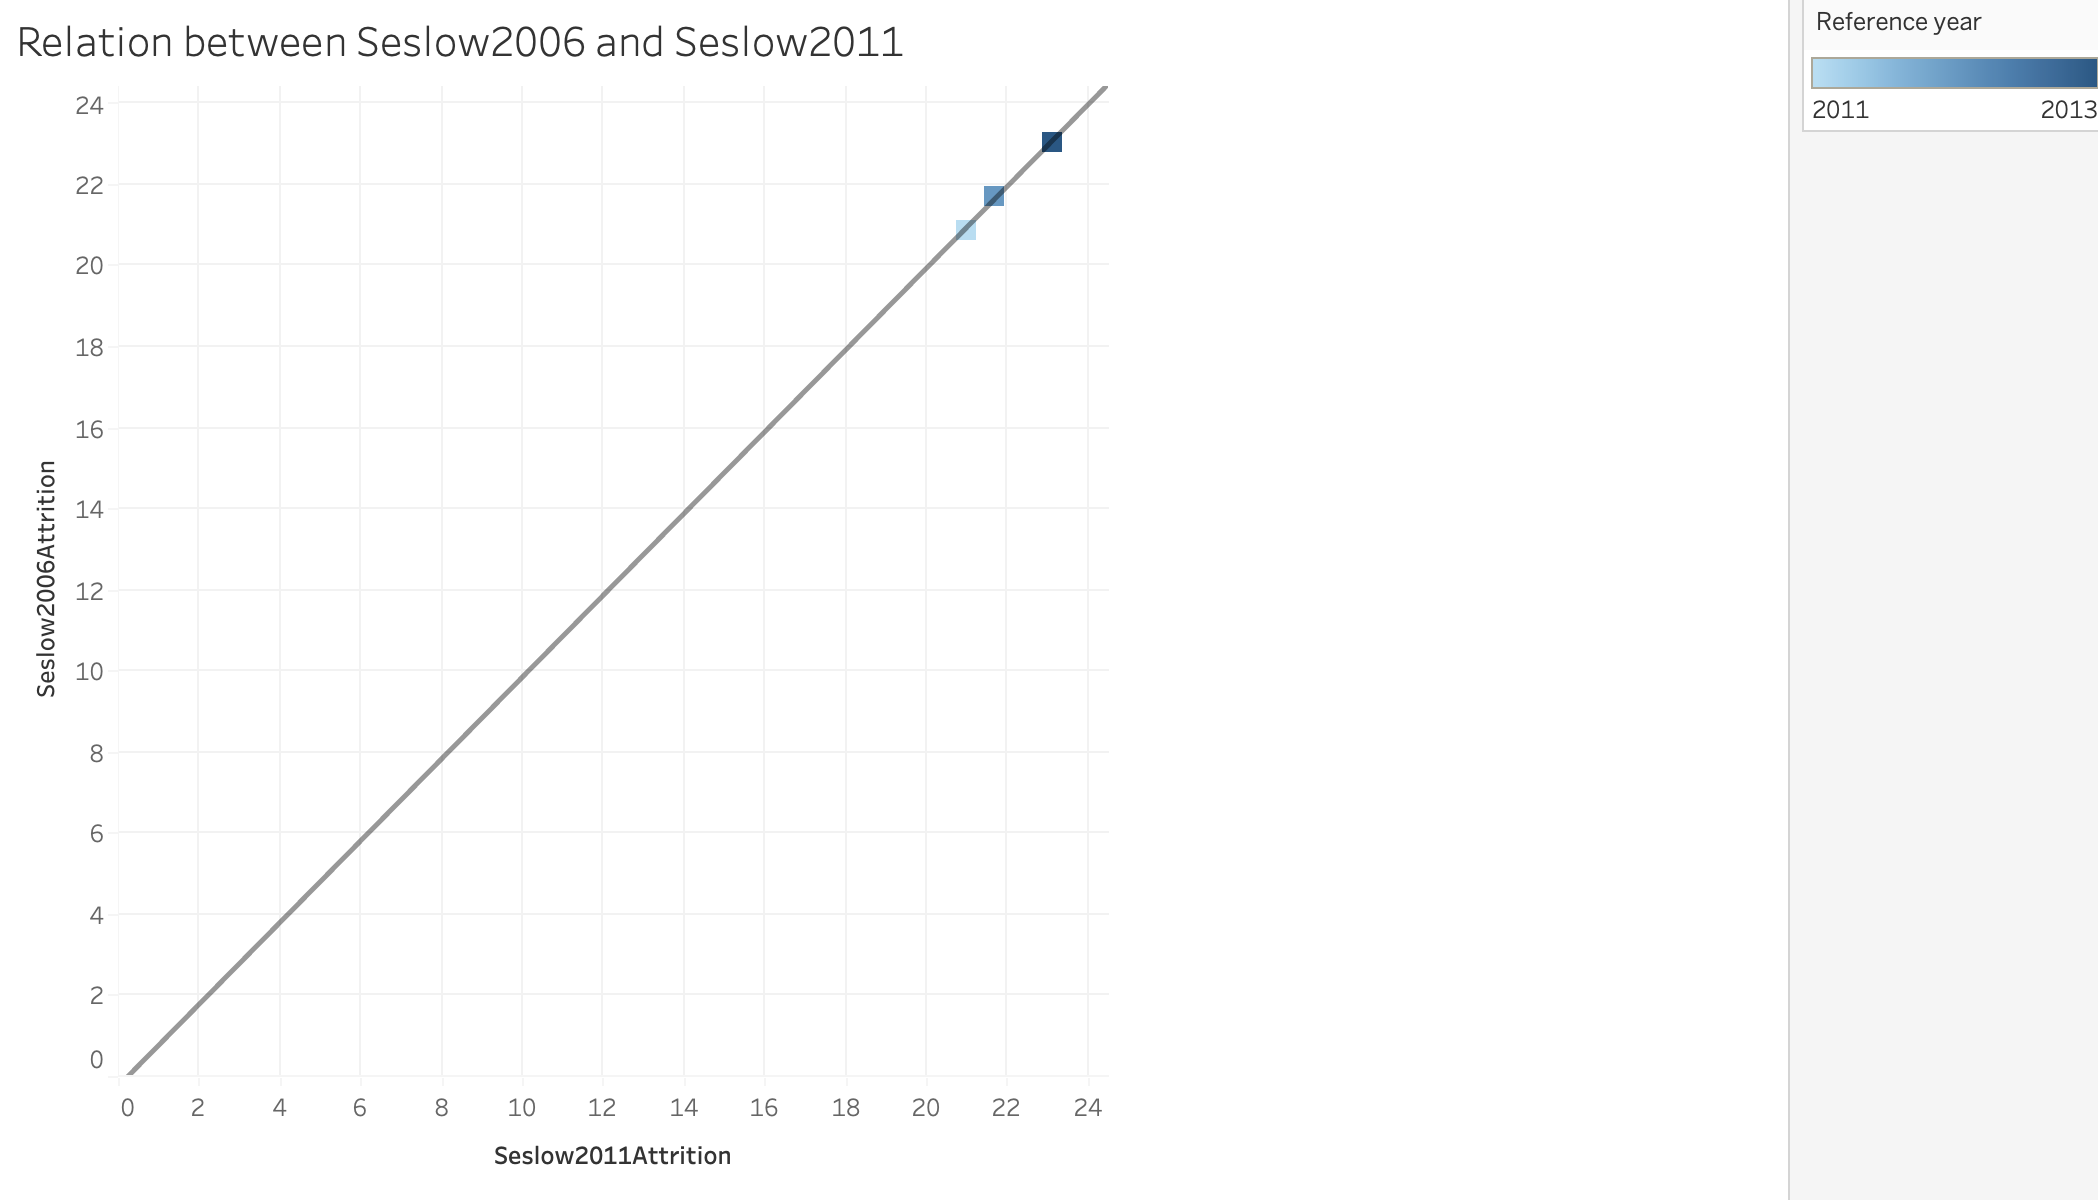
\includegraphics[width=0.4\textwidth]{images/Fig19.png}
    \caption{Comparison of low socio-economic background (2006 vs. 2011)}
    \label{fig:squar1}    
\end{figure}

\par \textit{Note:} Low socio-economic status is based on students’ postcode of permanent home residence mapped against the 2006 / 2011 Australian Bureau of Statistics' Socio-Economic Indexes for Areas (SEIFA) Index of Education and Occupation by postal area, with the postal areas containing the bottom 25\% of the population aged 15-64 on the SEIFA file being classified as low socio-economic

\par From these plots, the following key observations are made:
\begin{itemize} 
    \item Figure \ref{fig:barline2} shows similar attrition trends for low socio-economic backgrounds in 2006 and 2011, consistent with Figure \ref{fig:squar1}.
    \item Figure \ref{fig:barline2} reveals zero attrition for SESlow2011 between 2005-2010, since it's from 2011, while Figure \ref{fig:squar1} excludes these early data points in its analysis.
    \item The consistency between SESlow2006 and SESlow2011 suggests stable attrition patterns over the years for low socio-economic backgrounds.
    \item For the line chart representing 2011, orange is chosen to provide a vibrant and clear contrast to the blue, making it easy to distinguish between the two years
\end{itemize}

\textbf{Summary:} Attrition rates for students from low socio-economic backgrounds remain consistent between 2006 and 2011. The data indicates a stable relationship between these socio-economic indices over time.

\subsubsection{Non-English Speaking Students Analysis}

Figure \ref{fig:bar3} presents the attrition rates for non-English speaking students between 2005-2013.

\begin{figure}[H] 
    \centering 
    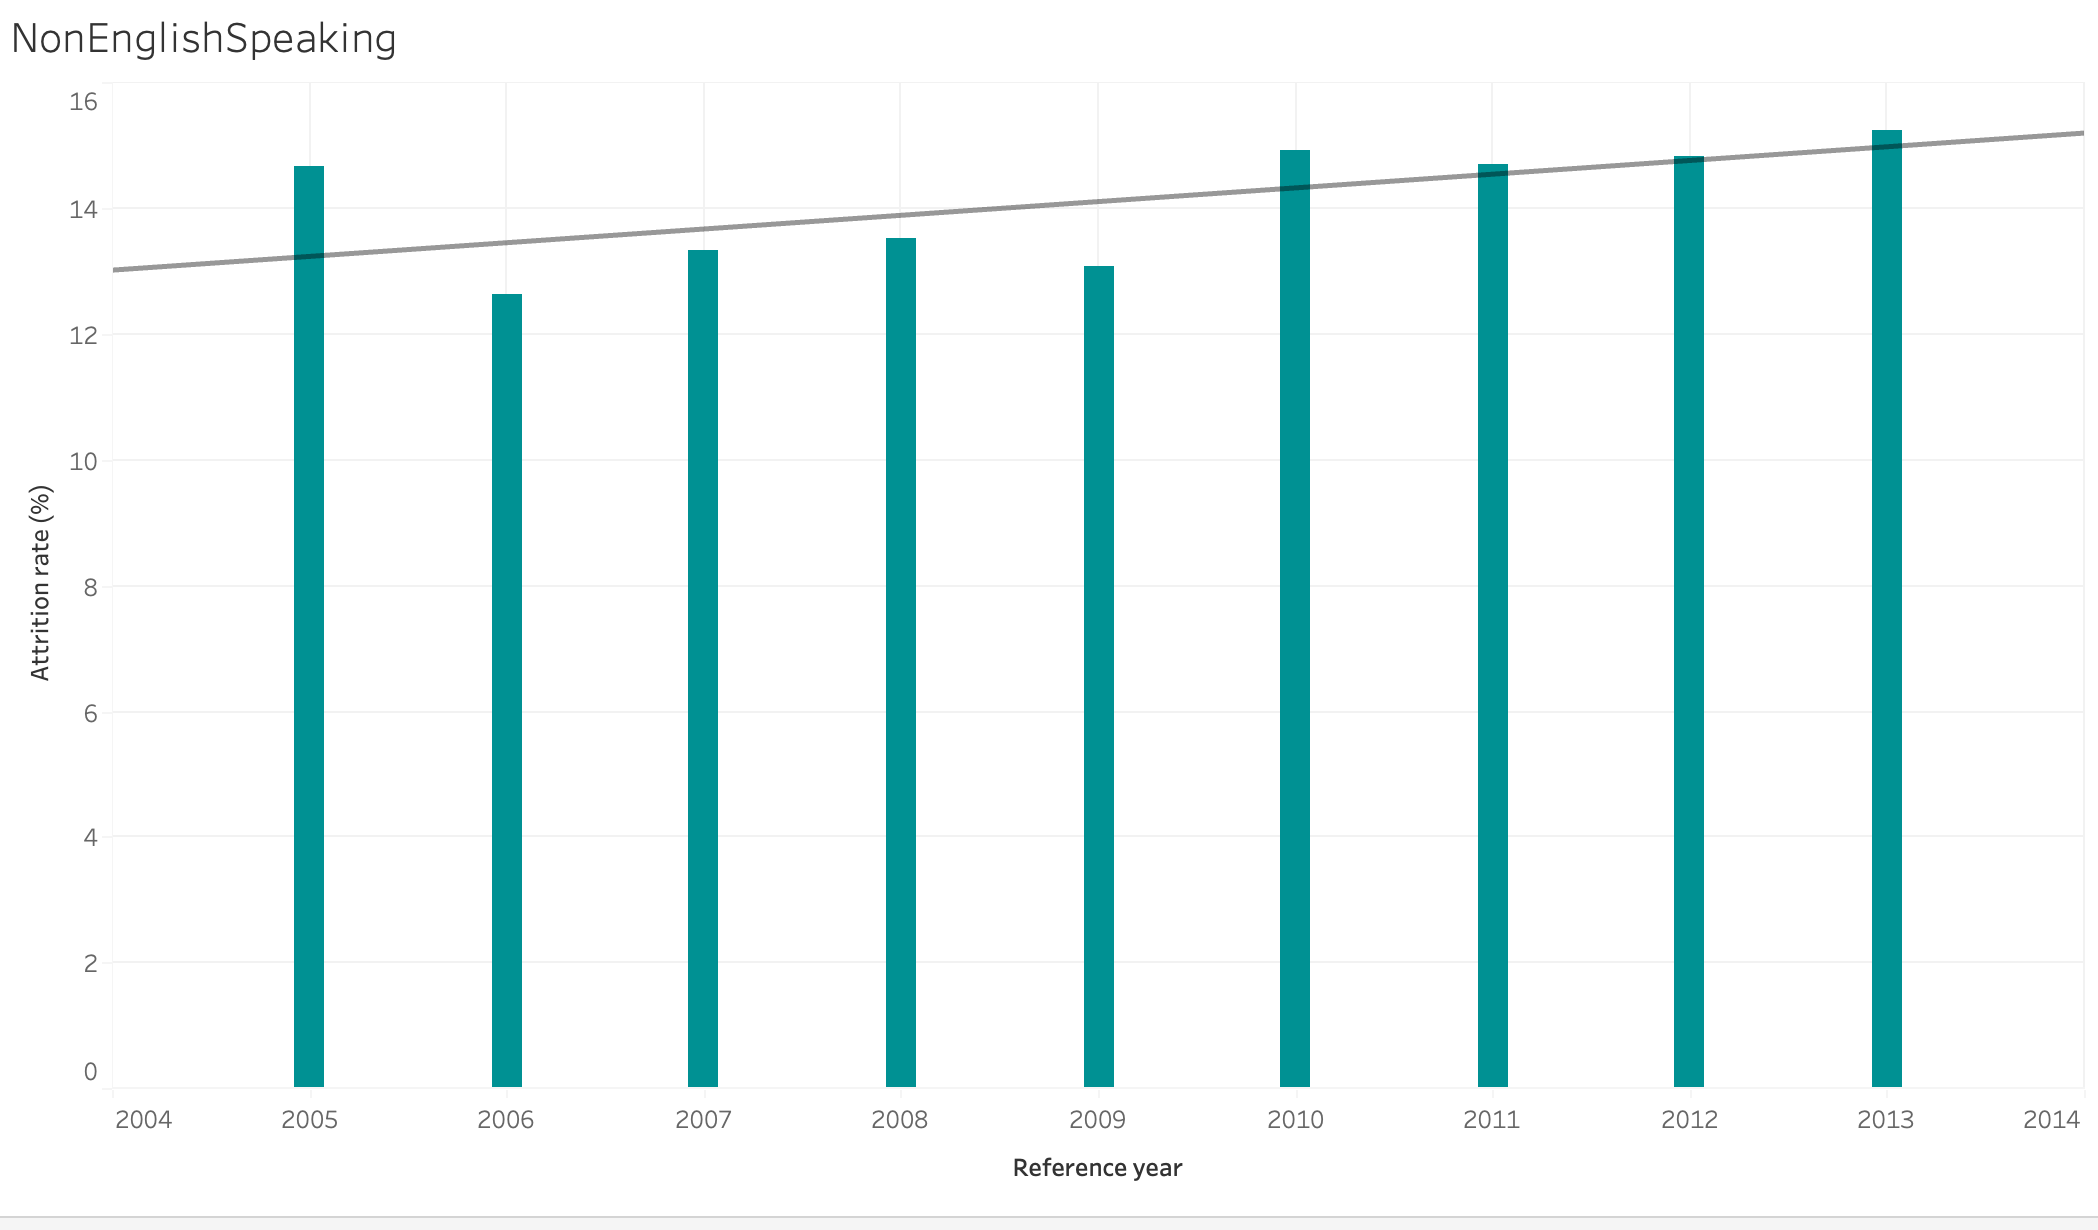
\includegraphics[width=0.4\textwidth]{images/Fig6.png} 
    \caption{Bar plot for attrition rate across years for non-English speaking students} 
    \label{fig:bar3}
\end{figure}

\par From the plot, the following key observations are made: \begin{itemize} 
    \item Figure \ref{fig:bar3} shows a slight but consistent increase in attrition rates for non-English speaking students over the years. \item The trend line in Figure \ref{fig:bar3} confirms this gradual rise. 
    \item Teal is selected as the color for this Figure \ref{fig:bar3} because it is often associated with inclusivity and communication, aligning with the theme of addressing challenges faced by non-English speaking students. This choice ensures the data is clearly conveyed and thoughtfully represented..

\end{itemize}

\textbf{Summary:} Attrition rates for non-English speaking students have steadily increased over time, possibly due to language barriers, cultural adjustments, or difficulties accessing support services in a primarily English-speaking environment.

\subsubsection{Disability of Students Analysis}

Figure \ref{fig:bar4} presents attrition rates for students with disabilities from 2005-2013.

\begin{figure}[H] 
    \centering 
    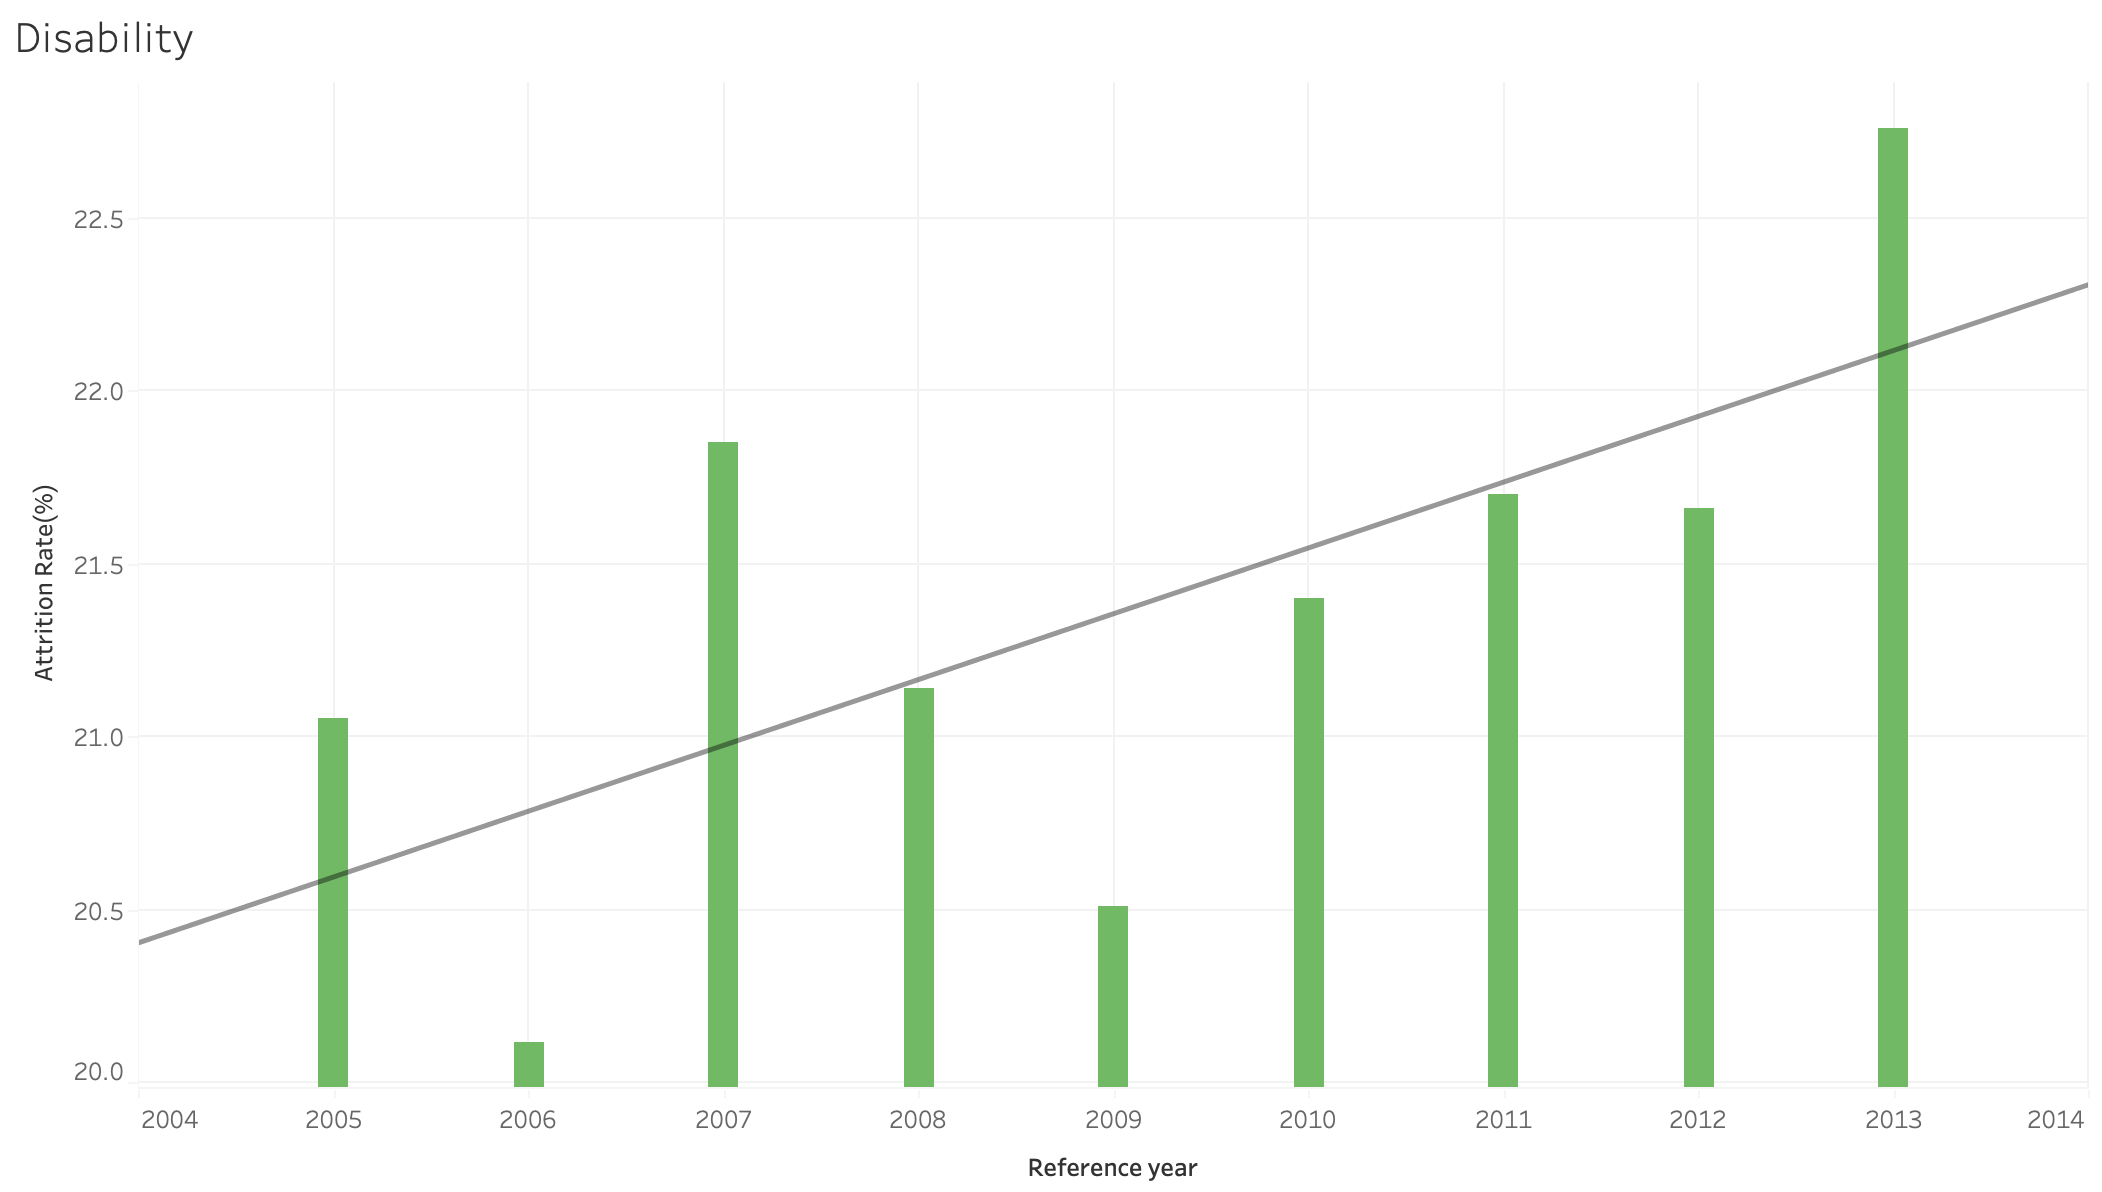
\includegraphics[width=0.4\textwidth]{images/Fig8.png} 
    \caption{Bar plot for attrition rate across years for students with disabilities} 
    \label{fig:bar4} 
\end{figure}

\par From the plot, the following key observations are made:  \begin{itemize}
    \item Attrition rates for students with disabilities gradually increased over the years, as shown in Figure \ref{fig:bar4}. 
    \item 2006 shows the lowest attrition rate, likely due to the 2005 Disability Standards for Education, which improved support and accessibility. 
    \item Green color is used in Figure \ref{fig:bar4} to represent the data for students with disabilities, symbolizing support and well-being.
\end{itemize}

\textbf{Summary:} Despite early improvements, attrition rates for students with disabilities have risen, possibly due to evolving challenges or insufficient ongoing support.


\subsubsection{Indigenous Students Analysis}

Figure \ref{fig:bar5} shows attrition rates for Indigenous students (Aboriginal and Torres Strait Islander) from 2005-2013.

\begin{figure}[H] 
    \centering 
    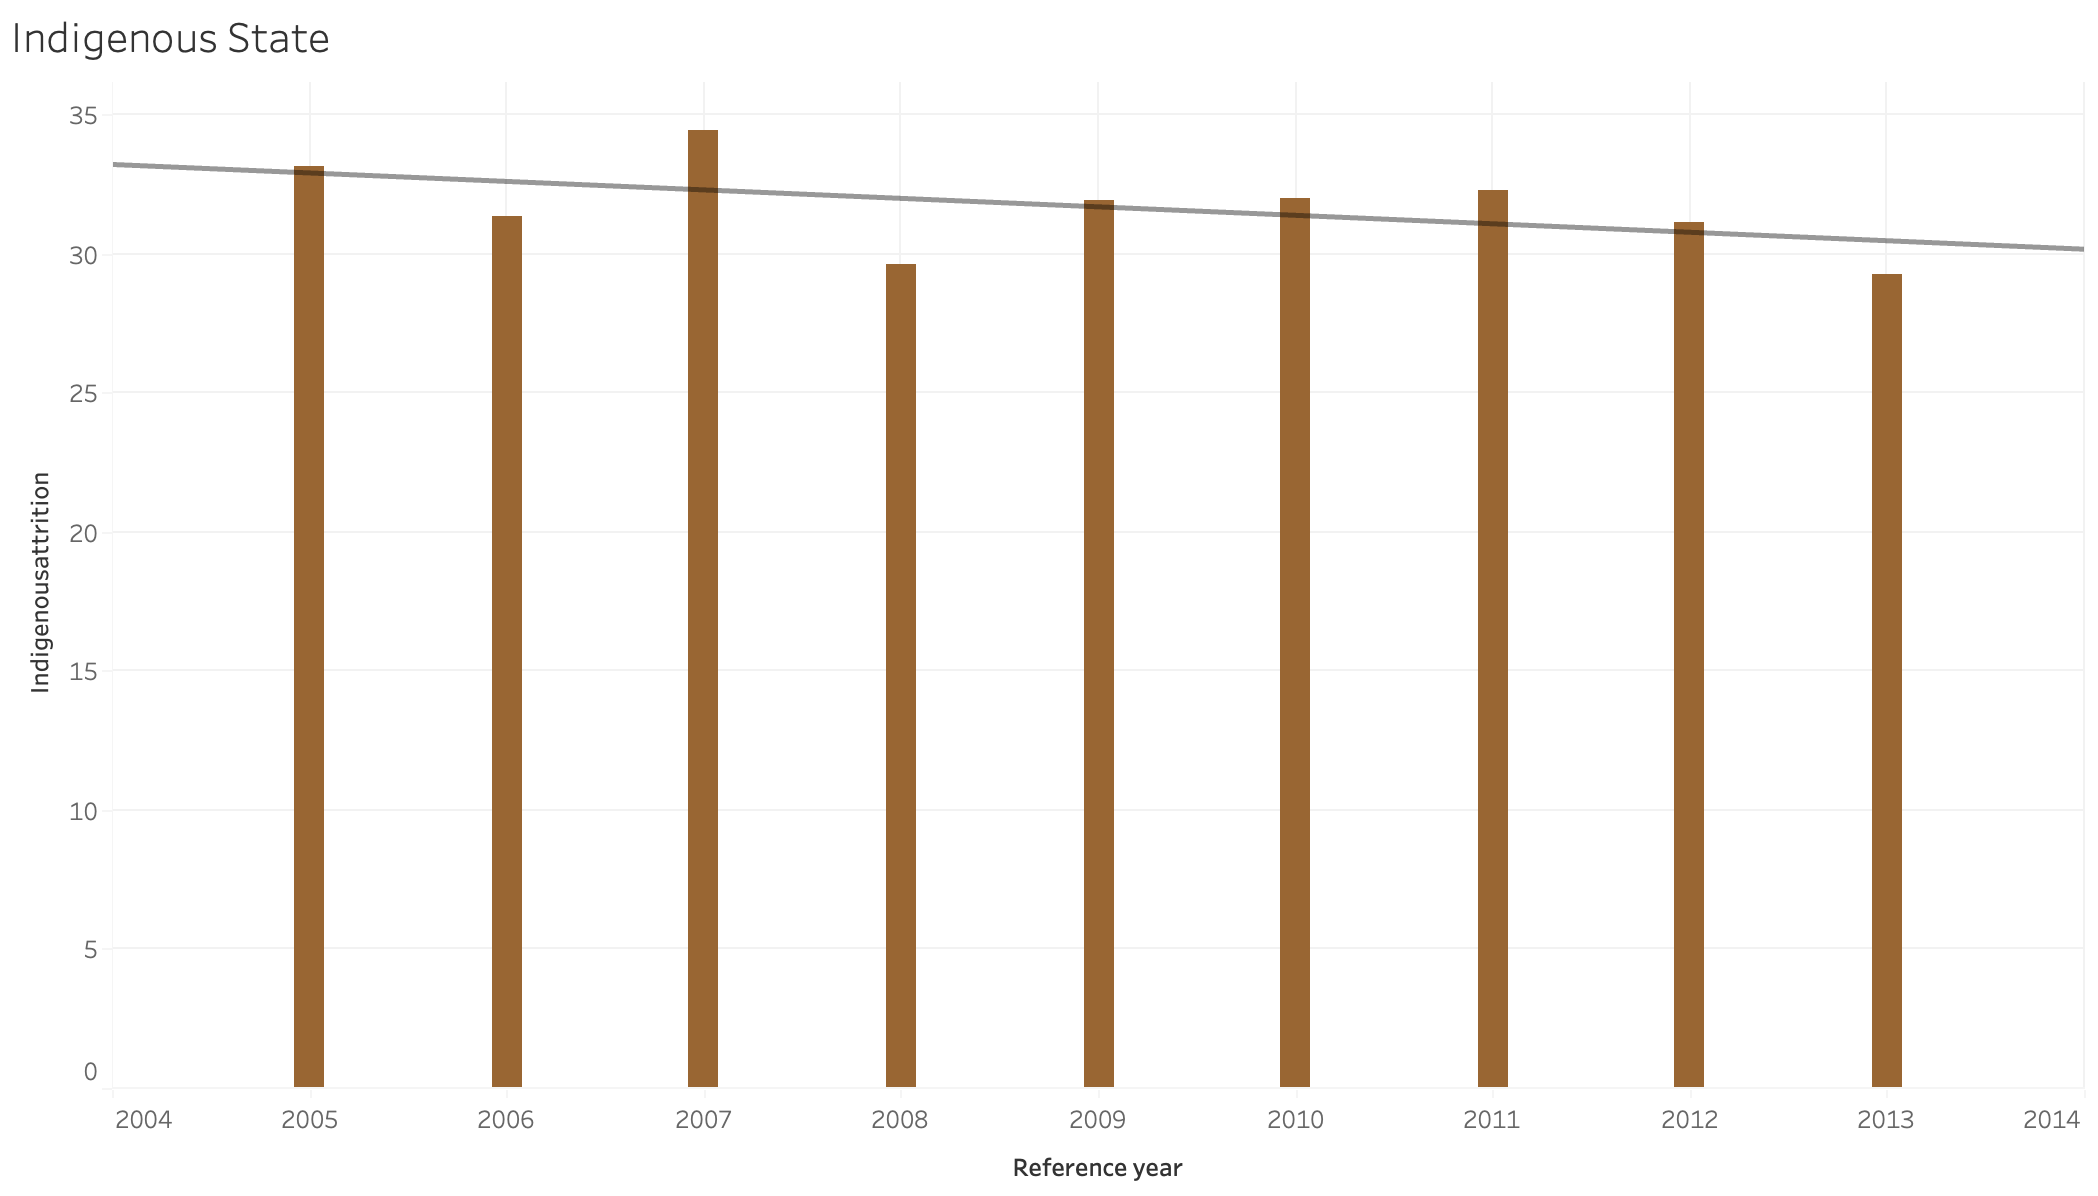
\includegraphics[width=0.4\textwidth]{images/Fig9.png} 
    \caption{Bar plot for attrition rate across years for Indigenous students} 
    \label{fig:bar5}
\end{figure}

\par From the plot, the following key observations are made: \begin{itemize} 
    \item Attrition rates for Indigenous students steadily decreased over the years, as seen in Figure \ref{fig:bar5}.
    \item The most significant drop occurred between 2009 and 2013. 
    \item 2013 recorded the lowest attrition rate, suggesting improvements in retention. 
    \item Increased access to scholarships, community support programs, and cultural inclusion initiatives likely contributed to this decline.
    \item Earthly brown color ,used in Figure \ref{fig:bar5}, chosen for representing attrition rates for Indigenous students due to its symbolic connection to land and cultural heritage. This color reflects respect for the traditional and cultural significance of Indigenous communities.
\end{itemize}

\textbf{Summary:} The gradual decrease in attrition rates for Indigenous students is likely due to enhanced educational support, government policies, and community-driven programs aimed at reducing barriers for Indigenous students.


\subsubsection{ATAR Score Analysis}

Figure \ref{fig:line3} shows attrition rates from 2005-2013 based on different ATAR scores, and Figure \ref{fig:pie3} shows the average attrition rate across these years for each ATAR range.

\begin{figure}[H] 
    \centering 
    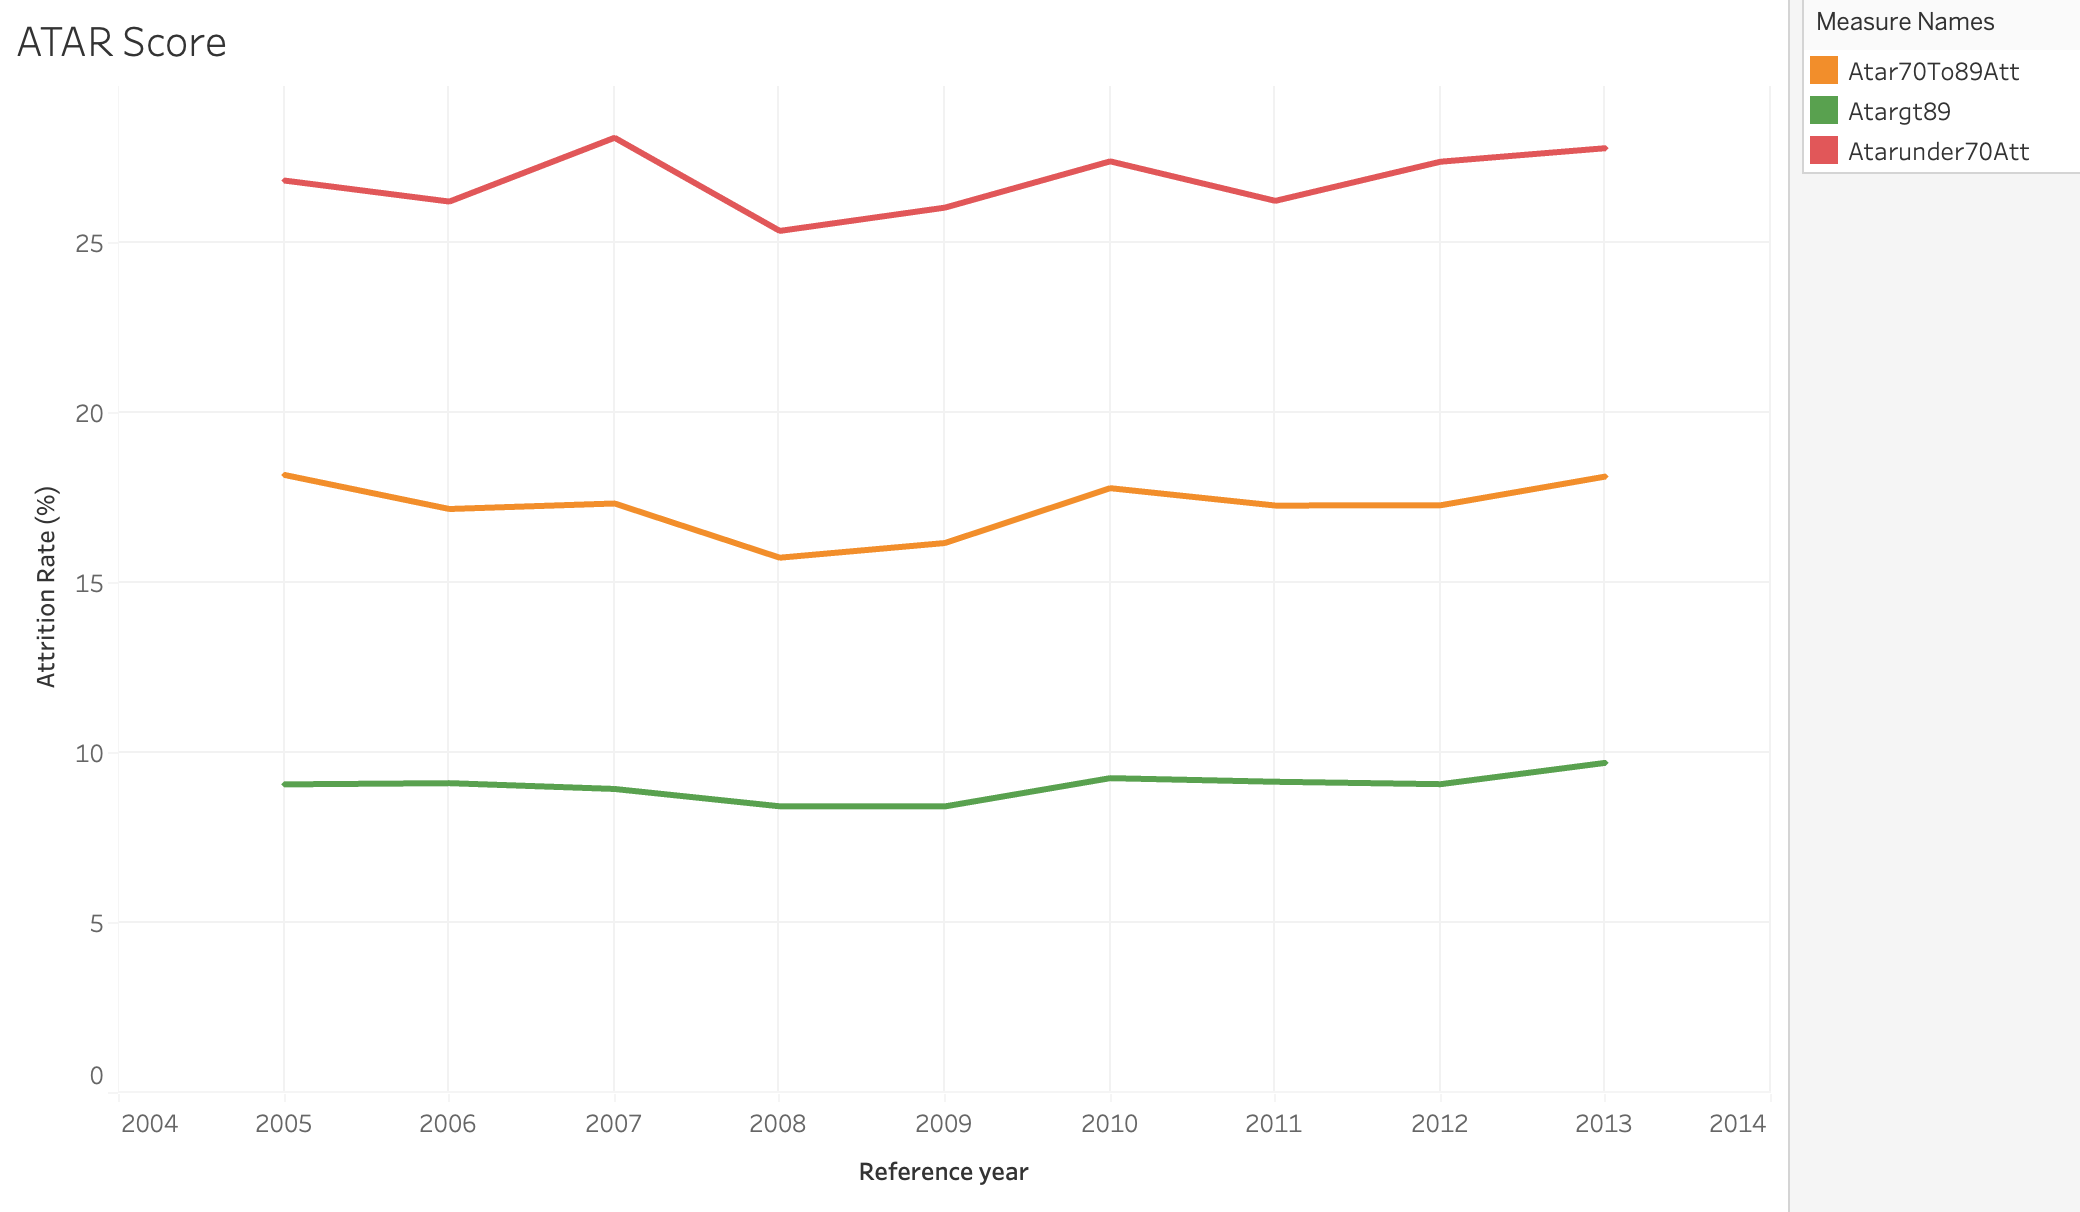
\includegraphics[width=0.4\textwidth]{images/Fig10.png} 
    \caption{Line chart for attrition rate across years based on different ATAR scores} 
    \label{fig:line3} 
\end{figure}

\begin{figure}[H] 
    \centering 
    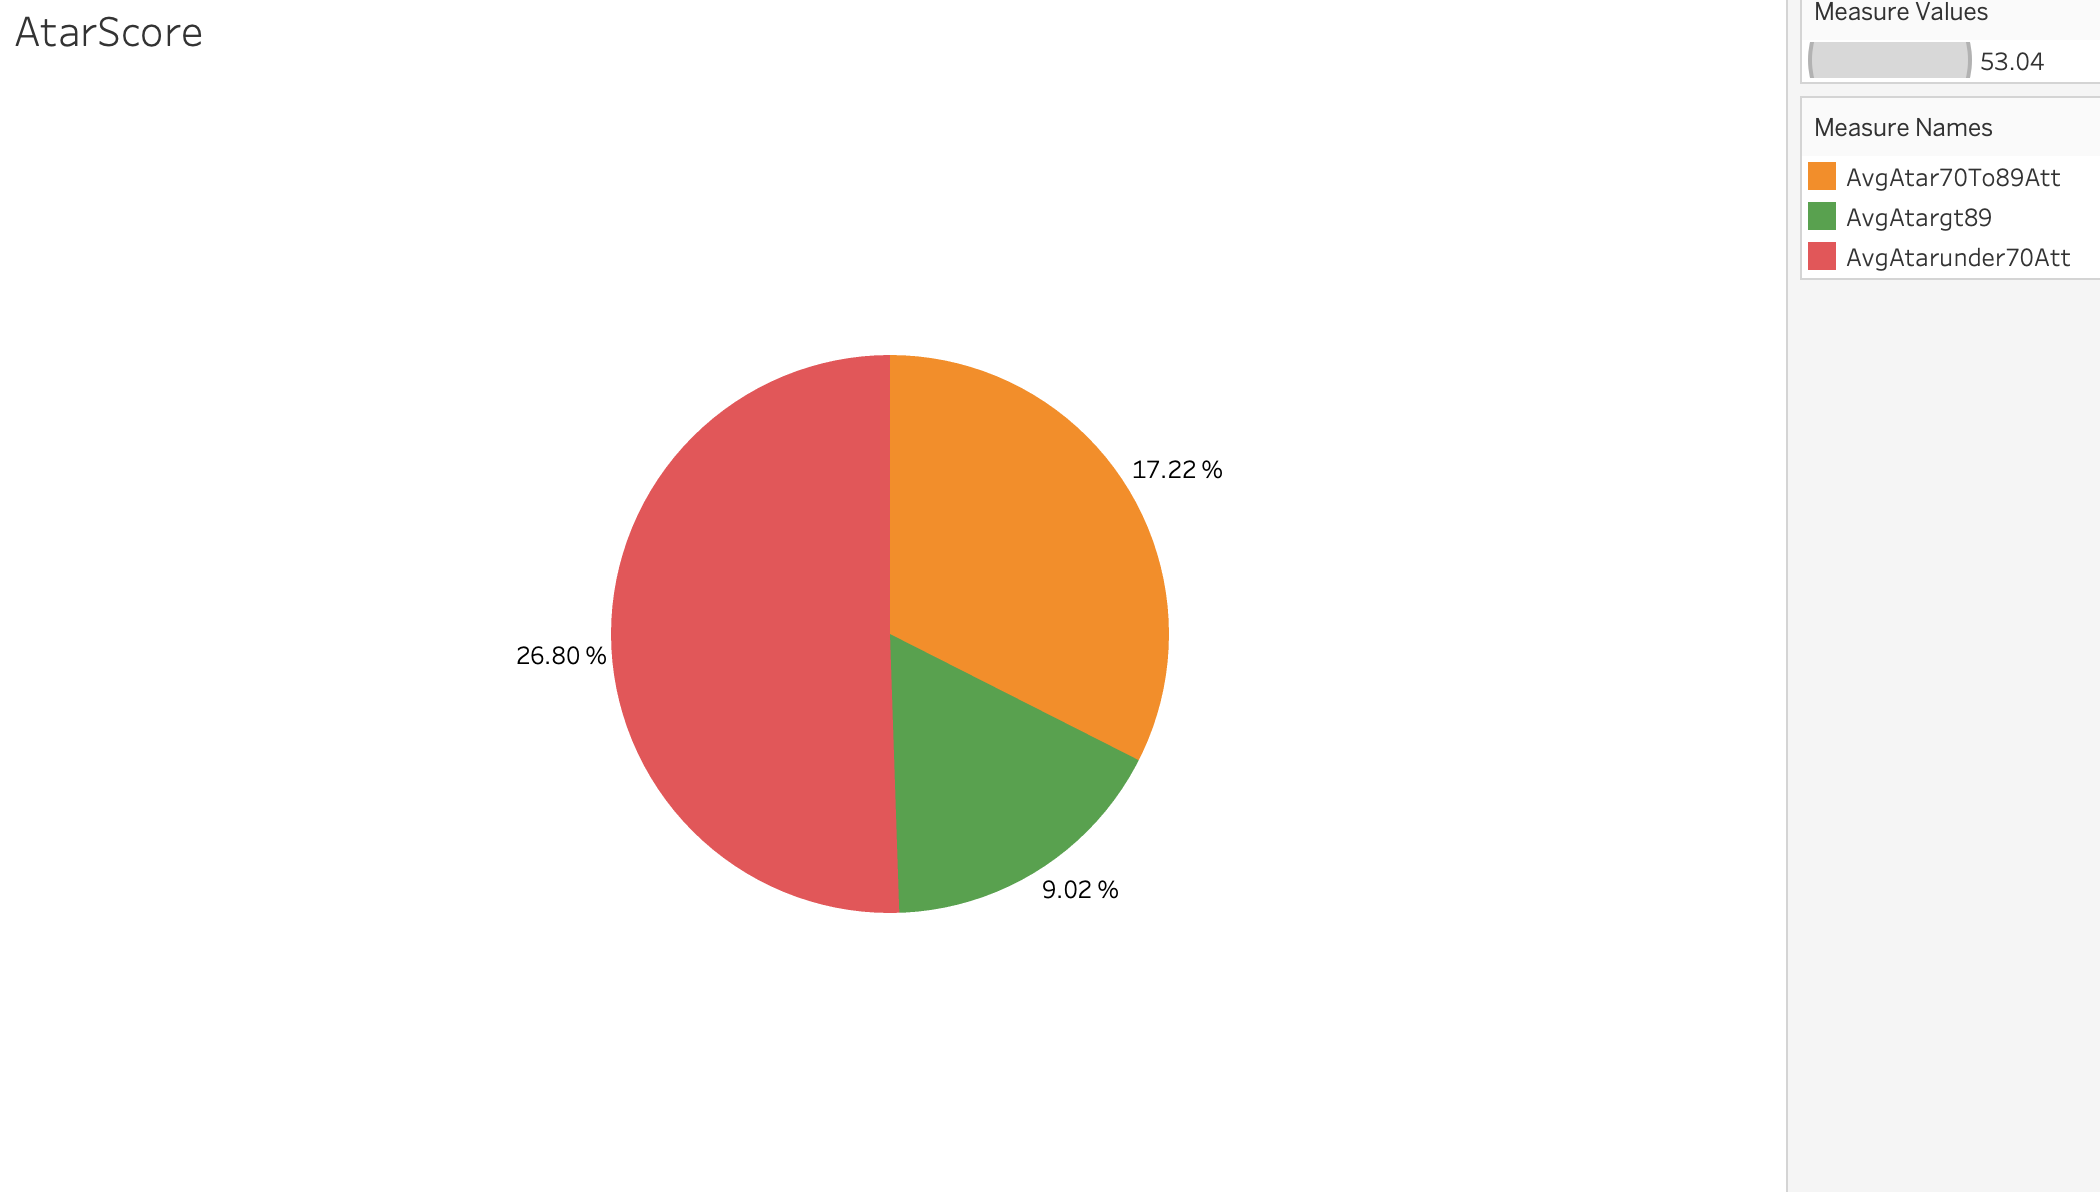
\includegraphics[width=0.4\textwidth]{images/Fig13.png} 
    \caption{Pie chart for average attrition rate across years based on different ATAR scores} 
    \label{fig:pie3}
\end{figure}

\par From the plot, the following key observations are made: 
\begin{itemize} 
    \item Figures \ref{fig:line3} and \ref{fig:pie3}
 show that students with ATAR scores of 90+ consistently have the lowest attrition rates, remaining constant over time.
    \item Students with ATAR scores below 70 exhibit the highest attrition rates, indicating academic challenges, as seen in the red section of Figure \ref{fig:pie3}. 
    \item The pie chart in Figure \ref{fig:pie3}, effectively visualizes the distribution of average attrition rates across different ATAR ranges using color differentiation. 
    \item The line chart in Figure \ref{fig:line3}, highlights the trend of attrition rates for various ATAR scores over the years.
    \item Colors are consistent across both charts: red for high attrition (urgent concern), orange for moderate attrition (caution), and green for low attrition (stability) rates.
\end{itemize}

\textbf{Summary:} Higher ATAR scores correlate with lower attrition rates, likely reflecting stronger academic preparedness, while students with lower ATAR scores struggle more, leading to higher dropout rates.

\subsubsection{Other Correlation Between Attributes}
Square graphs were plotted to analyze the relationship between gender and mode of study (Figure \ref{fig:square2}) and studying time and mode of study (Figure \ref{fig:square3}), because they effectively represent relationships between multiple categorical variables, allowing us to observe trends in attrition rates over time.

\begin{figure}[H] 
    \centering 
    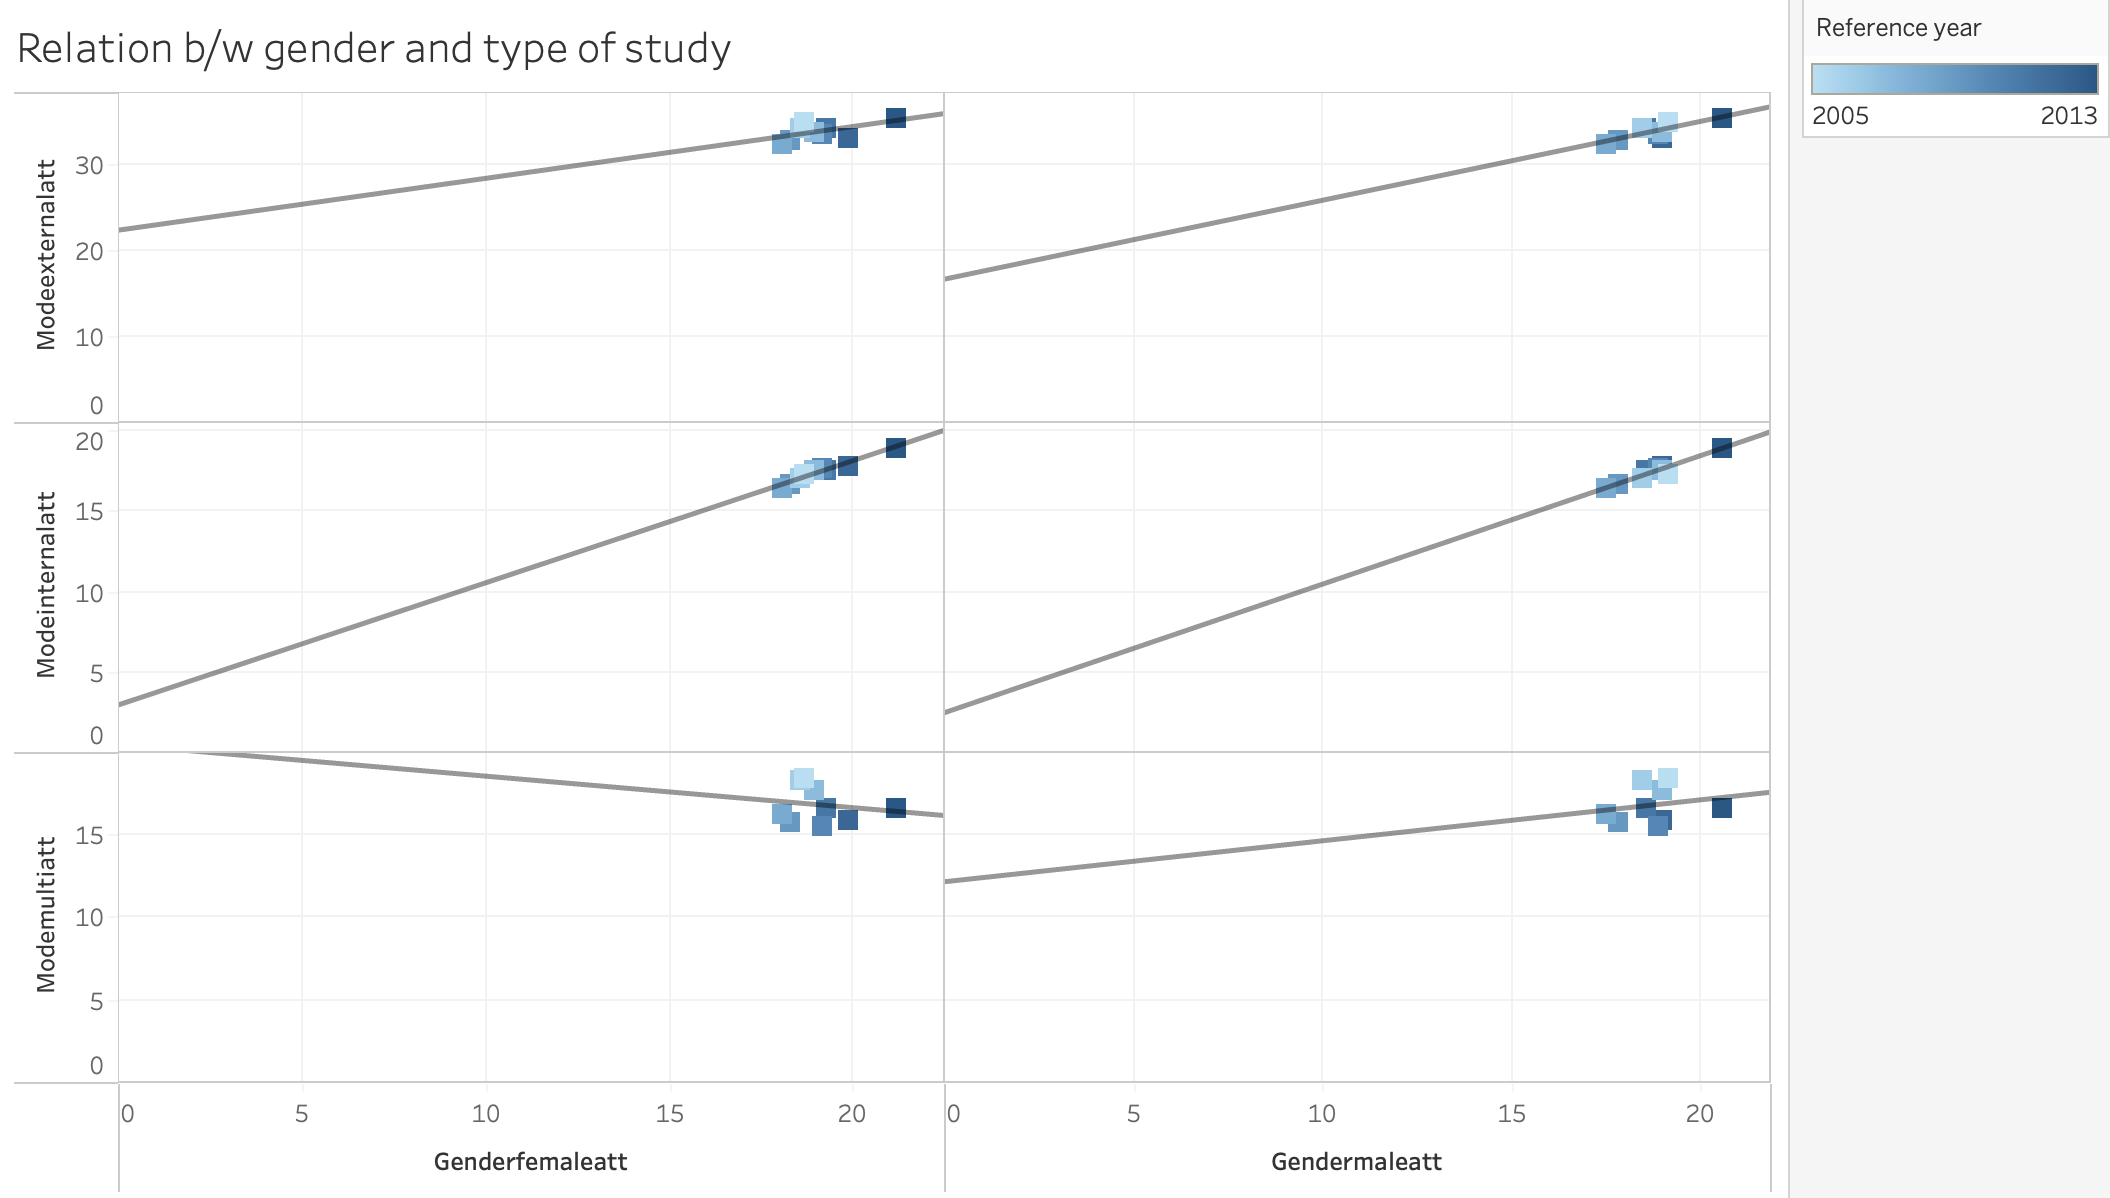
\includegraphics[width=0.4\textwidth]{images/Fig20.png} \caption{Square graph showing correlation between gender and mode of study for attrition rates.} 
    \label{fig:square2} 
\end{figure}

\begin{figure}[H] 
    \centering 
    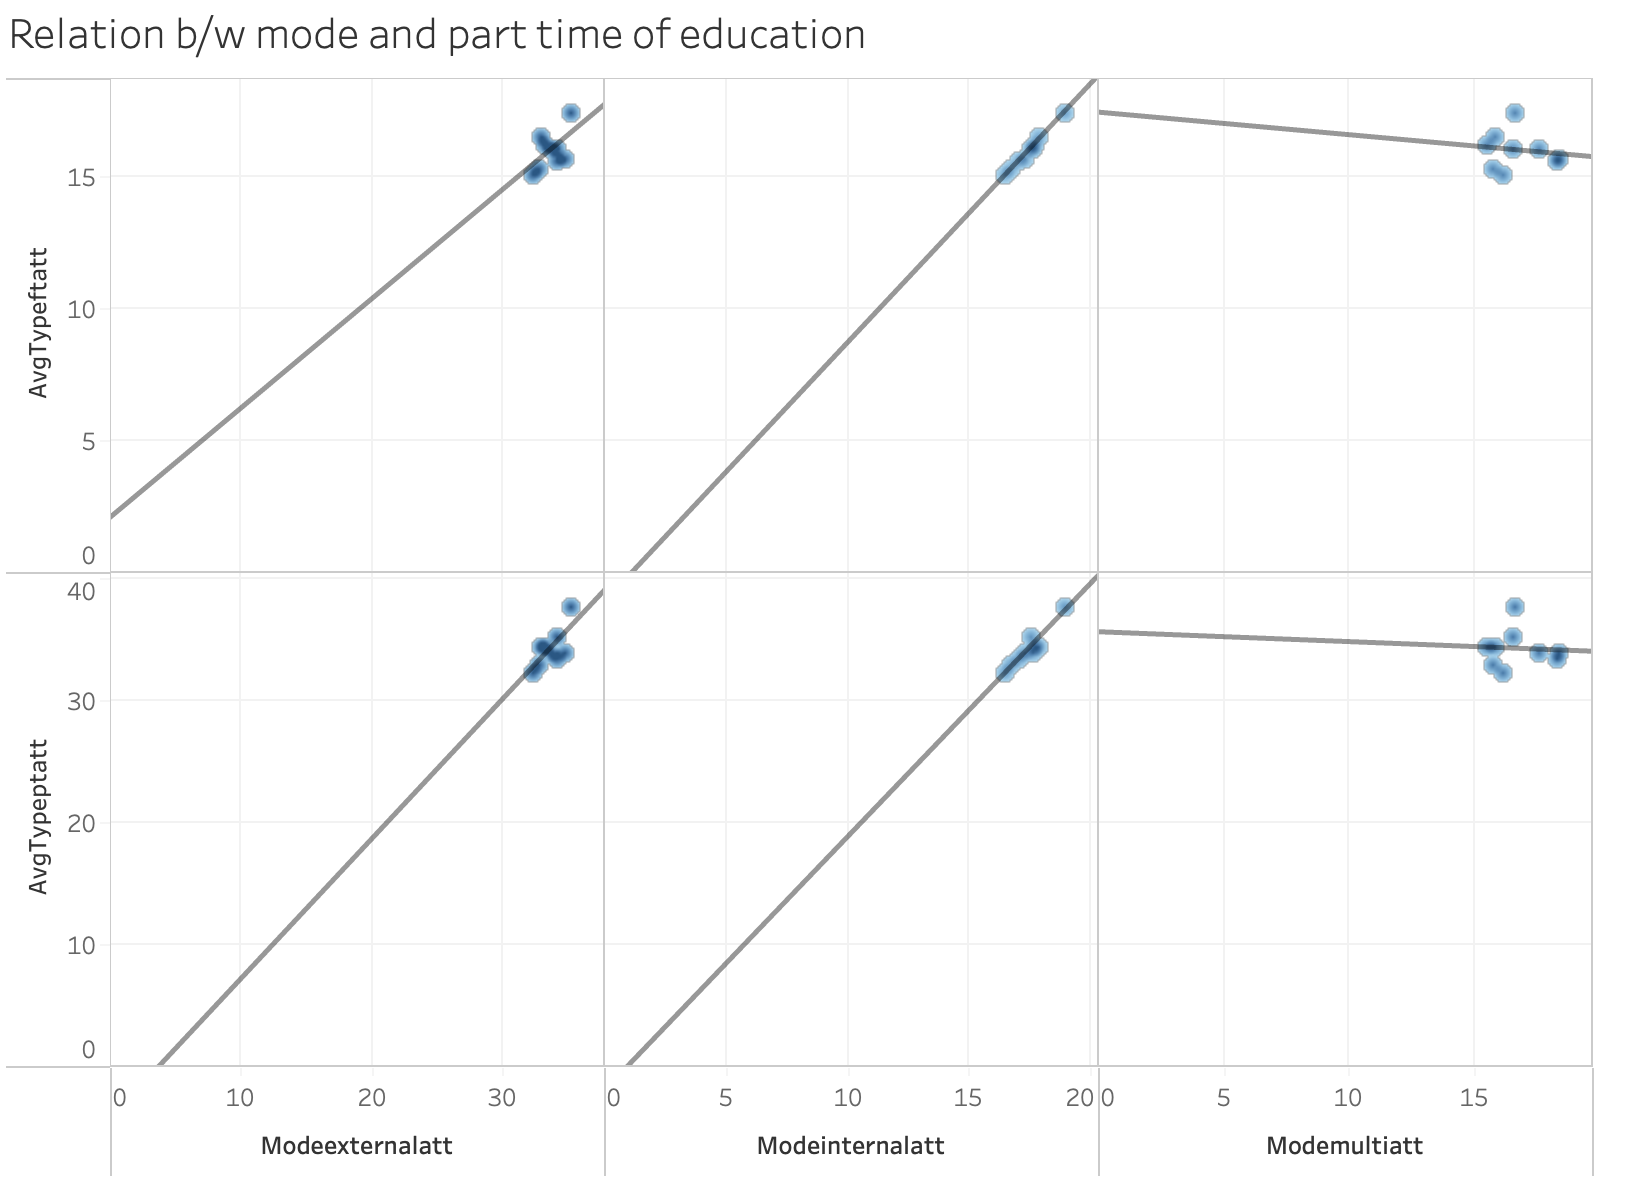
\includegraphics[width=0.4\textwidth]{images/Fig24.png} \caption{Square graph showing correlation between studying time and mode of study for attrition rates.} 
    \label{fig:square3} 
\end{figure}

\par From the plot, the following key observations are made: 
\begin{itemize} 
    \item Figure \ref{fig:square2} shows fewer female students in multi-mode programs are dropping out, likely due to improvements in blended learning, flexible schedules, and better resource access. 
    \item The same figure reveals higher dropout rates for male and female students in internal and external programs, with males in multi-mode programs also showing higher attrition. 
    \item Figure \ref{fig:square3} indicates lower dropout rates for both full-time and part-time students in multi-mode programs, suggesting greater flexibility and integration. 
    \item However, full-time and part-time students in internal and external programs display higher dropout rates, evidenced by the upward trend in the figure. 
    \item The square graph effectively visualizes these trends by clearly showing the relationship between the variables. \end{itemize}

\textbf{Summary:} Attrition rates for female students, as well as full-time and part-time students in multi-mode programs, show a declining trend. This is likely due to enhanced learning support systems, increased flexibility, and better resource access. The correlation suggests that multi-mode programs are becoming more inclusive and supportive, especially for diverse student groups.
\subsection{T2: Field of Study Analysis}
How do attrition rates vary across different fields of study?

\subsubsection{Student Admission Criteria Analysis}
Figures \ref{fig:stackbar1} and \ref{fig:treemap2} present the student admission criteria analysis. Figure \ref{fig:stackbar1} displays a stacked bar graph for attrition rates for different student admission criteria across several years, while Figure \ref{fig:treemap2} shows a horizontal bar chart of the average attrition rate for each criterion over the same period.

\begin{figure}[H]
    \centering
    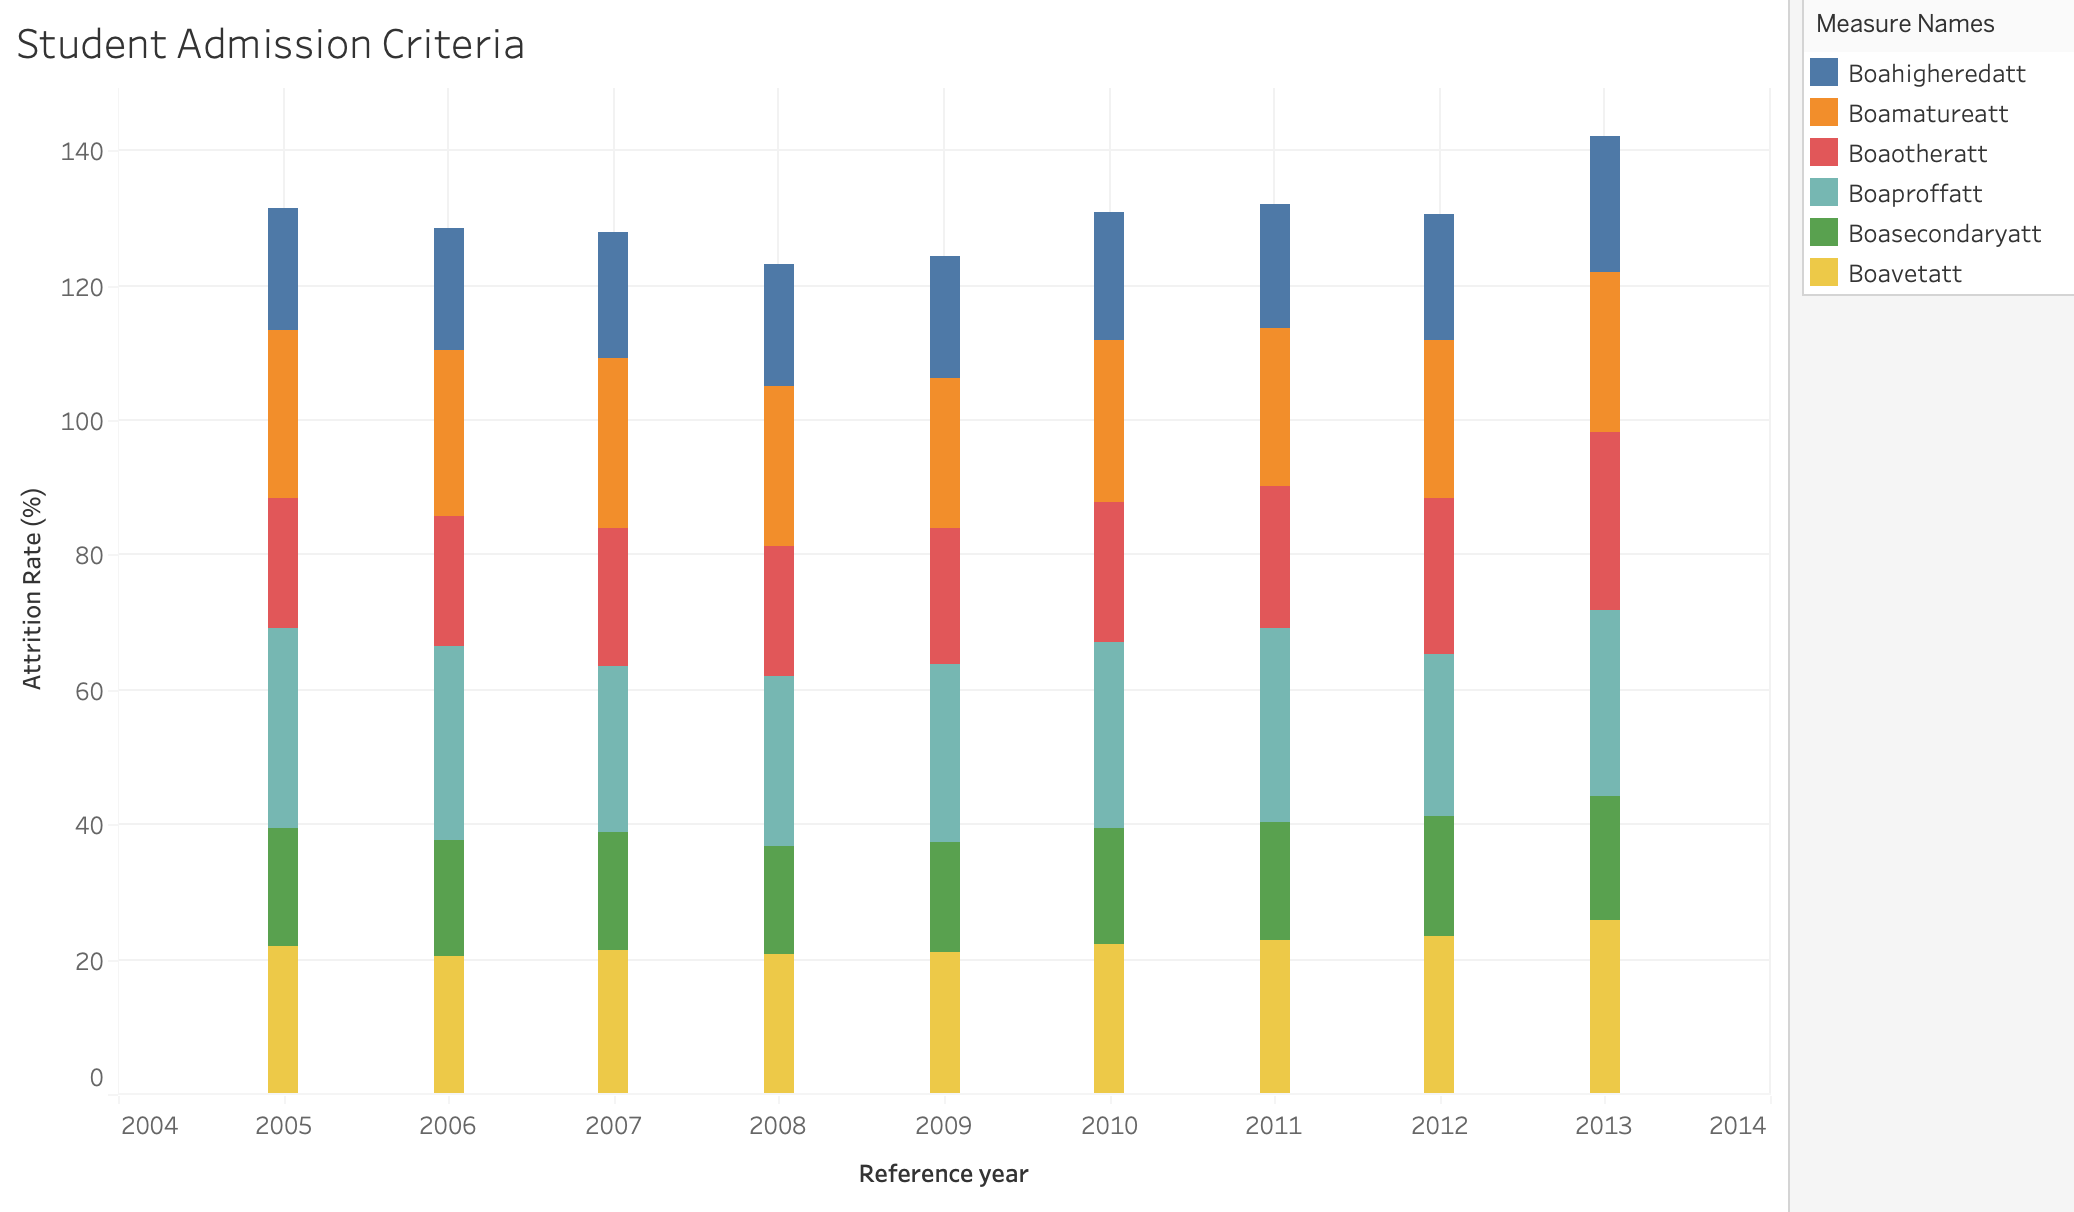
\includegraphics[width=0.4\textwidth]{images/Fig11.png}
    \caption{Stacked bar graph for attrition rates for different student admission criteria across different years}
    \label{fig:stackbar1}
\end{figure}

\begin{figure}[H]
    \centering
    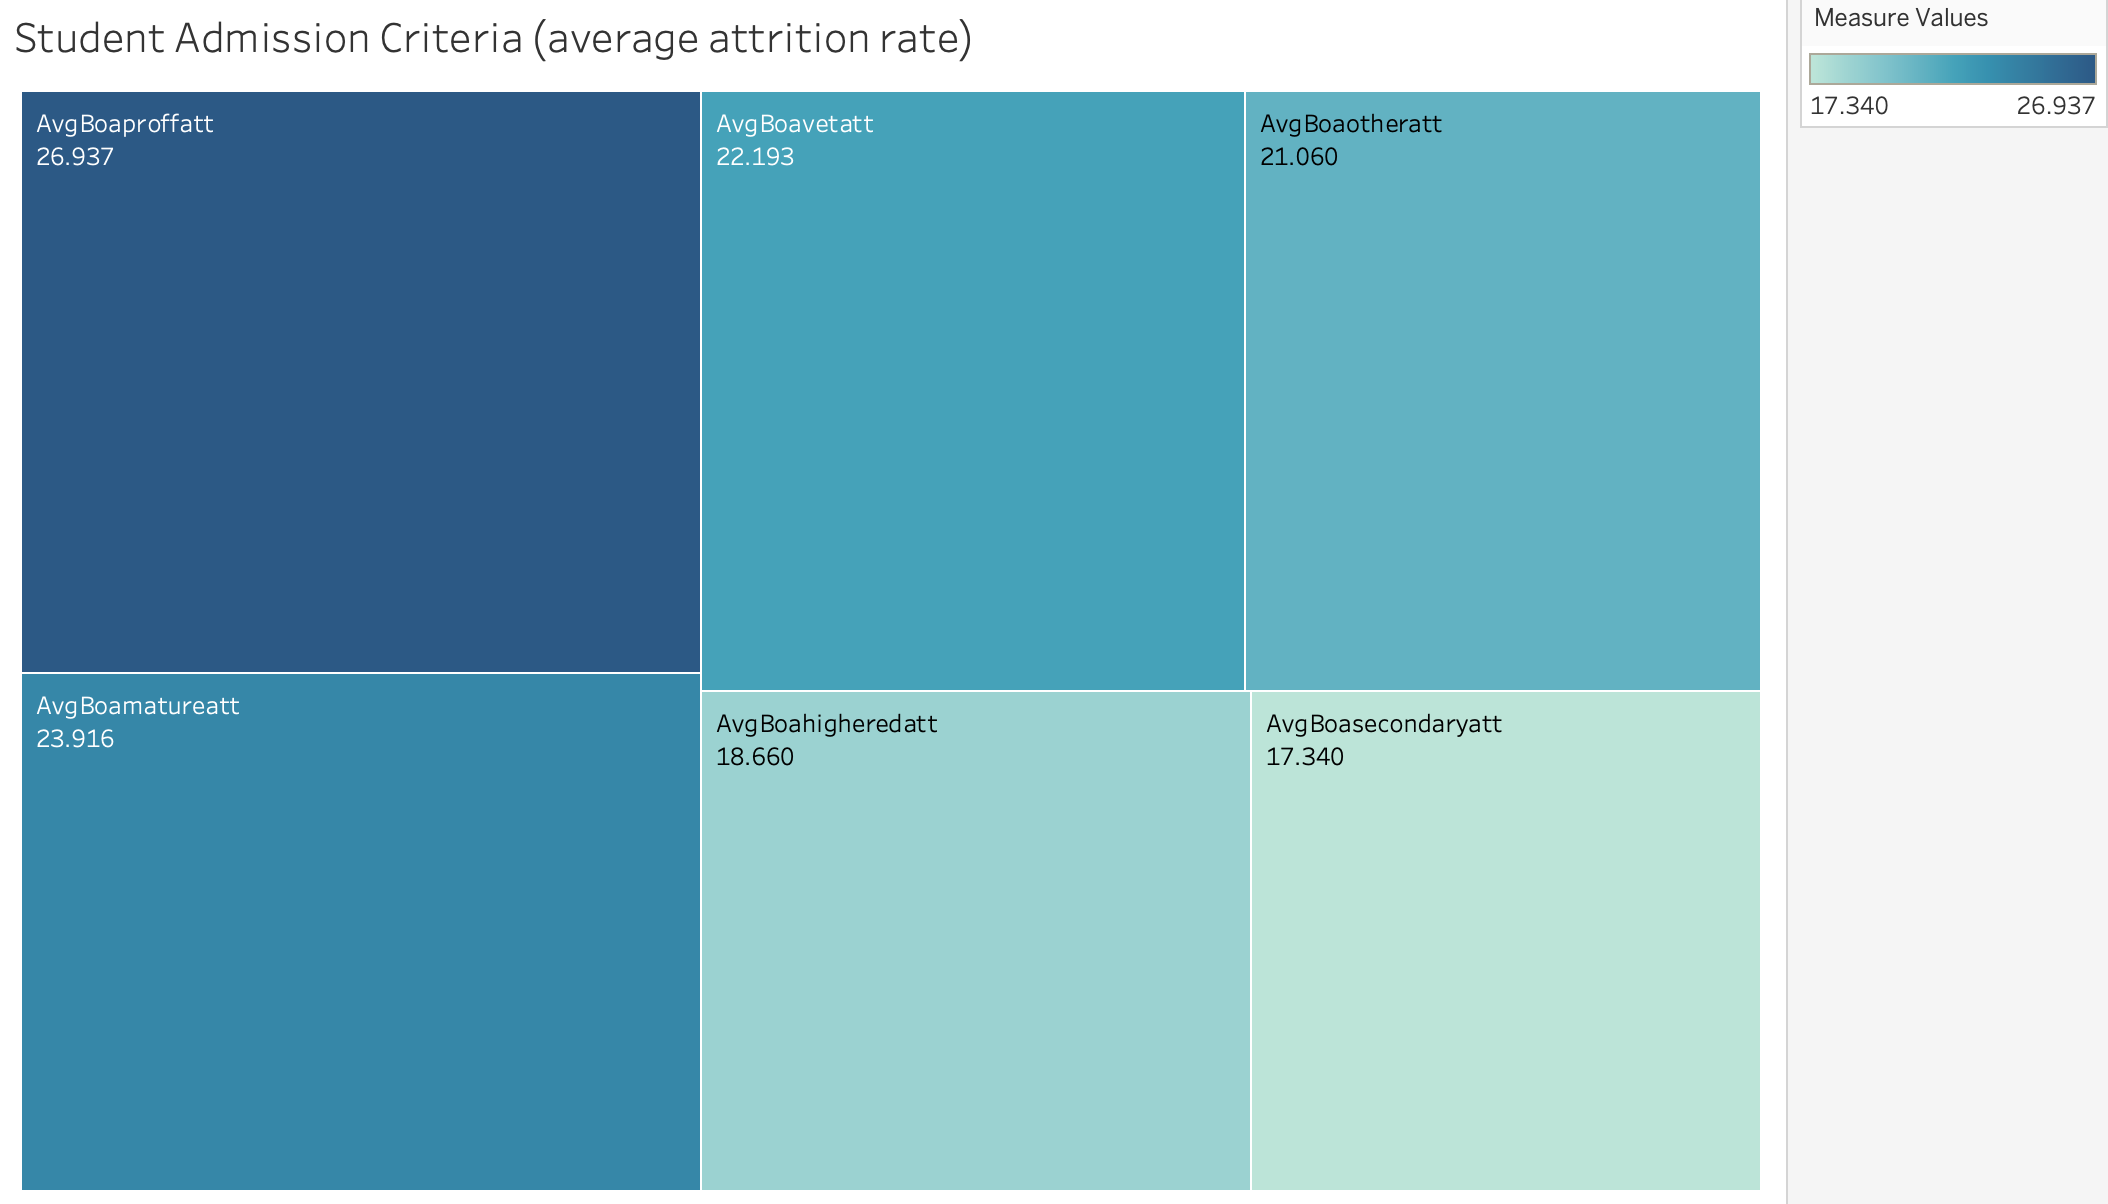
\includegraphics[width=0.4\textwidth]{images/Fig18.png}
    \caption{Tree Map showing the average attrition rate for different student admission criteria over the years.}
    \label{fig:treemap2}
\end{figure}

From these plots, the following key observations are made:
\begin{itemize} 
    \item Figure \ref{fig:stackbar1} shows similar overall attrition trends across different years, with the lowest rate in 2008.
    \item Figure \ref{fig:stackbar1} illustrates how each student admission pathway contributes to the overall attrition, using distinct colors for clarity.
    \item Figure \ref{fig:treemap2} confirms that Boaproffatt has the highest average attrition rate, while Boasecondaryatt (admission via secondary education) contributes the least.
    \item The stacked bar chart in Figure \ref{fig:stackbar1} demonstrates the impact of each student admission criteria on attrition rate across years, using distinct colors.
    \item The tree map in Figure \ref{fig:treemap2} ranks average attrition rates for student admission criteria
from highest to lowest.
    \item Colors are consistent across both charts, ensuring clarity and ease of comparison.
\end{itemize}

The color scheme used across both figures is designed to provide clear and consistent information. In Figure \ref{fig:stackbar1}, Boaproffatt is shown in light blue to highlight its consistently high attrition rate, indicating significant challenges for students with professional qualifications. Boamatureatt is represented in orange, reflecting its moderately high attrition rate, which may be due to the difficulties mature students face in balancing work and study. Boavetatt is depicted in yellow, showing a stable but noticeable attrition rate, suggesting that students from vocational backgrounds might need extra support. Boaotheratt is shown in red to emphasize its variable attrition rates, which could be due to the unpredictability of non-standard admission pathways. In Figure \ref{fig:treemap2}, these color choices are maintained to allow easy comparison and interpretation of the average attrition rates.

\textbf{Summary:} The analysis of attrition rates based on student admission criteria reveals that students admitted via professional qualifications (Boaproffatt) consistently exhibit the highest attrition rates, suggesting a need for tailored support. In contrast, those admitted through secondary education (Boasecondaryatt) have the lowest rates, indicating stronger academic preparation. Mature age (Boamatureatt) and VET course entrants (Boavetatt) also show moderate attrition, reflecting potential challenges specific to these groups. Boaotheratt’s variable rates across years emphasize the need for personalized academic support. These insights highlight the importance of targeted interventions to reduce attrition across diverse admission pathways.



\subsubsection{Background Education of Student Analysis}
Figures \ref{fig:stackbar2} and \ref{fig:treemap1} present the background education of student analysis. Figure \ref{fig:stackbar2} displays a stacked bar graph for attrition rate for different education backgrounds across several years, while Figure \ref{fig:treemap1} shows a tree map of the average attrition rate for different education backgrounds over the same period.

\begin{figure}[H]
    \centering
    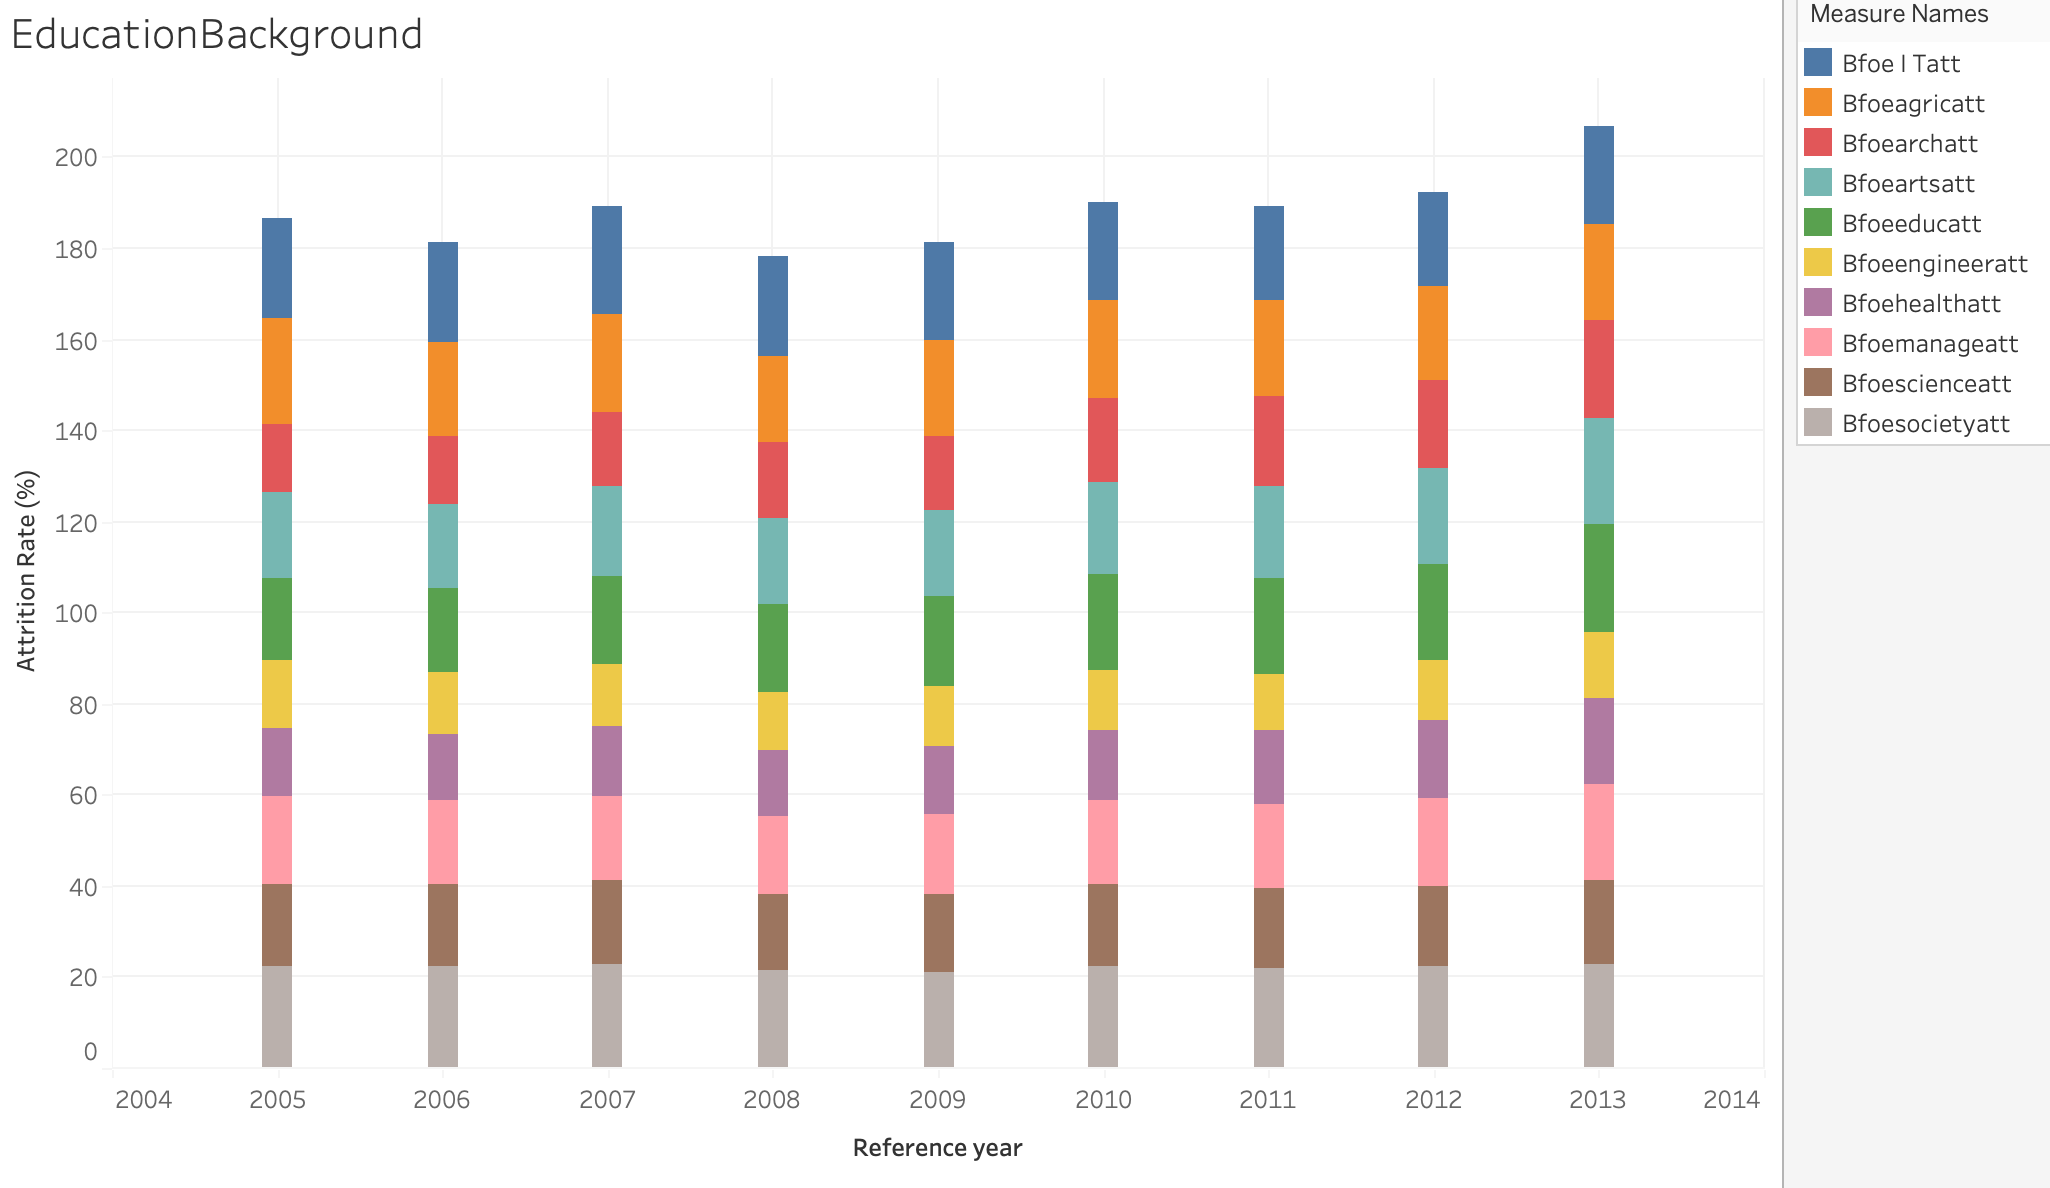
\includegraphics[width=0.4\textwidth]{images/Fig12.png}
    \caption{Stacked bar graph for attrition rate for different education backgrounds across different years}
    \label{fig:stackbar2}
\end{figure}

\begin{figure}[H]
    \centering
    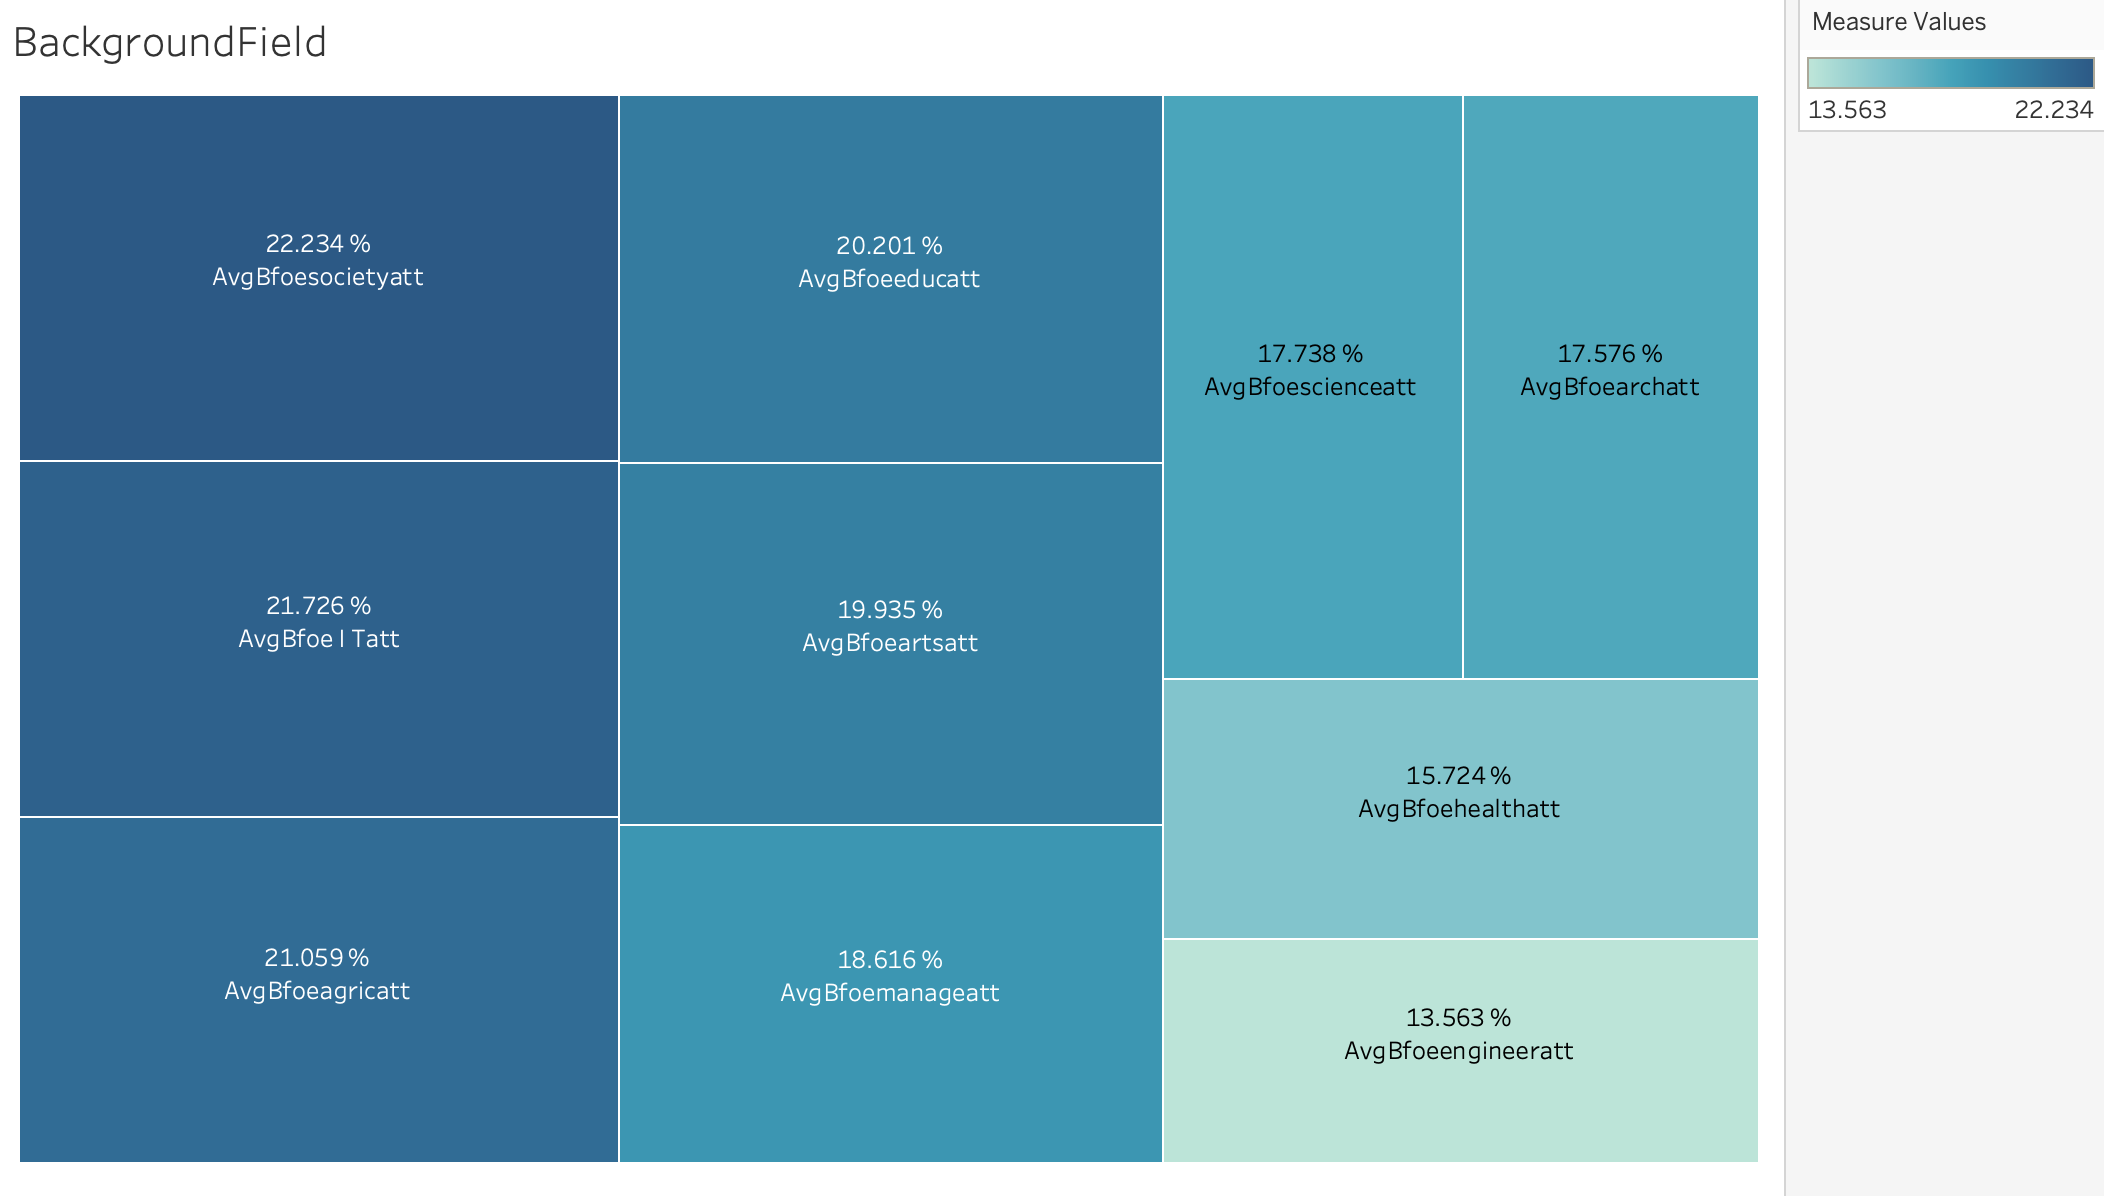
\includegraphics[width=0.4\textwidth]{images/Fig17.png}
    \caption{Tree Map showing the average attrition rate for different education backgrounds over the years.}
    \label{fig:treemap1}
\end{figure}

From these plots, the following key observations are made:
\begin{itemize} 
    \item Figure \ref{fig:stackbar2} shows similar overall attrition trends across different years, with the lowest rate in 2008.
    \item Figure \ref{fig:stackbar2} highlights higher attrition rates for Bfoesocietyatt (grey), Bfoe | Tatt (dark blue), and Bfoeagriatt (orange).
    \item Figure \ref{fig:treemap1} confirms these findings, showing consistent color for higher attrition rates at left side, while Bfoeengineeringatt (yellow) has the lowest rate(at bottom right in Figure \ref{fig:treemap1}).
    \item The stacked bar chart in Figure \ref{fig:stackbar2} demonstrates the impact of each field of education on overall attrition, using distinct colors.
    \item The tree map in Figure \ref{fig:treemap1} ranks average attrition rates from highest to lowest.
    \item Colors are consistent across both charts, ensuring clarity and ease of comparison.
\end{itemize}

\par Agriculture and Creative Arts show the highest attrition rates due to limited career opportunities and financial instability. Conversely, Engineering and Health have the lowest attrition rates, reflecting strong job prospects. Natural and Physical Sciences, Information Technology, and Education exhibit moderate attrition rates influenced by steady demand and varying job market conditions. Management and Commerce also show moderate rates due to a dynamic job market. Society and Culture, and Architecture have higher attrition rates due to less direct career pathways and industry competitiveness.

\textbf{Summary:} The analysis indicates that fields with high attrition rates, such as Agriculture and Creative Arts, are often linked to limited career opportunities and financial instability. Conversely, fields like Engineering and Health, with low attrition rates, benefit from strong job prospects and high demand. Other fields exhibit moderate attrition rates, reflecting a balance between market demand and career stability.
% \subsubsection{Other correlations between attributes:}
% A scatter plot (Figure \ref{fig:scatter1}) is plotted for different attributes which shows abnormalities for attrition across years.
% \begin{figure}[H]
%     \centering
%     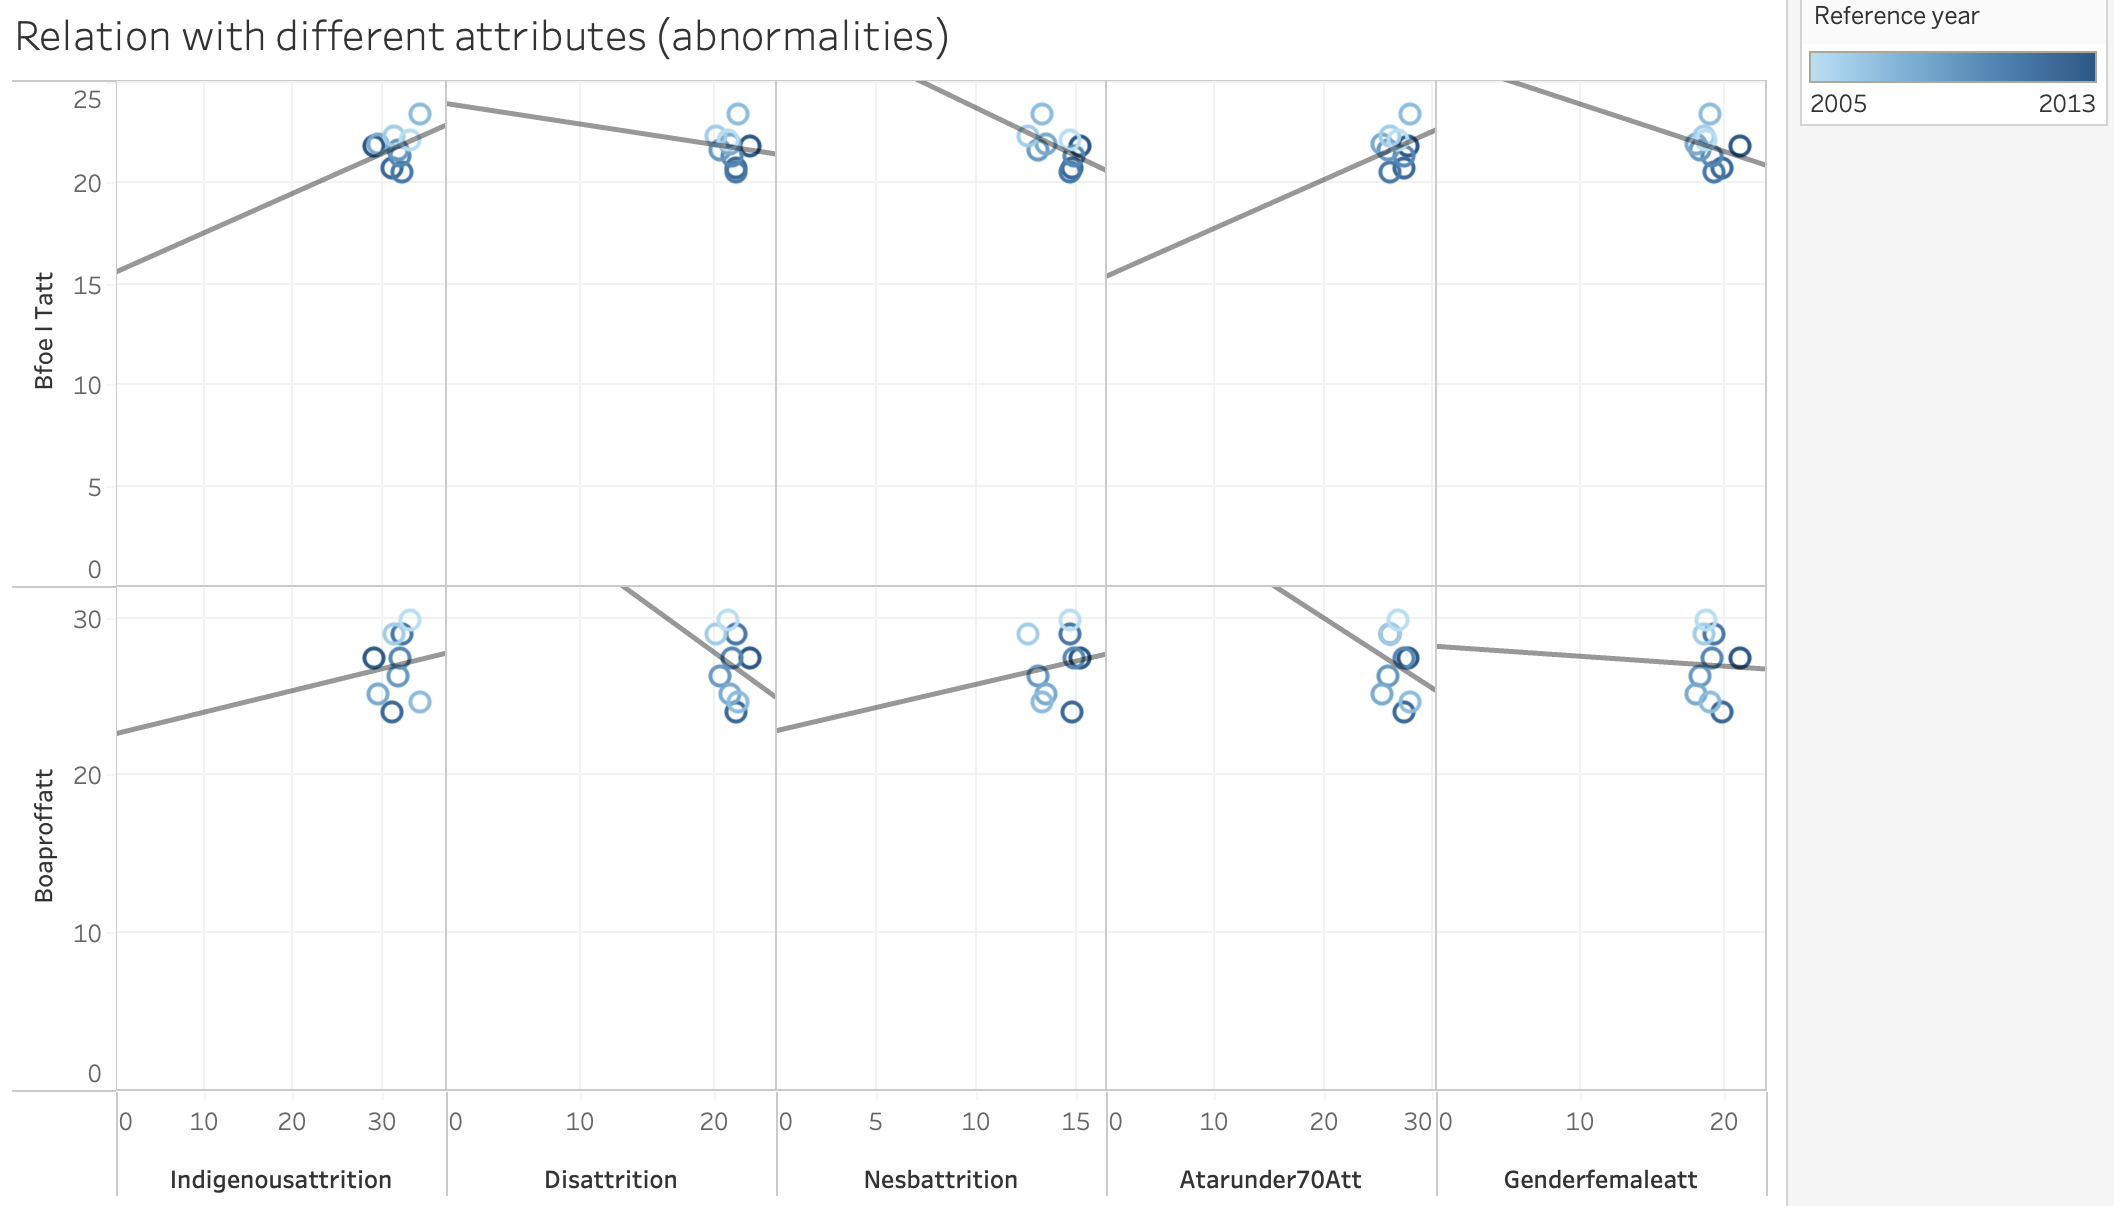
\includegraphics[width=0.4\textwidth]{images/Fig33.png}
%     \caption{Scatter plot showing different attributes which shows abnormalities for attrition across years.}
%     \label{fig:scatter1}
% \end{figure}
% Keys observations and insights from the plot are:
% \begin{itemize} 
%     \item IT Field: Figure \ref{fig:scatter1} indicates a declining attrition trend for disabled, non-English-speaking, and female students in IT, likely due to improved support systems. 
%     \item Professional Qualification Admissions: Students admitted based on professional qualifications show reduced attrition rates, particularly for females, disabled students, and those with ATAR scores below 70, potentially due to targeted assistance programs.
%     \item Trend line are used to analyze various attributes over time period with other attributes.
% \end{itemize}

\subsection{T3: Geographical Analysis}
 Are there any regional differences in attrition rates across Australia?
\indent \textbf{Note:} Some SA3 / LGA regions were missing in the dataset. To avoid null values, we assigned the minimum attrition rate observed across all years. As a result, the left part of the map consistently shows a lighter shade of teal blue, indicating the missing SA3 / LGA regions.
\subsubsection{Based on SA3 area analysis:}
Figure \ref{fig:mainfigure1} and \ref{fig:mainfigure2} shows different heat map for attrition rate across different years from 2005-2013 according to SA3 regions of Australia.

\begin{figure}[H]
    % First row of subfigures
    \centering
    \vskip15pt
    \subfloat[Heat map for 2005]{ % Manually manage the numbering
        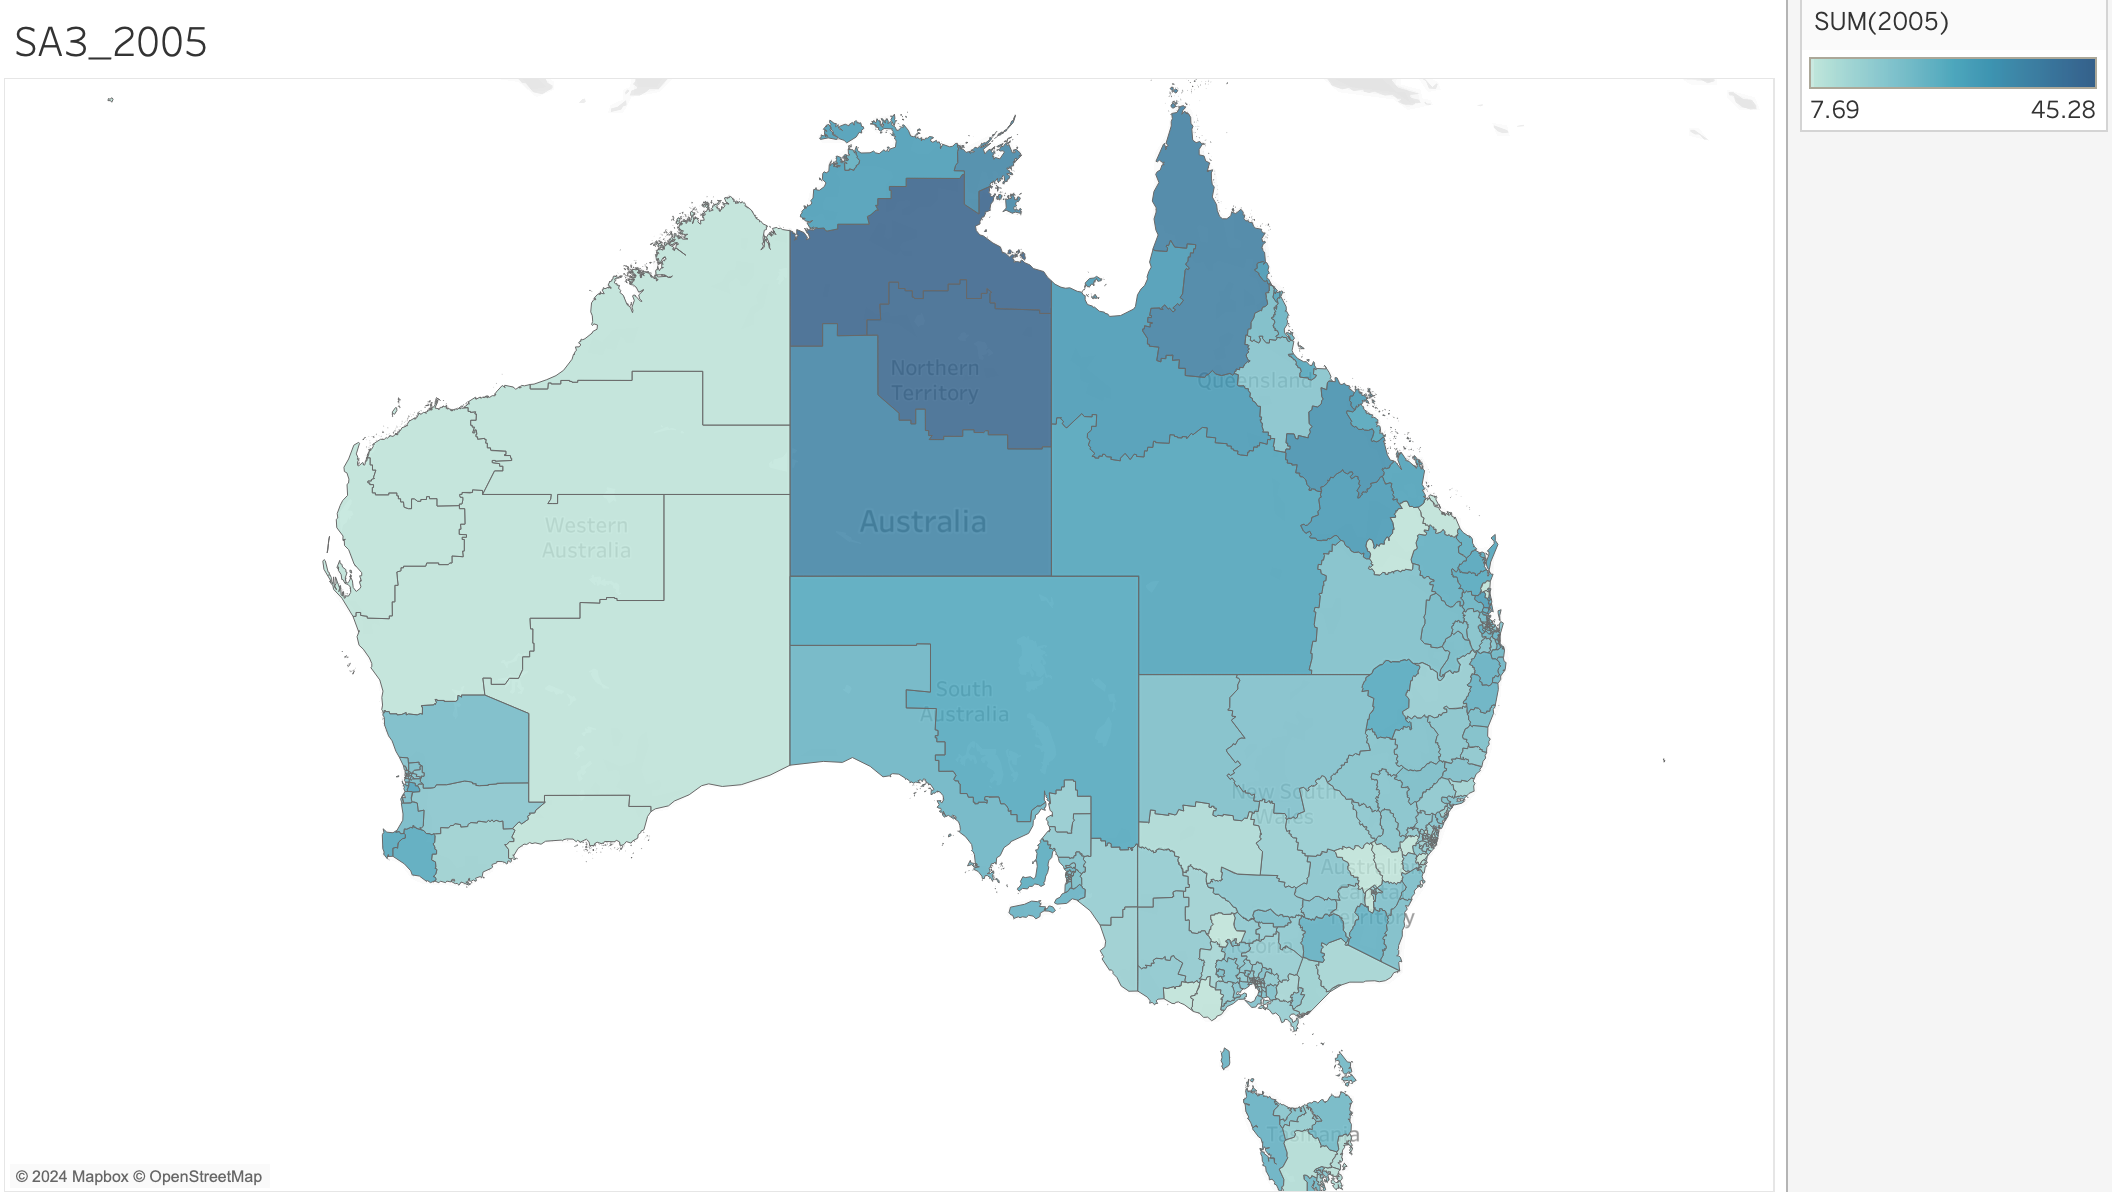
\includegraphics[width=0.45\textwidth]{images/Fig27.1.png}
        \label{fig:subfig1}
    }
    \caption{Heat maps for SA3 areas 2005 to 2013 (Part 1).}
    \label{fig:mainfigure1}
\end{figure}
\clearpage

\begin{figure*}[t]
    % Second row of subfigures
    \centering
    \subfloat[Heat map for 2006]{ % Continue numbering from the previous figure
        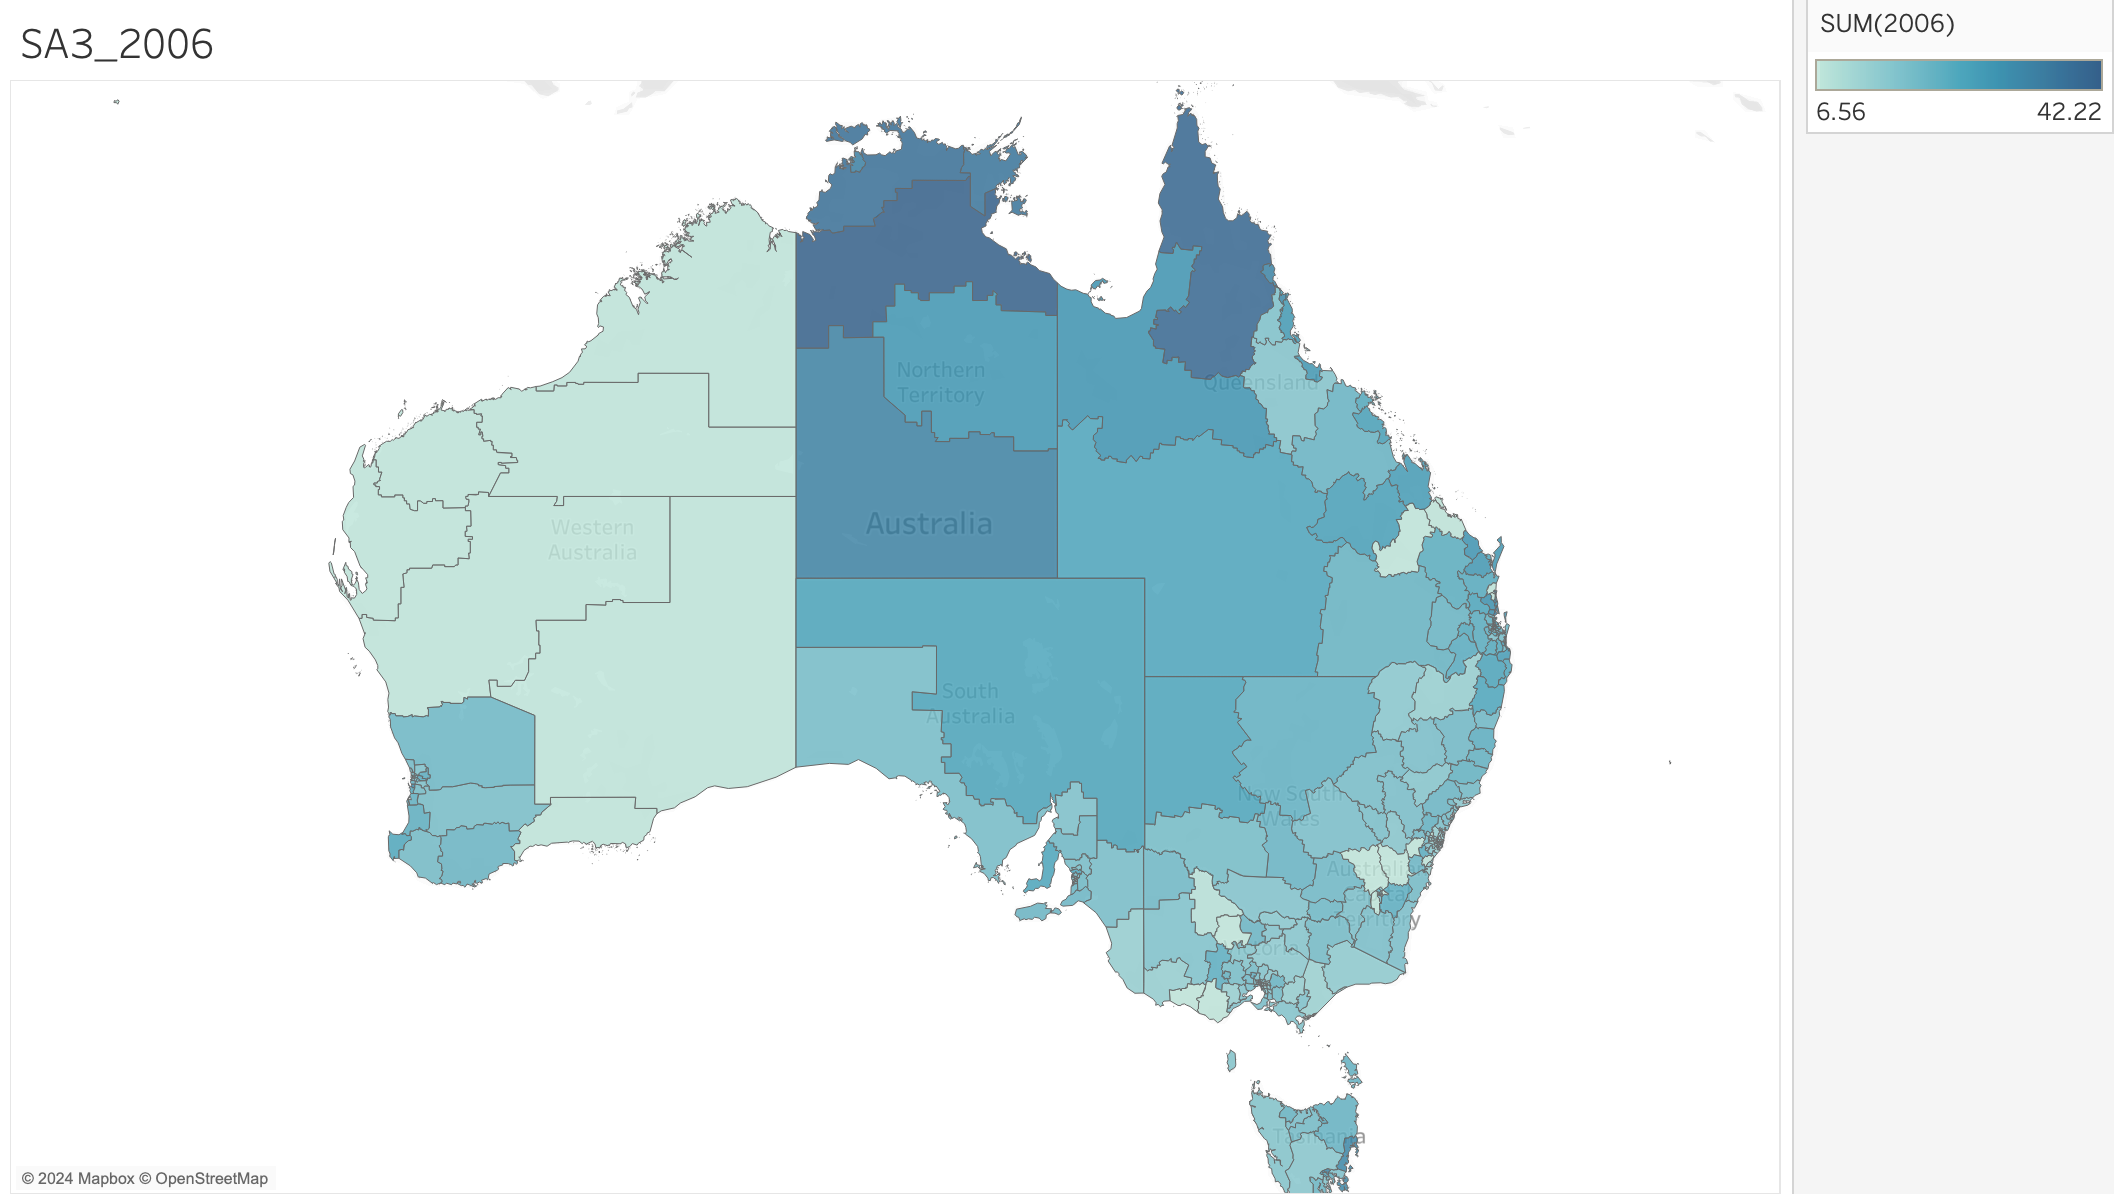
\includegraphics[width=0.45\textwidth]{images/Fig27.2.png}
        \label{fig:subfig2}
    }
    \hfill
    \subfloat[Heat map for 2007]{ 
        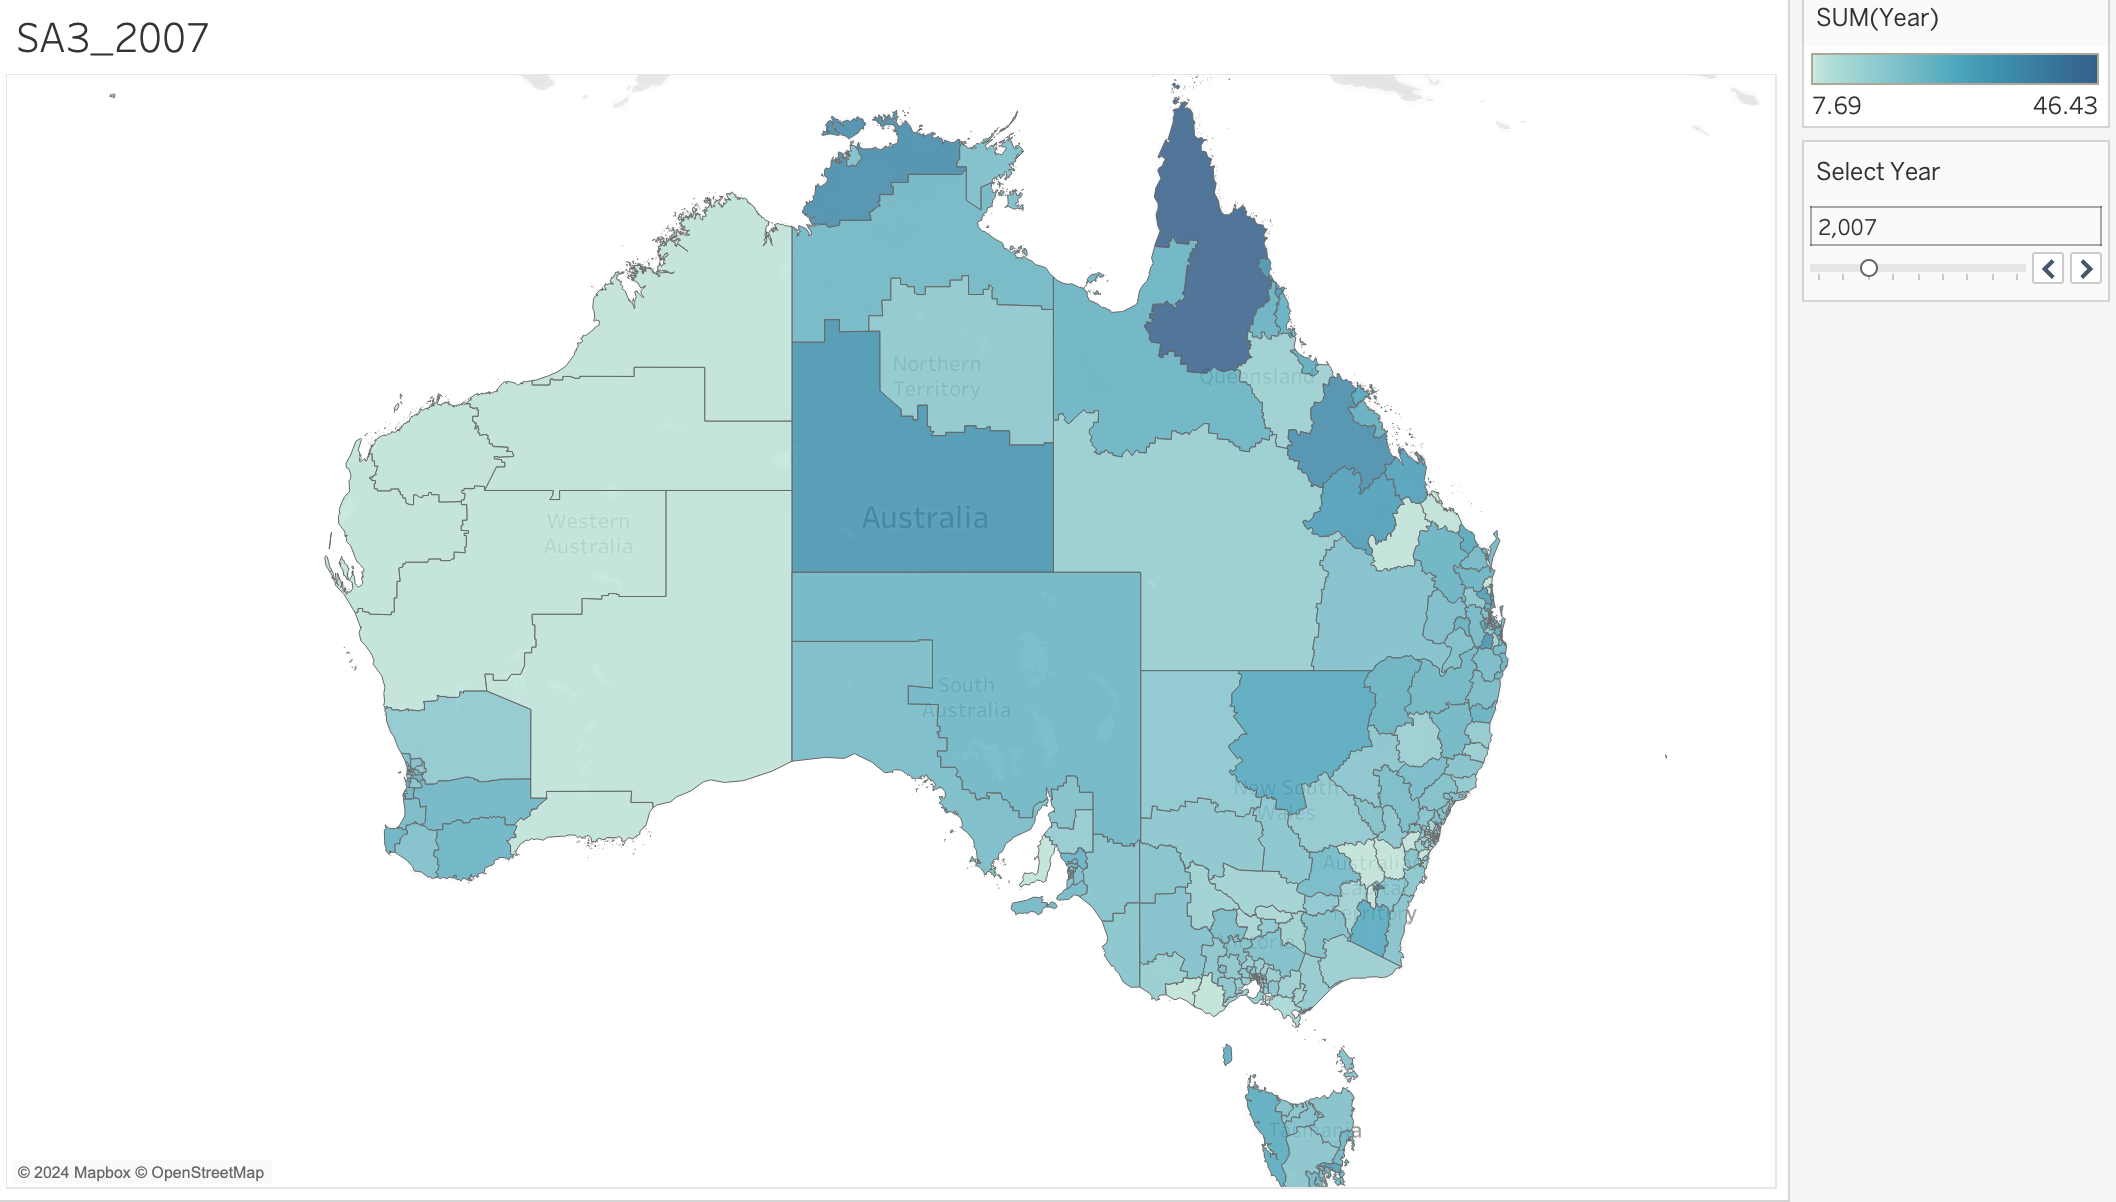
\includegraphics[width=0.45\textwidth]{images/Fig27.3.png}
        \label{fig:subfig3}
    }
    \vskip10pt
    \subfloat[Heat map for 2008]{ 
        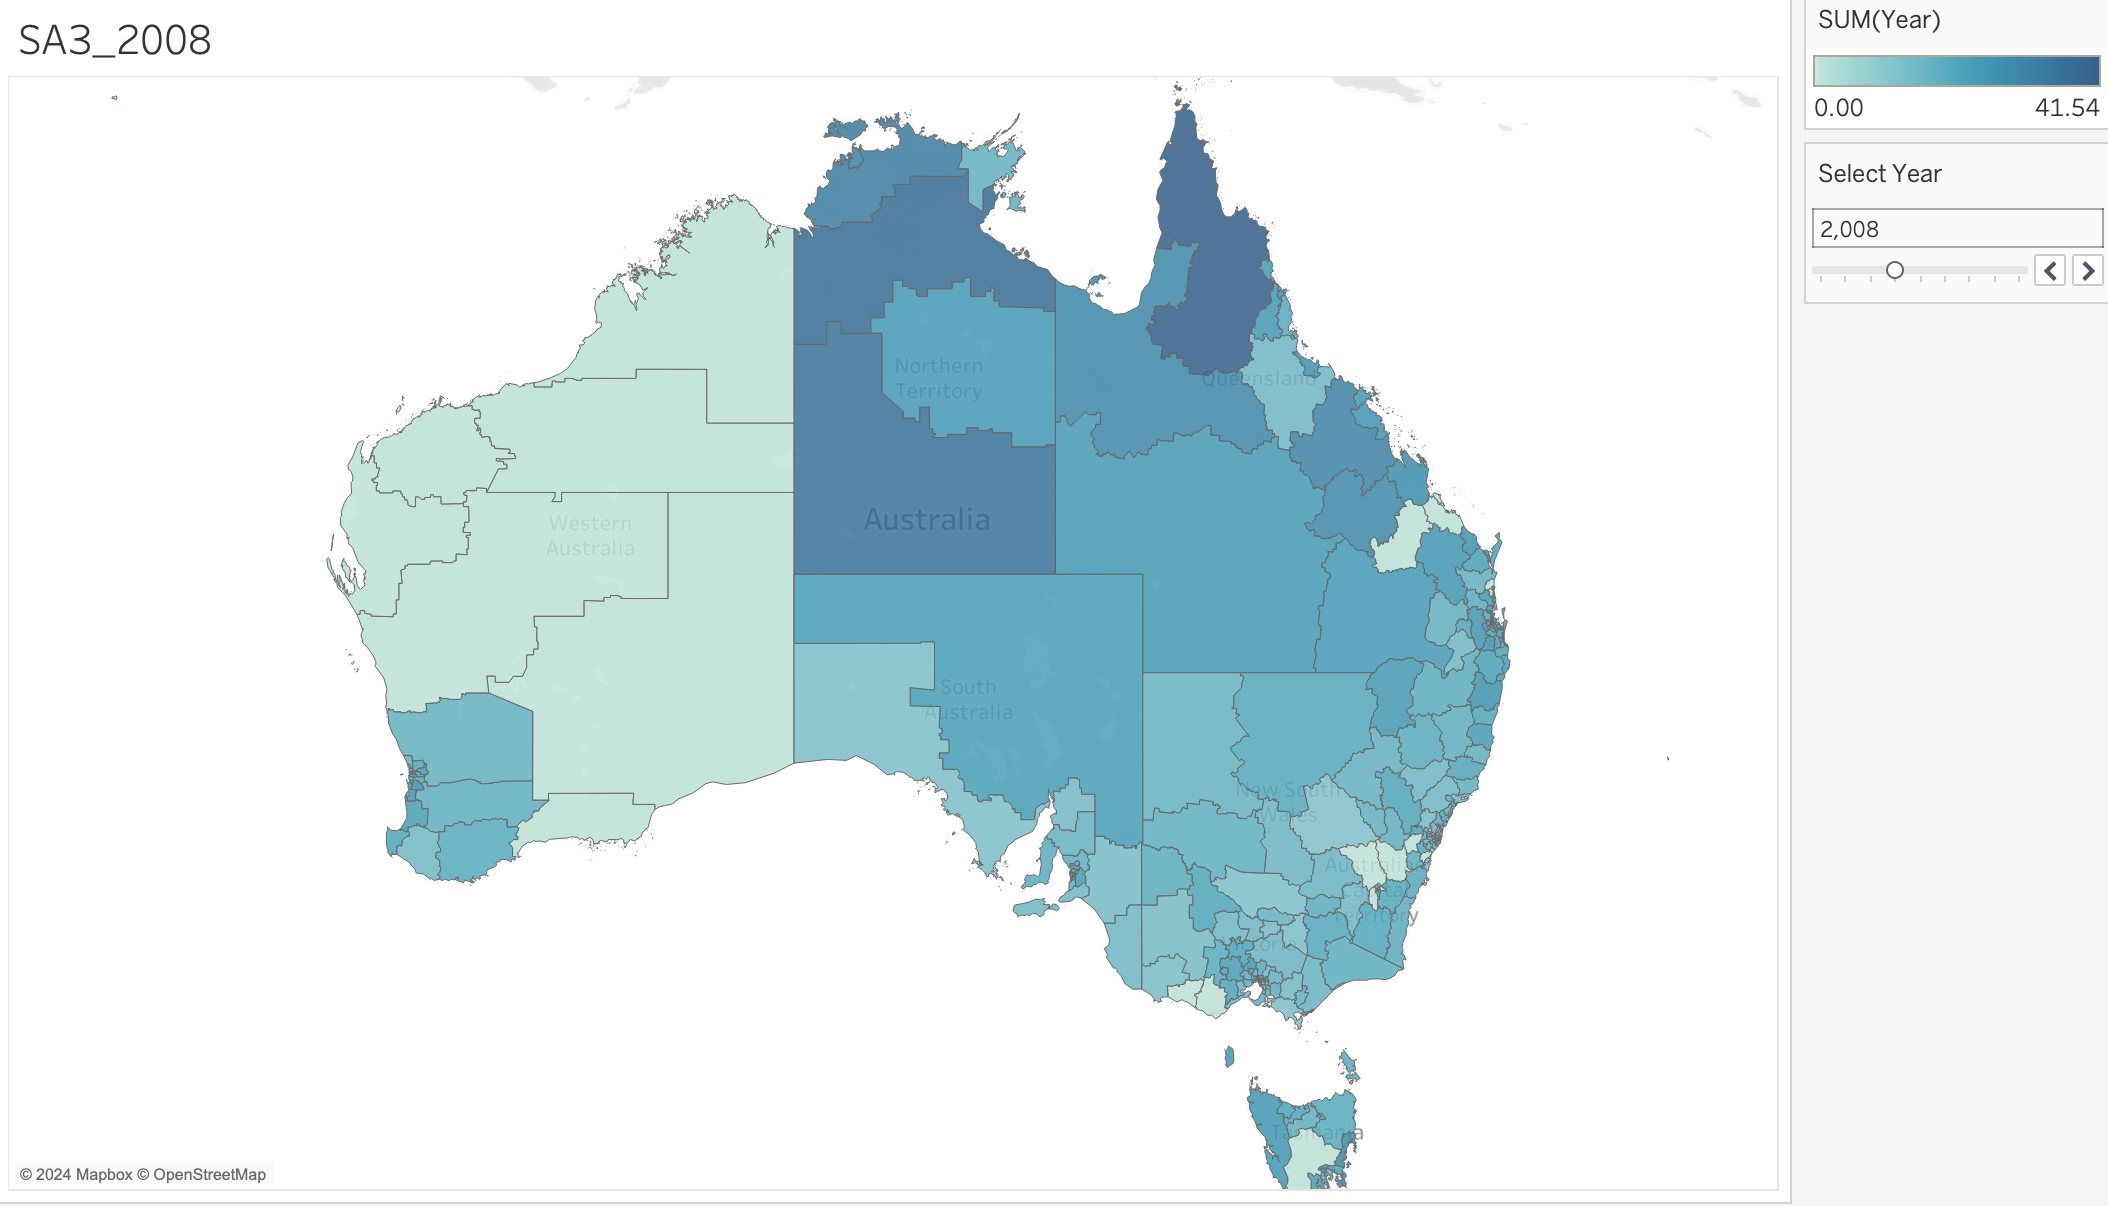
\includegraphics[width=0.45\textwidth]{images/Fig27.4.png}
        \label{fig:subfig4}
    }
    \hfill
    \subfloat[Heat map for 2009]{ 
        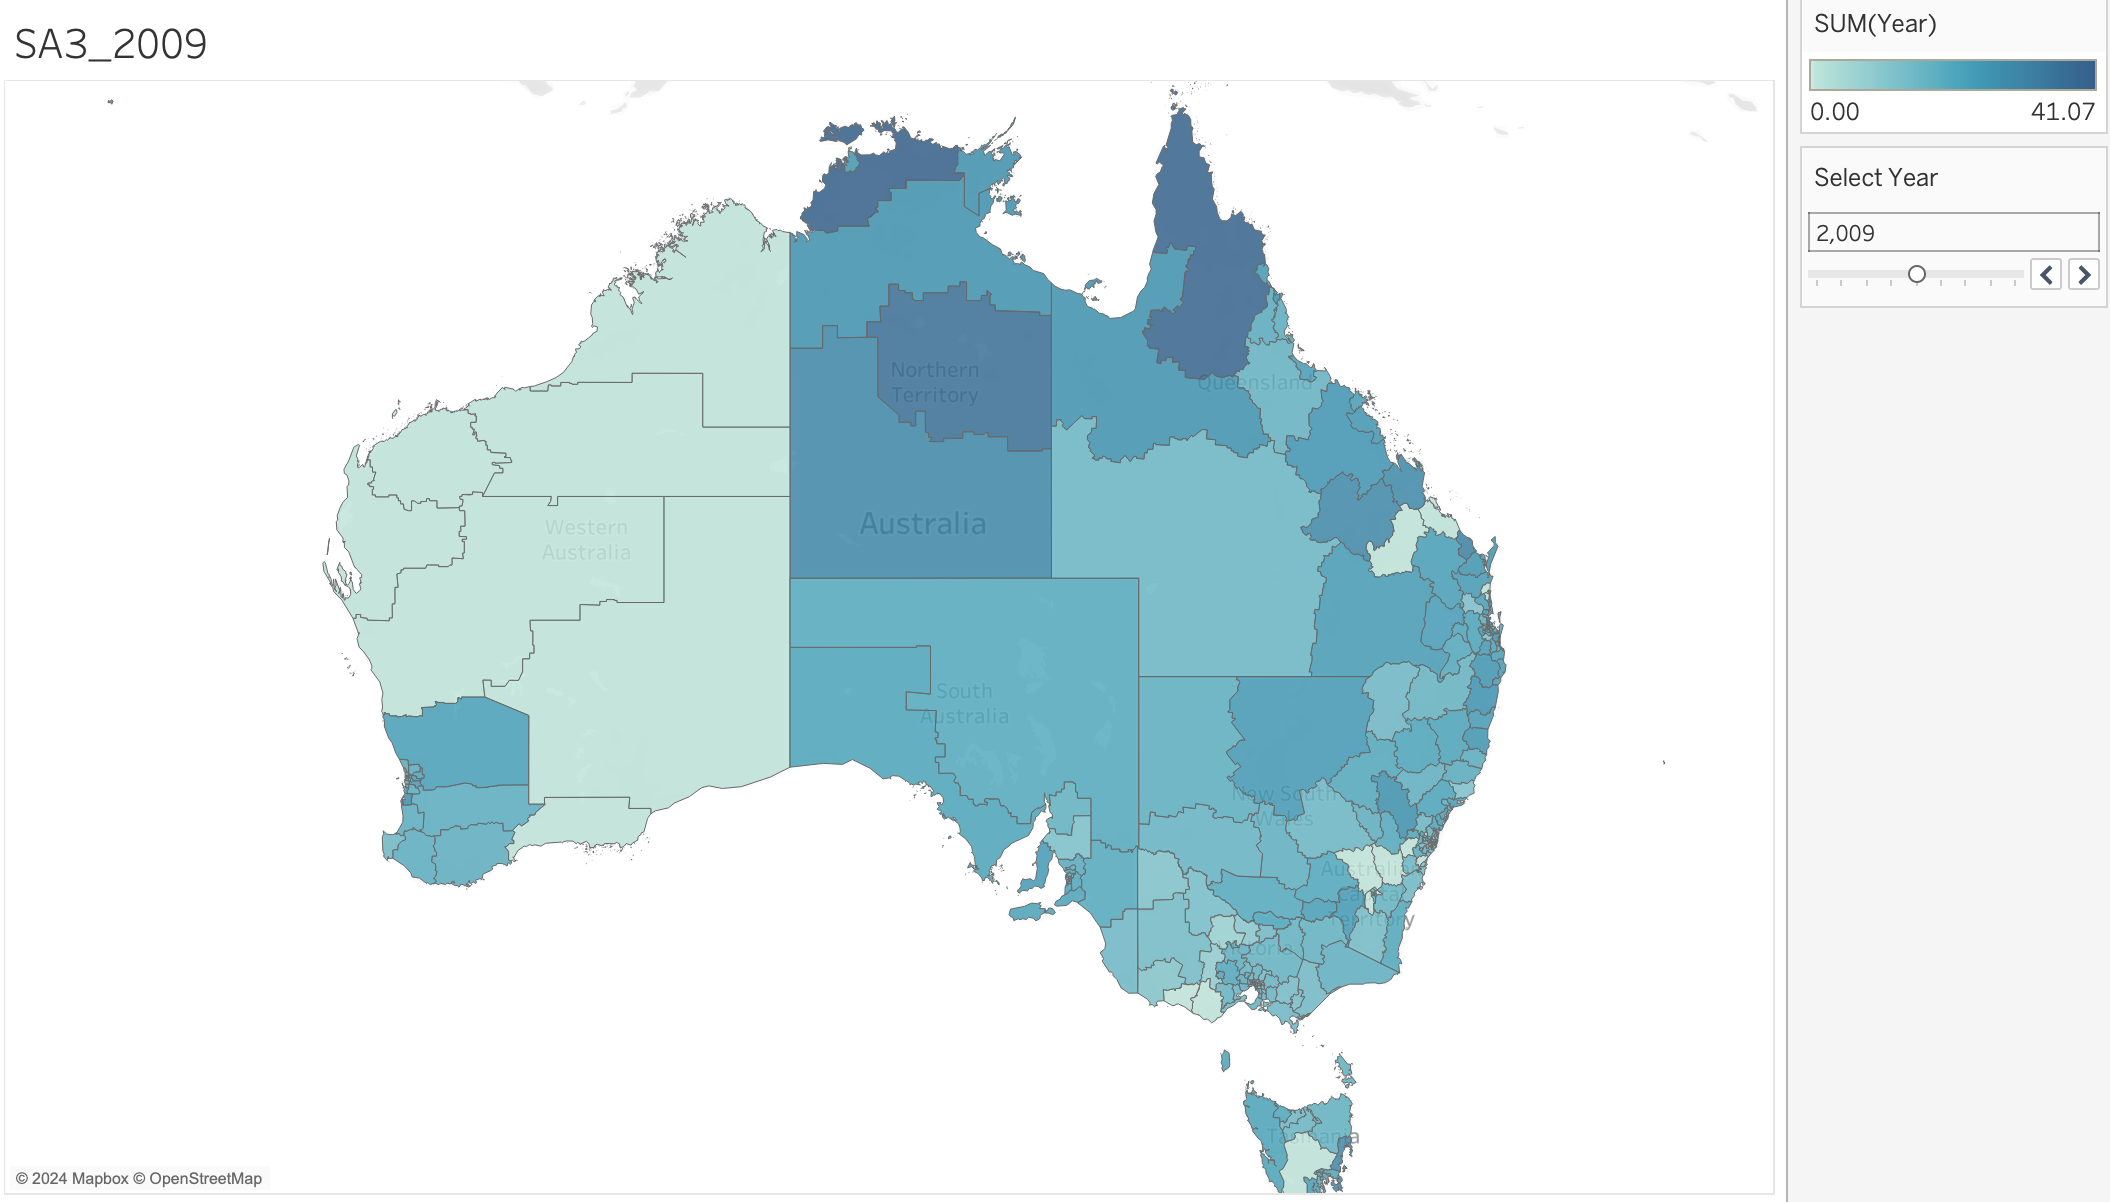
\includegraphics[width=0.45\textwidth]{images/Fig27.5.png}
        \label{fig:subfig5}
    }
    \vskip10pt
    \subfloat[Heat map for 2010]{ 
        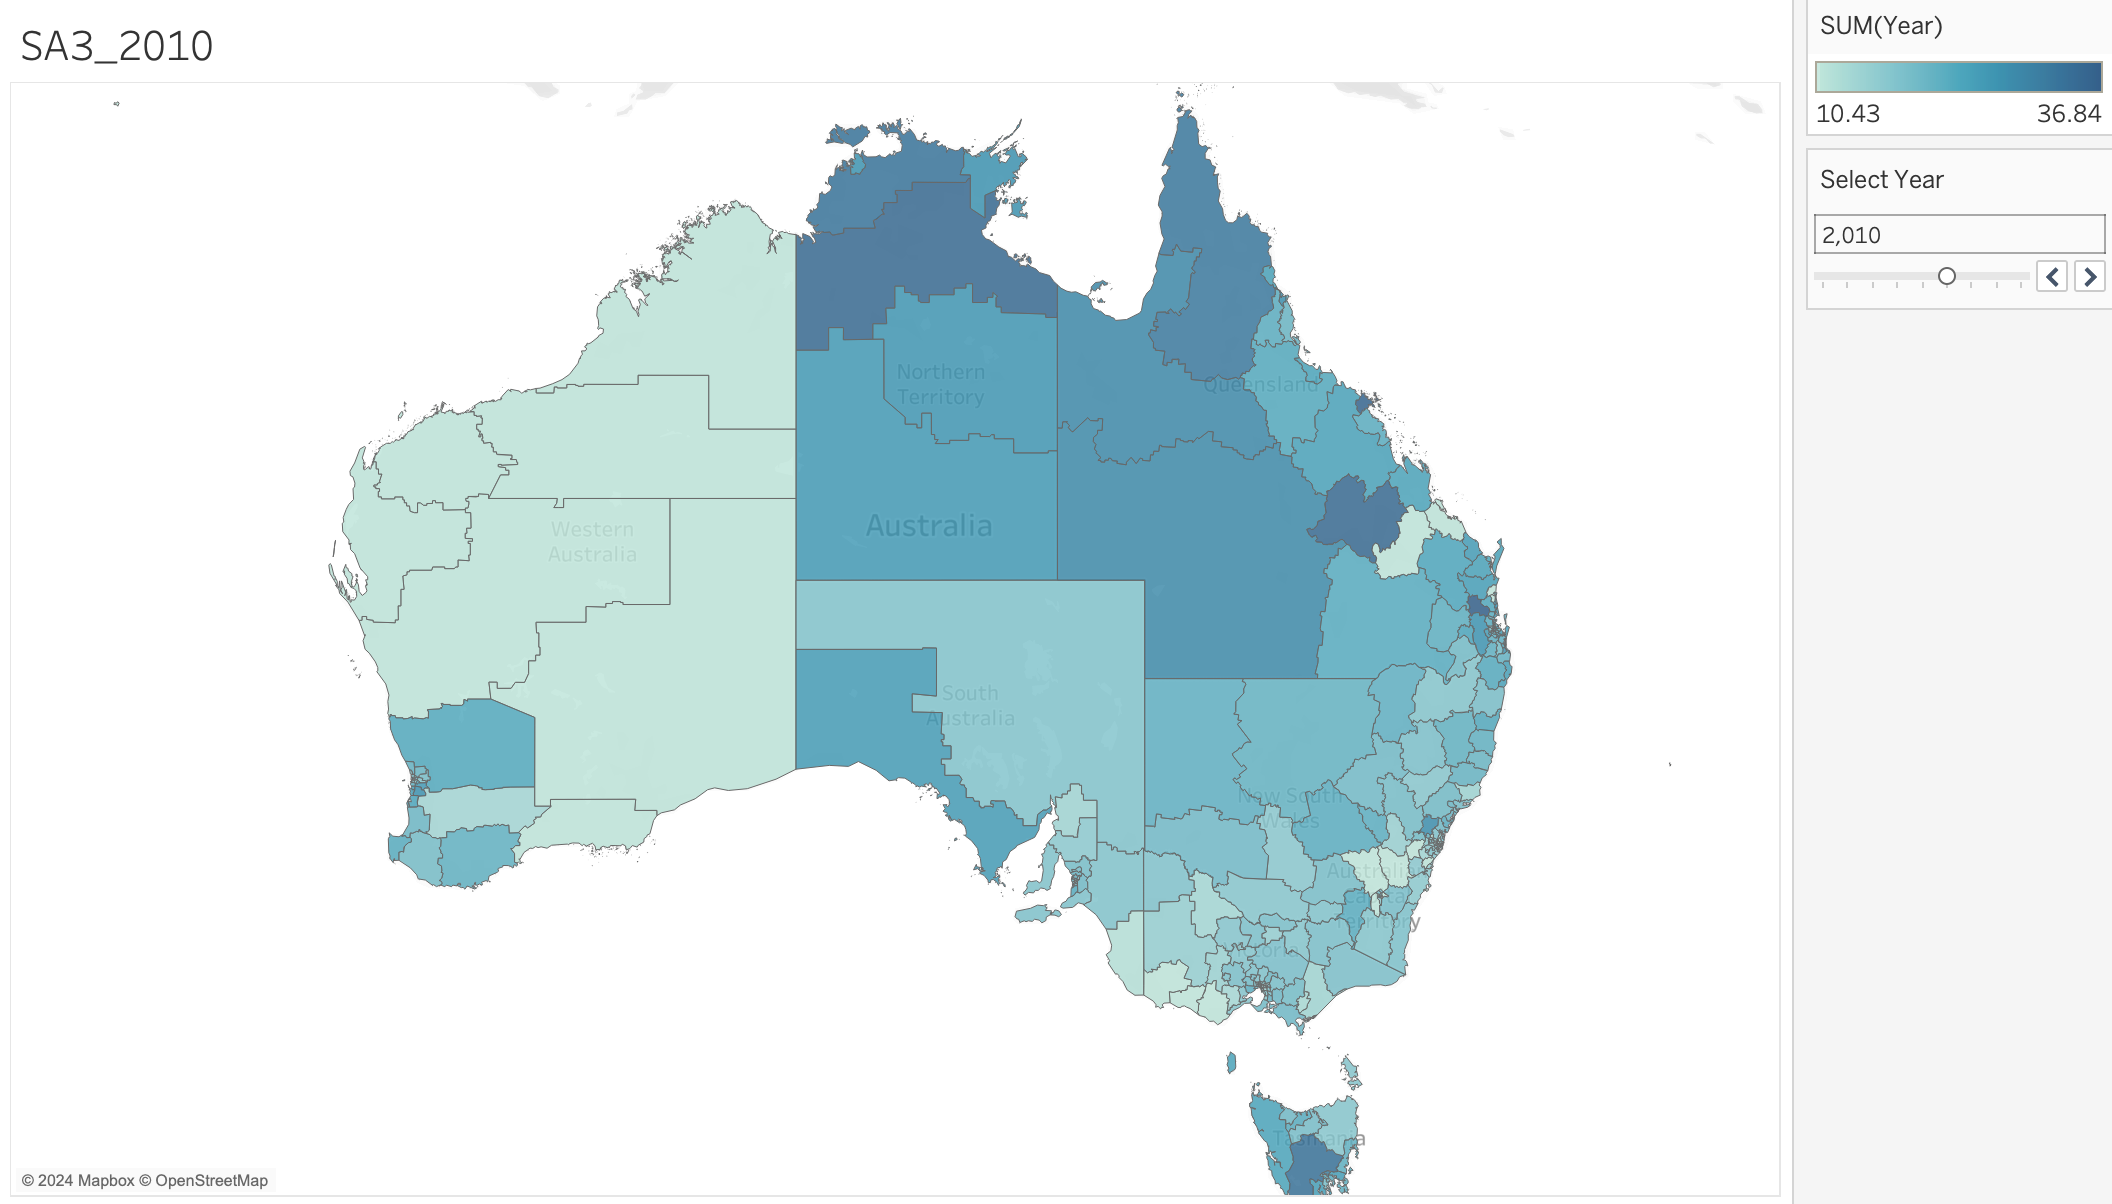
\includegraphics[width=0.45\textwidth]{images/Fig27.6.png}
        \label{fig:subfig6}
    }
    \hfill
    \subfloat[Heat map for 2011]{ 
        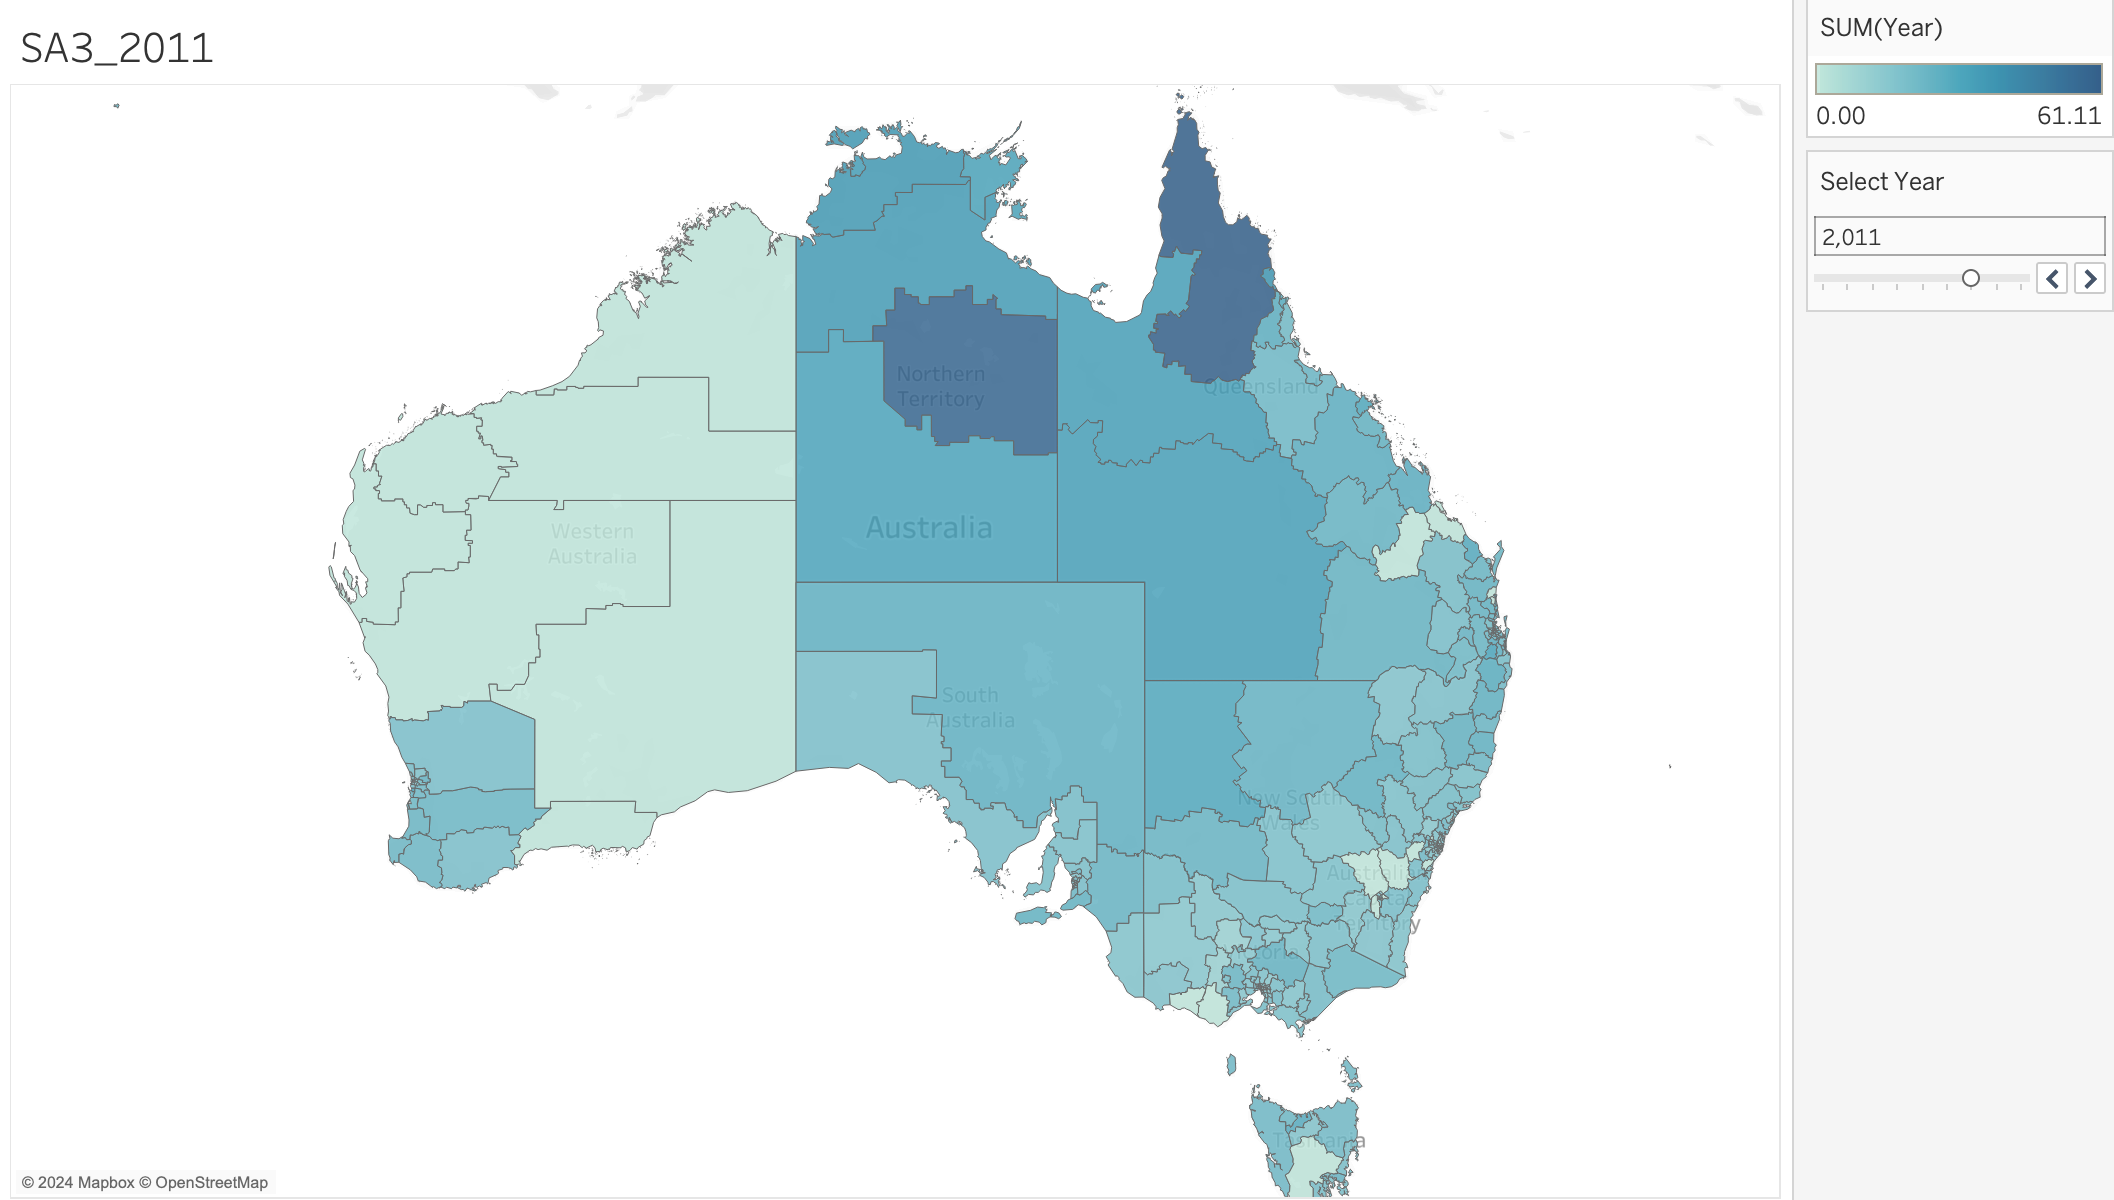
\includegraphics[width=0.45\textwidth]{images/Fig27.7.png}
        \label{fig:subfig7}
    }
    \vskip10pt
    \subfloat[Heat map for 2012]{ 
        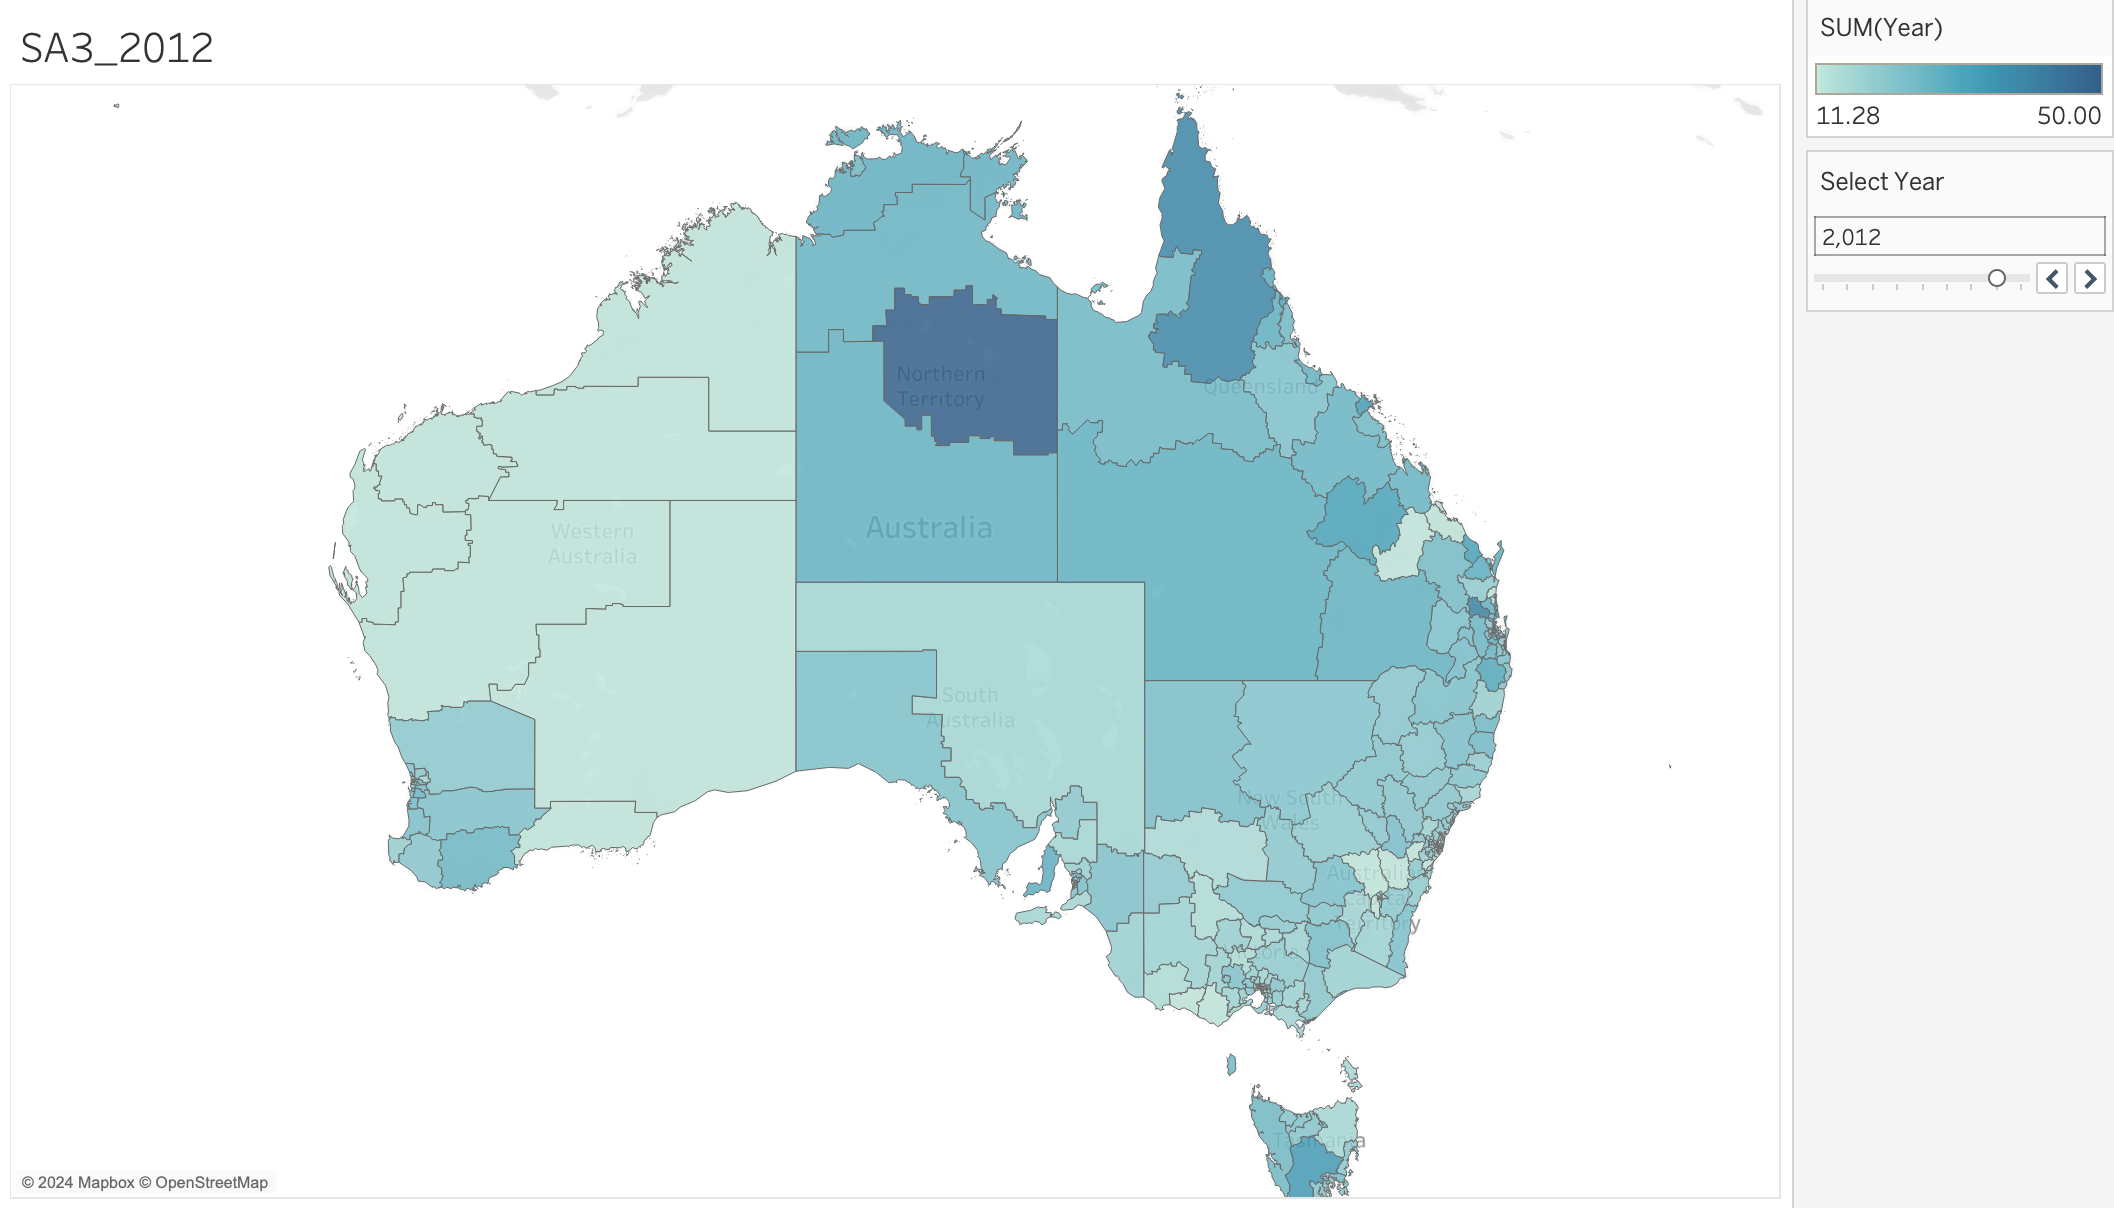
\includegraphics[width=0.45\textwidth]{images/Fig27.8.png}
        \label{fig:subfig8}
    }
    \hfill
    \subfloat[Heat map for 2013]{ 
        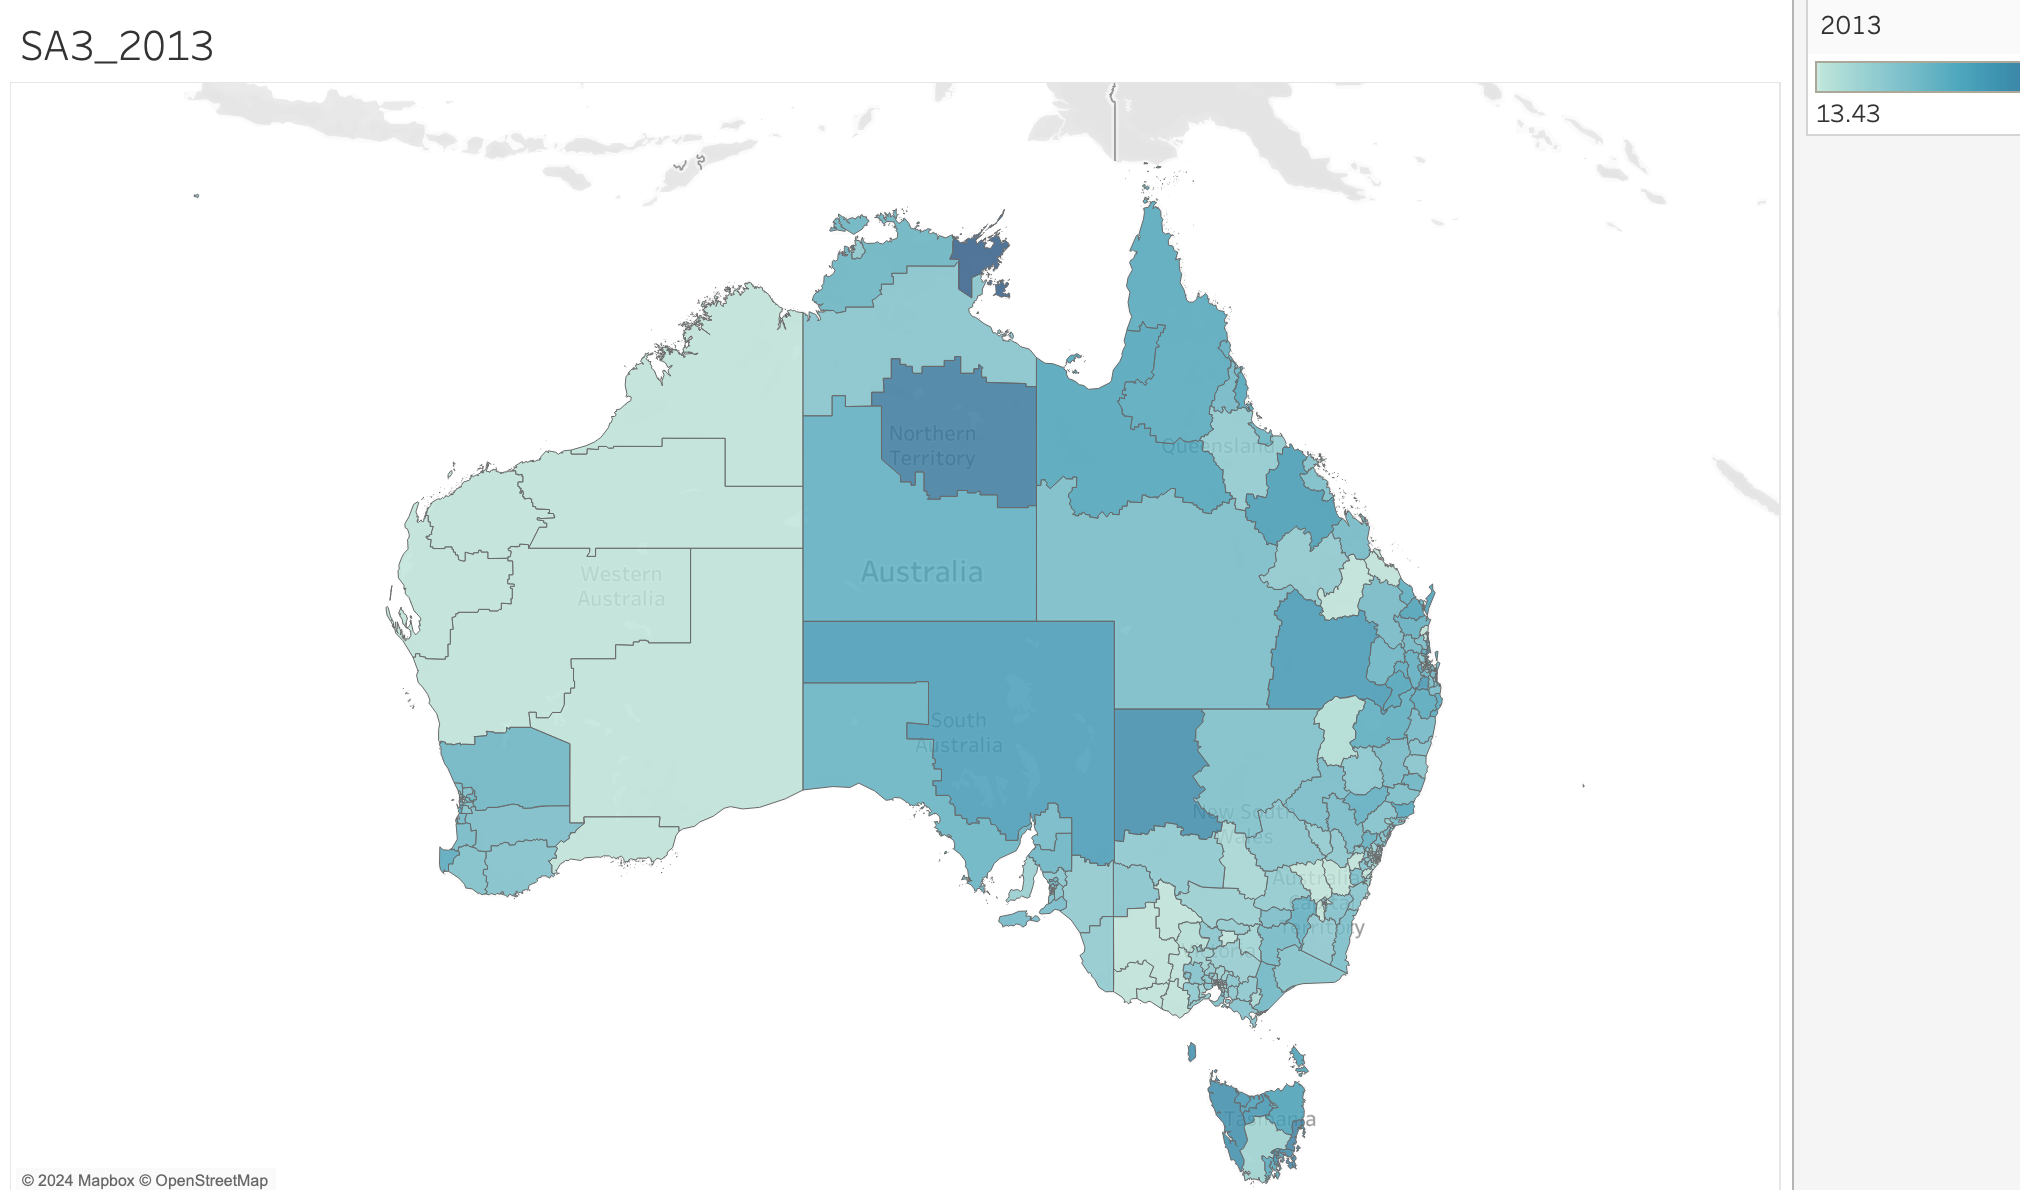
\includegraphics[width=0.45\textwidth]{images/Fig27.9.png}
        \label{fig:subfig9}
    }

    \caption{Heat maps for SA3 areas 2005 to 2013 (Part 2).}
    \label{fig:mainfigure2}
\end{figure*}
\clearpage



Key Observations and Insights: 
\begin{itemize} 
    \item Color Scheme: Darker teal shades represent higher attrition rates, and lighter shades indicate lower rates across the years (Figures \ref{fig:mainfigure1} and \ref{fig:mainfigure2}).
    \item Regional Trends: Northern regions, particularly in Queensland, consistently show darker shades, reflecting higher attrition rates. \item Southern and Western Regions: Southern regions exhibit lighter shades, indicating lower attrition. Western areas also appear lighter, likely due to imputed minimum attrition rates where data was missing.
    \item Attrition Stability: Minor variations in attrition rates are observed, but the overall distribution of high and low attrition regions remains stable across the years. 
    \item Heatmap Utility: The heatmaps effectively visualize the intensity of student attrition across regions, highlighting geographical and temporal patterns. 
    \item Color Choice: Teal is selected for its neutral and professional appearance, offering clear contrast between high and low attrition areas. 
\end{itemize}


\begin{figure}[H]
    \centering
    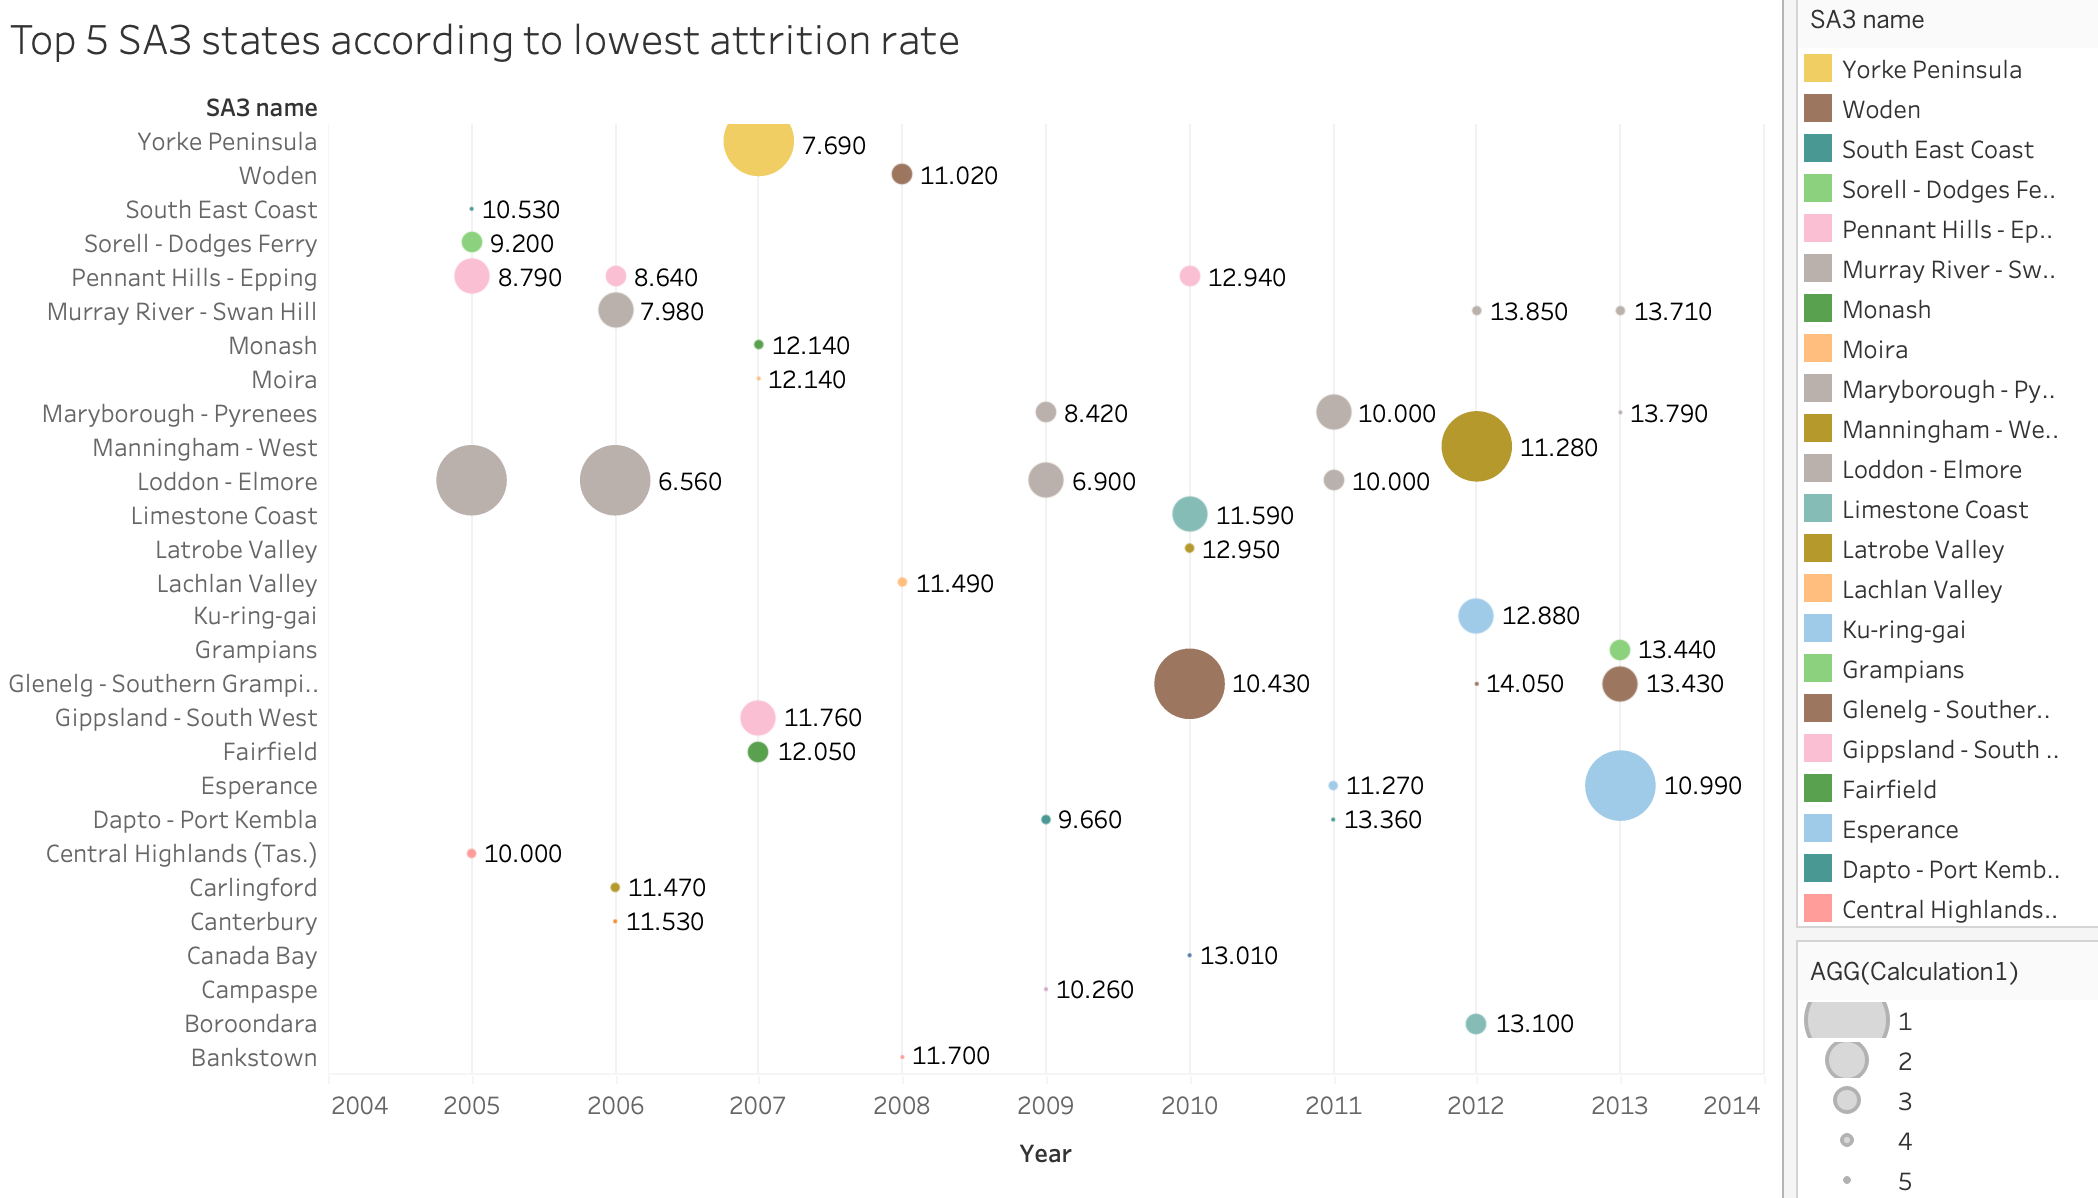
\includegraphics[width=0.4\textwidth]{images/Fig29.1.png}
    \caption{Scatter plot for top 5 states(based on SA3) with lowest attrition rate across years.}
    \label{fig:bubble1}
\end{figure}
\begin{figure}[H]
    \centering
    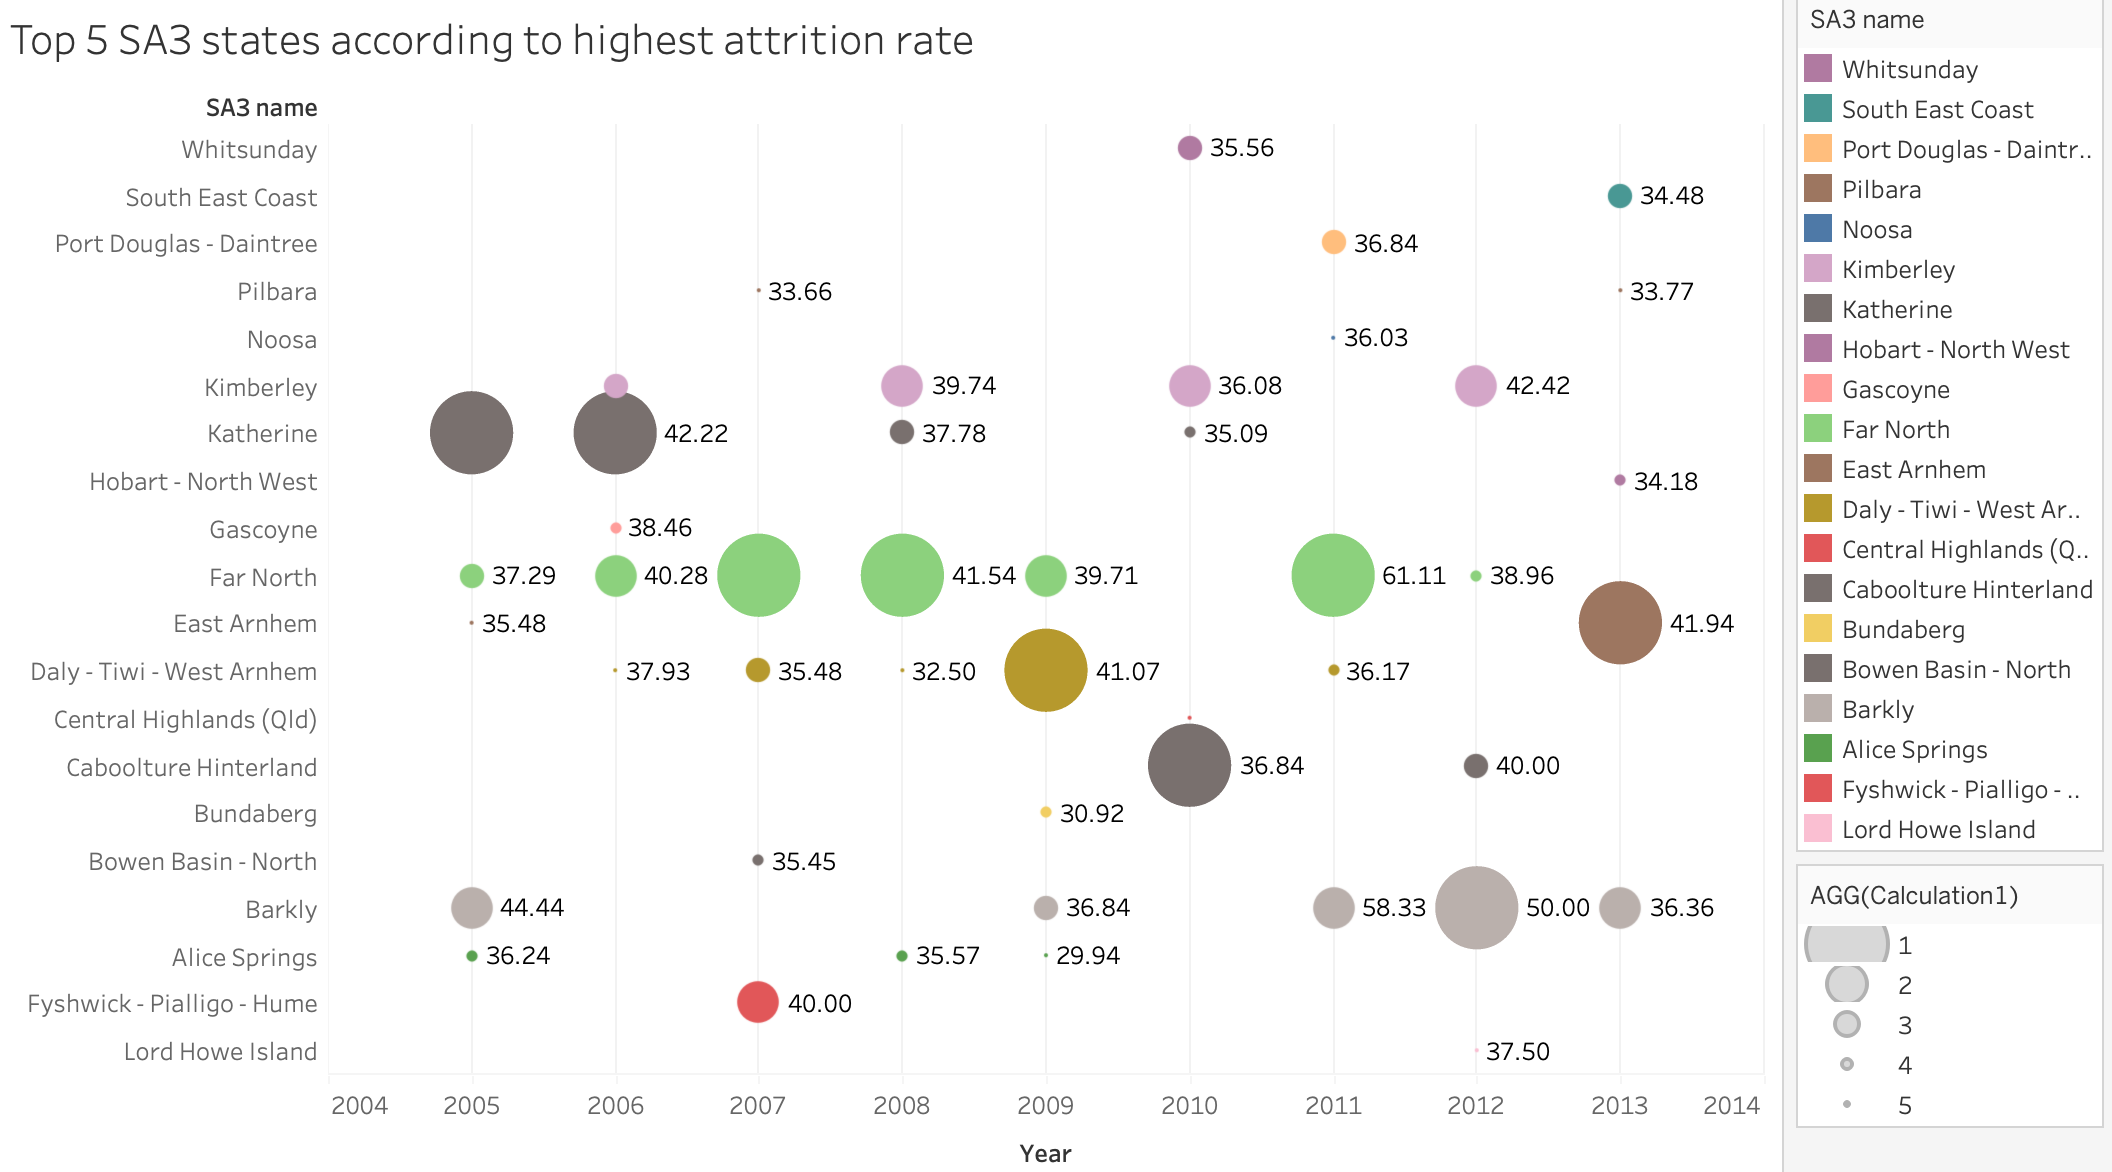
\includegraphics[width=0.4\textwidth]{images/Fig29.2.png}
    \caption{Scatter plot for top 5 states(based on SA3) with highest attrition rate across years.}
    \label{fig:bubble2}
\end{figure}

We have plotted bubble charts (Figures \ref{fig:bubble1} and \ref{fig:bubble2}) to visualize the top 5 states with the highest and lowest attrition rates across different years for SA3 regions. Key observations and insights are:
\begin{itemize} 
    \item Figures \ref{fig:bubble1} and \ref{fig:bubble2} use circle size to represent attrition rates. Larger circles indicate regions with the highest or lowest attrition rates, while smaller circles represent regions with intermediate rates.
    \item Figure \ref{fig:bubble1} displays the top 5 states with the lowest attrition rates across years. Regions like Loddon-Elmore (grey), Glenelg-Southern (brown), and Murray River (pink) consistently appear on the map, indicating their lower attrition rates over time. In 2013, the states with the lowest rates are Esperance (10.99\%), Glenelg-Southern (13.43\%), Grampians (13.44\%), Murray River-Swan Hill (13.71\%), and Marlborough-Pyrenees (13.79\%). 
    \item Figure \ref{fig:bubble2} shows the top 5 states with the highest attrition rates across years. Regions such as Far North (light green), Barkly (grey), and Kimberley (light purple) frequently appear, indicating consistently high attrition rates. In 2013, the states with the highest rates are East Arnhem (41.94\%), Barkly (36.36\%), Port Douglas (34.38\%), Hobart-North West (34.18\%), and Pilbara (33.77\%). 
    \item The bubble charts ensure that the size of the circles is proportional to the attrition rates, making it easy to identify regions with the highest and lowest rates. Larger circles stand out clearly. 
\end{itemize}
\par
\vspace{10pt}
\subsubsection{Based on LGA area analysis:}
Figure \ref{fig:mainfigure3} and \ref{fig:mainfigure4} shows different heat map for attrition rate across different years from 2005-2013 according to LGA regions of Australia.

\par
\vspace{10pt}

\begin{figure}[H]
    % First row of subfigures
    \centering
    \subfloat[Heat map for 2005]{ % Manually manage the numbering
        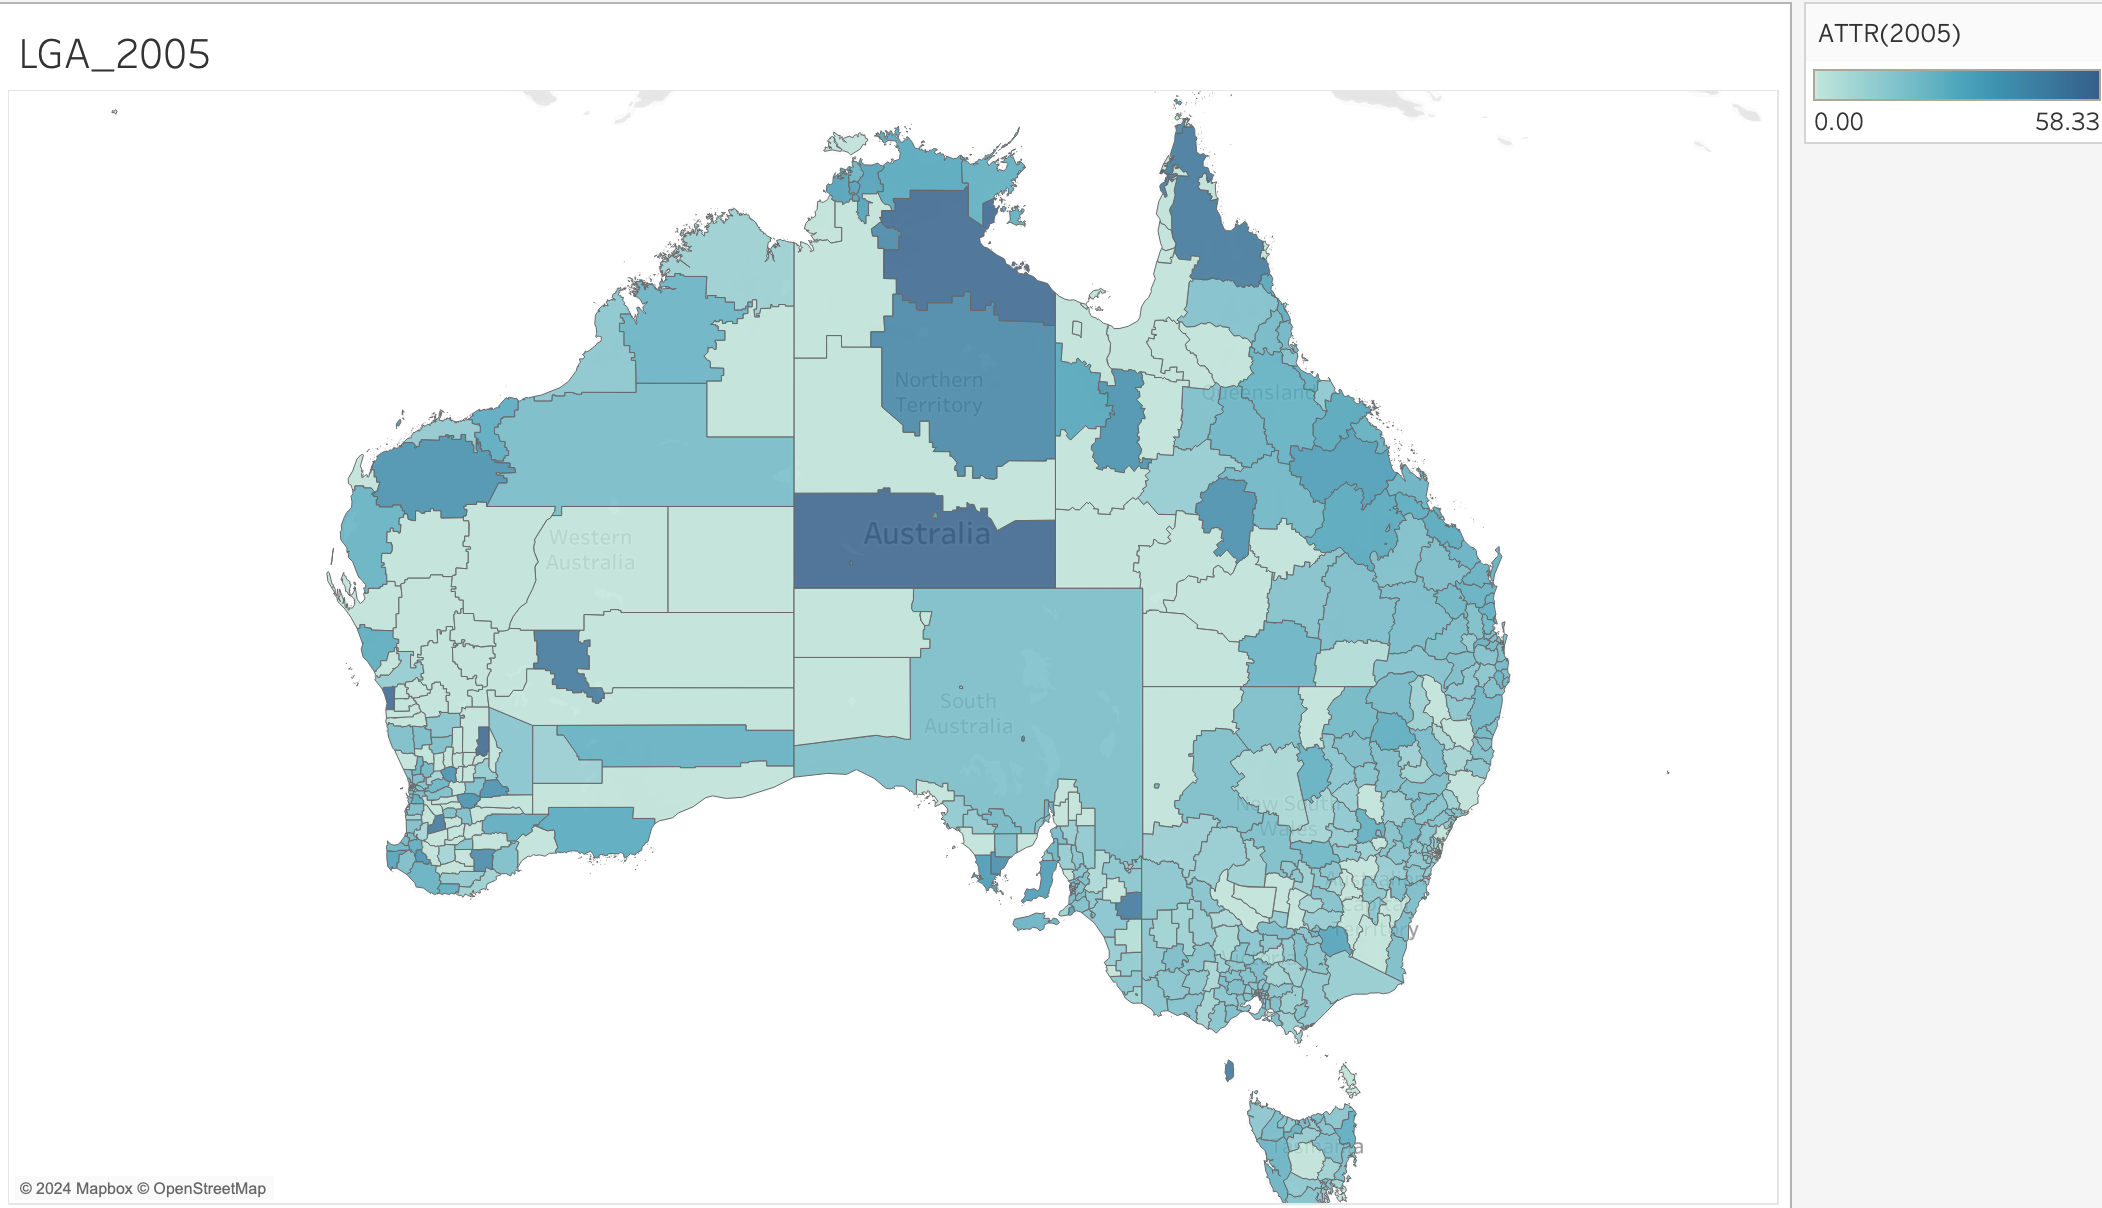
\includegraphics[width=0.45\textwidth]{images/Fig30.1.png}
        \label{fig:subfig10}
    }
    \vskip5pt
    \subfloat[Heat map for 2006]{ % Continue numbering from the previous figure
        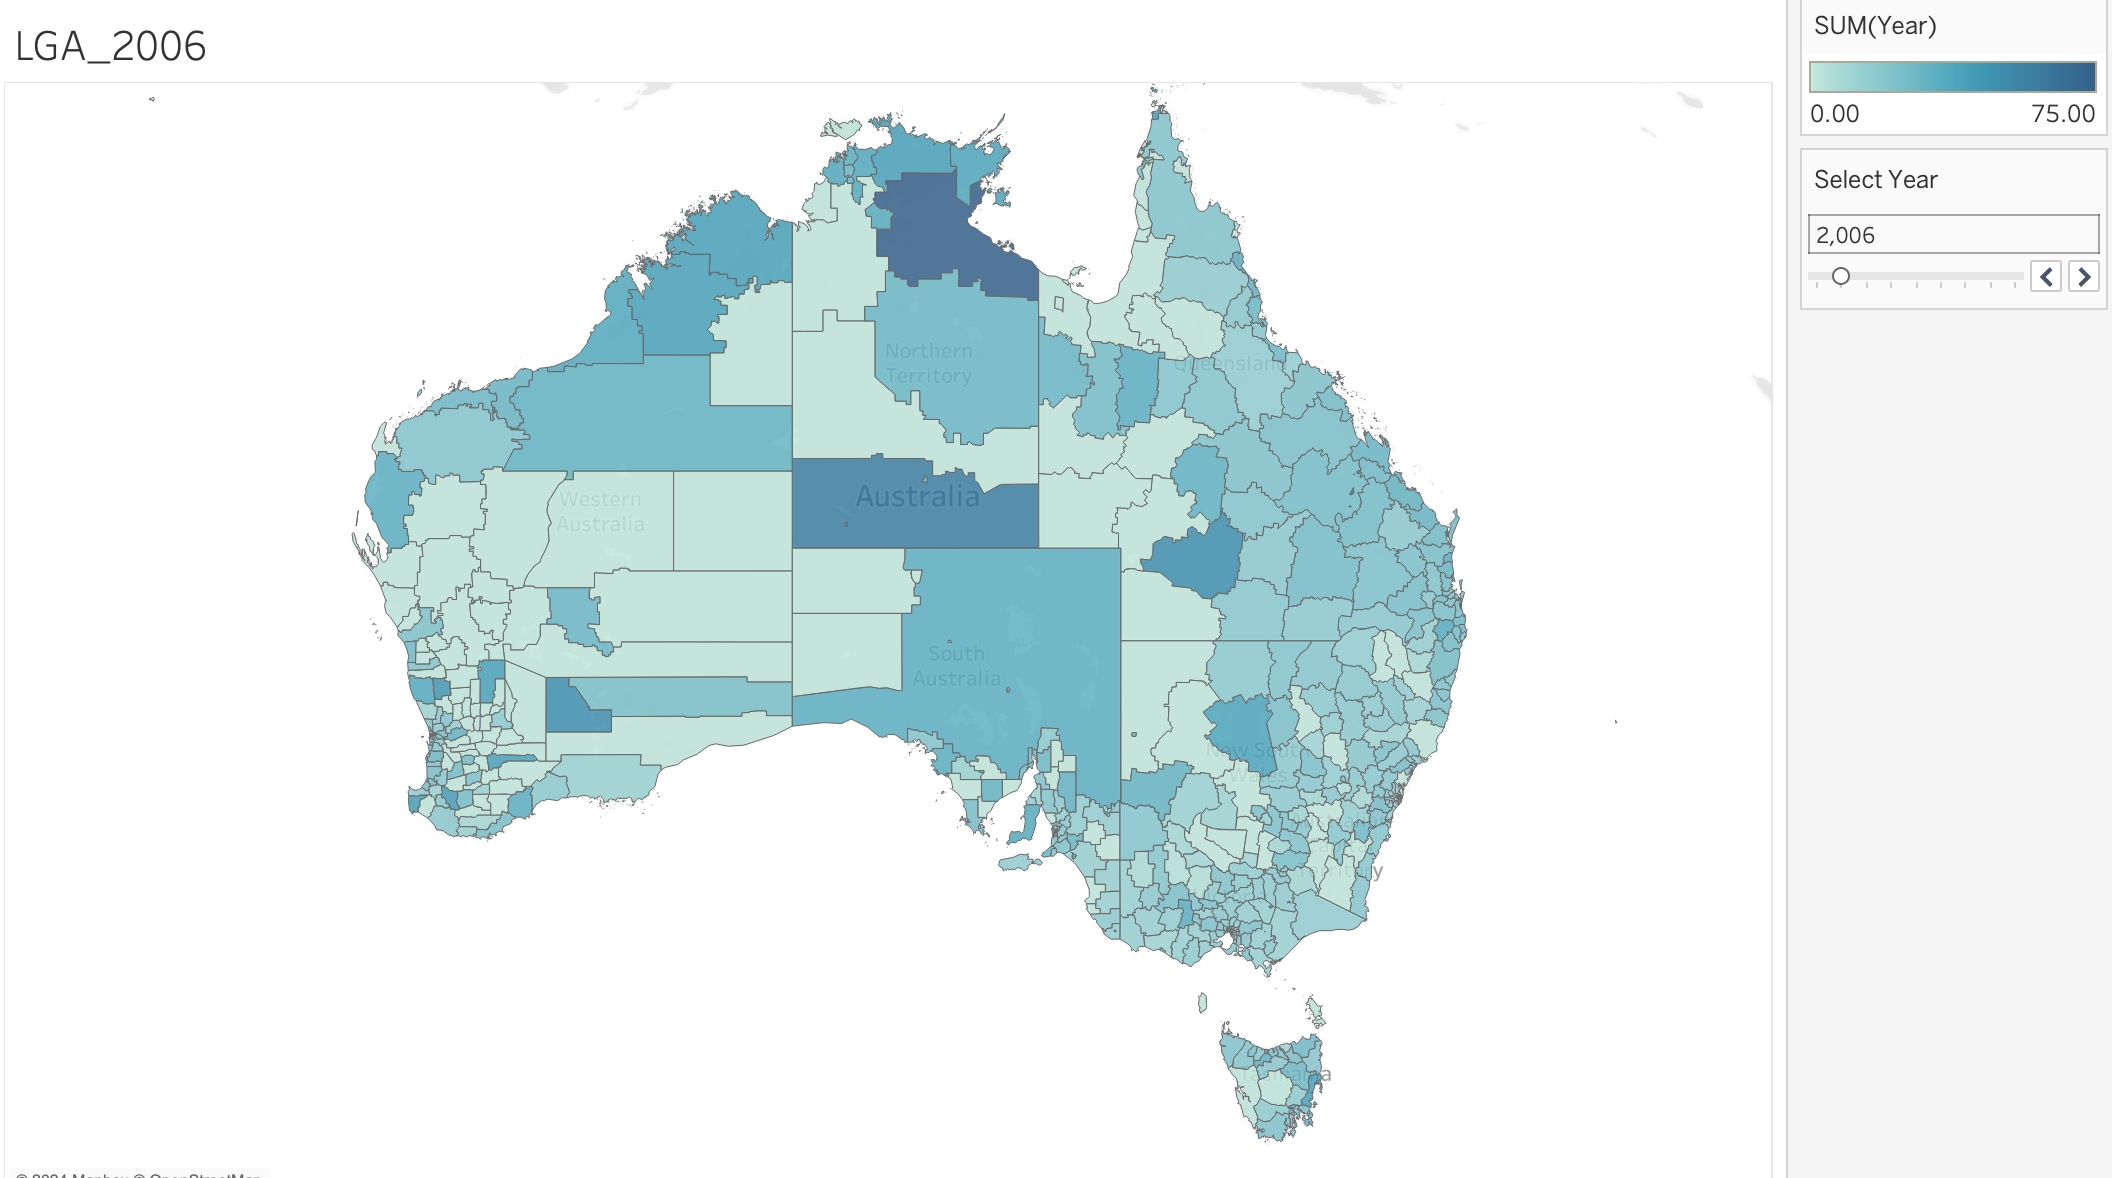
\includegraphics[width=0.45\textwidth]{images/Fig30.2.png}
        \label{fig:subfig11}
    }
    \vspace{10pt}
    \caption{Heat maps for LGA areas 2005 to 2013 (Part 1).}
    \label{fig:mainfigure3}
\end{figure}

\clearpage
\begin{figure*}[tb]
    % Second row of subfigures
    
    \subfloat[Heat map for 2007]{ % Continue numbering from the previous figure
        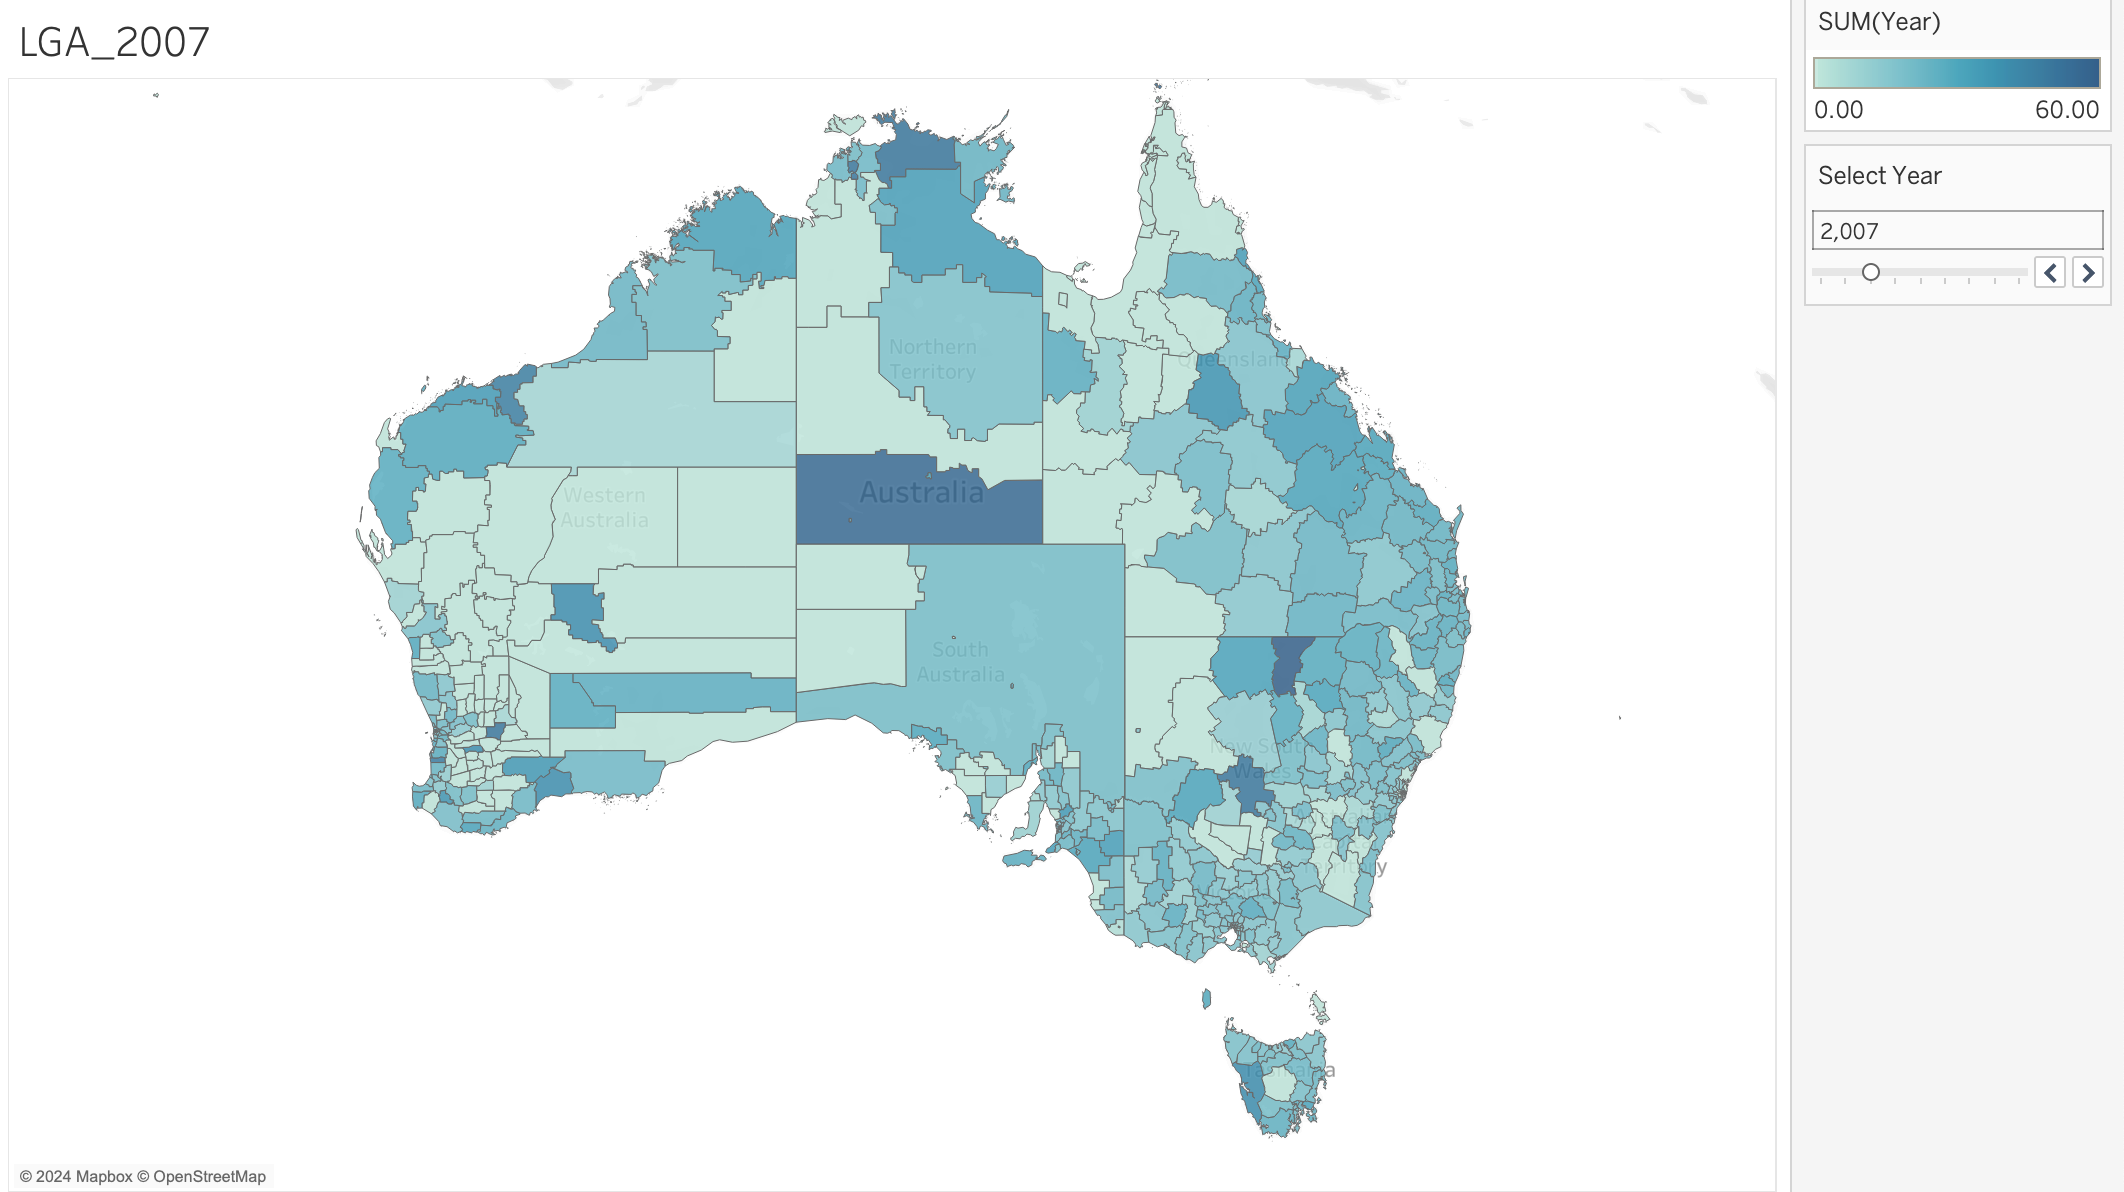
\includegraphics[width=0.45\textwidth]{images/Fig30.3.png}
        \label{fig:subfig12}
    }
    \hfill
    \subfloat[Heat map for 2008]{ 
        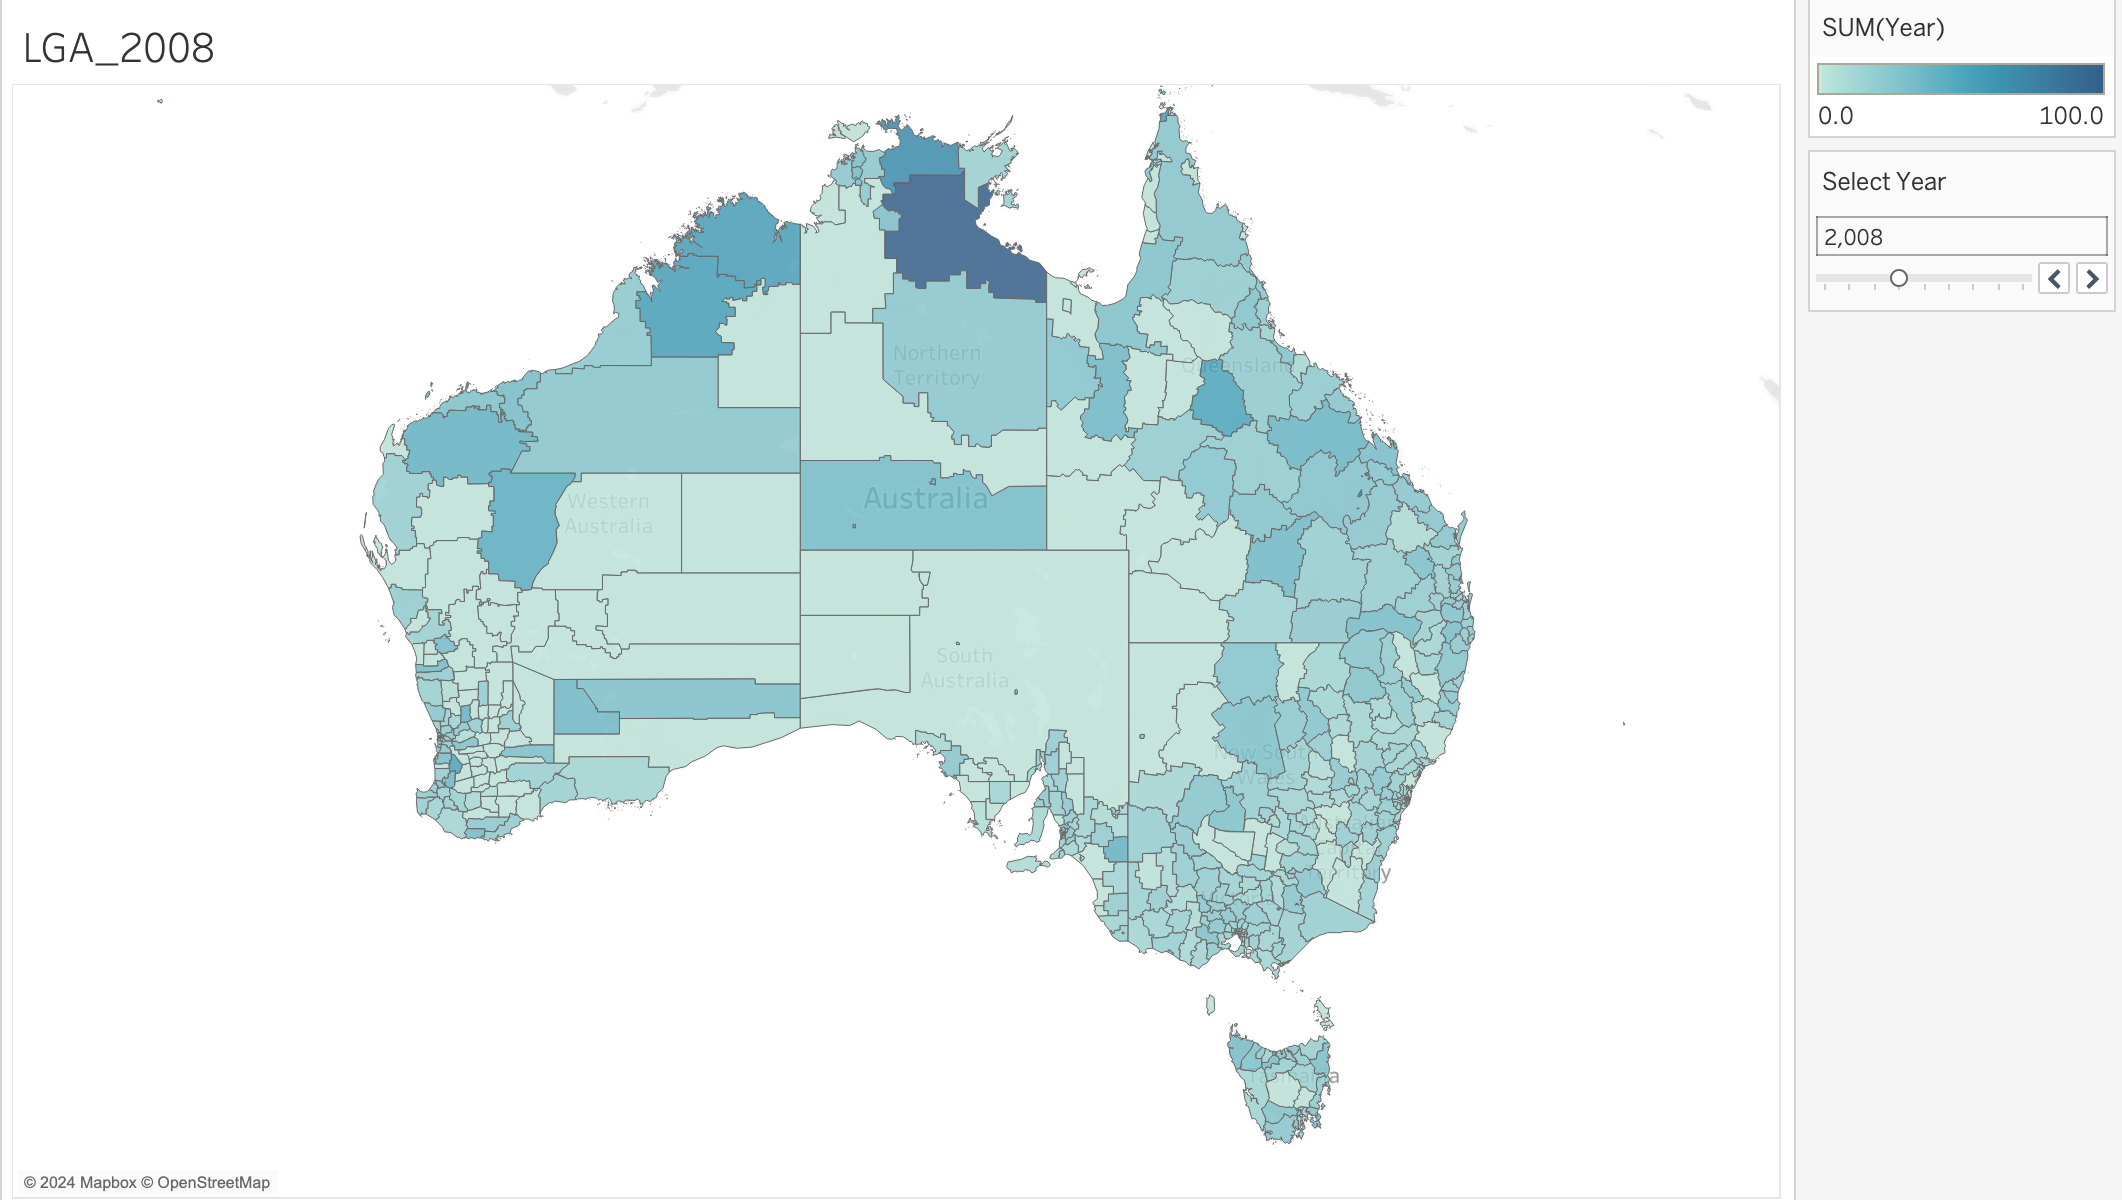
\includegraphics[width=0.45\textwidth]{images/Fig30.4.png}
        \label{fig:subfig13}
    }
    \vskip10pt
    \subfloat[Heat map for 2009]{ 
        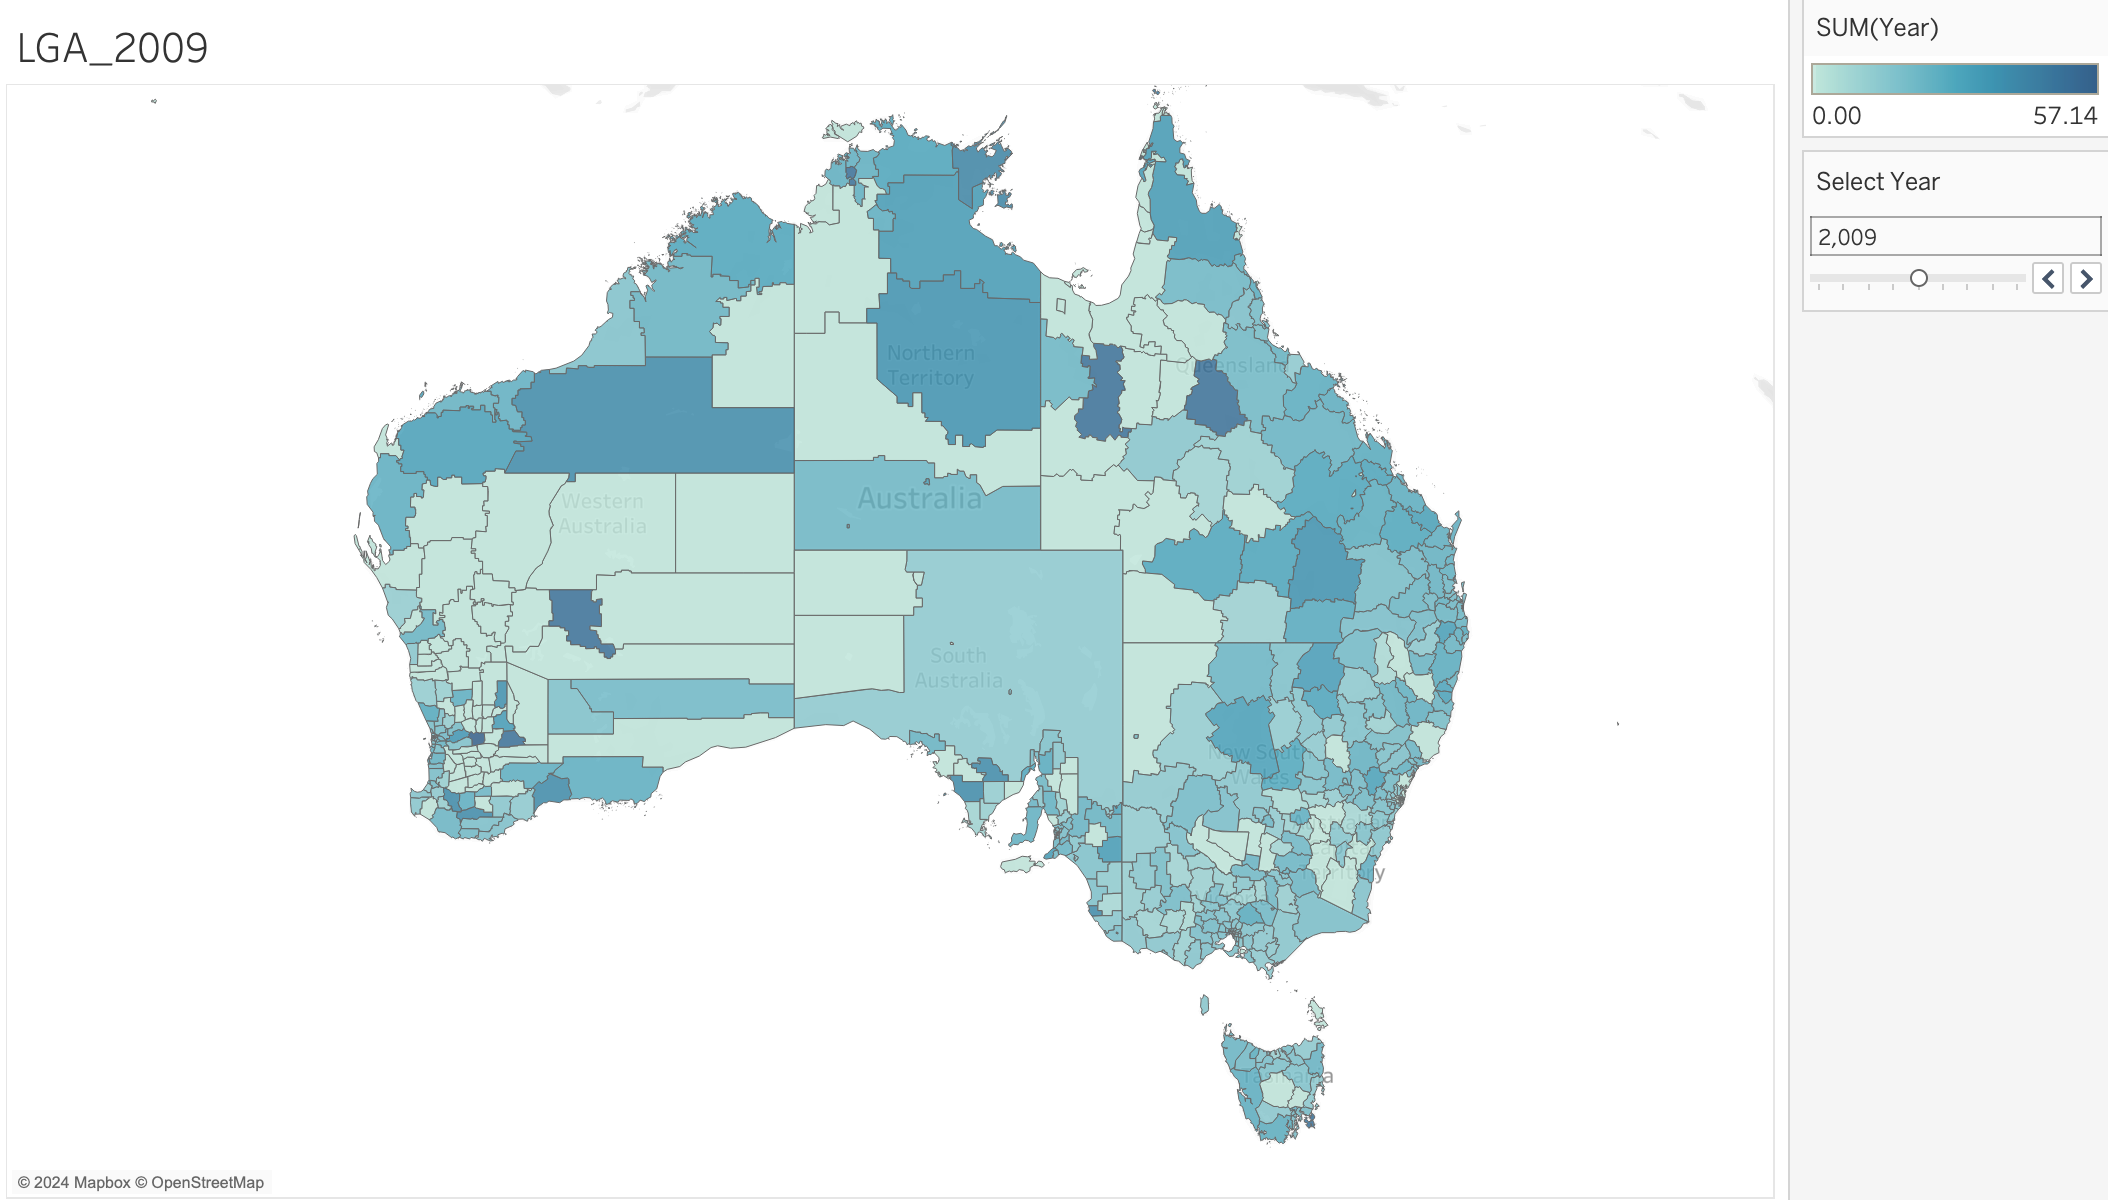
\includegraphics[width=0.45\textwidth]{images/Fig30.5.png}
        \label{fig:subfig14}
    }
    \hfill
    \subfloat[Heat map for 2010]{ 
        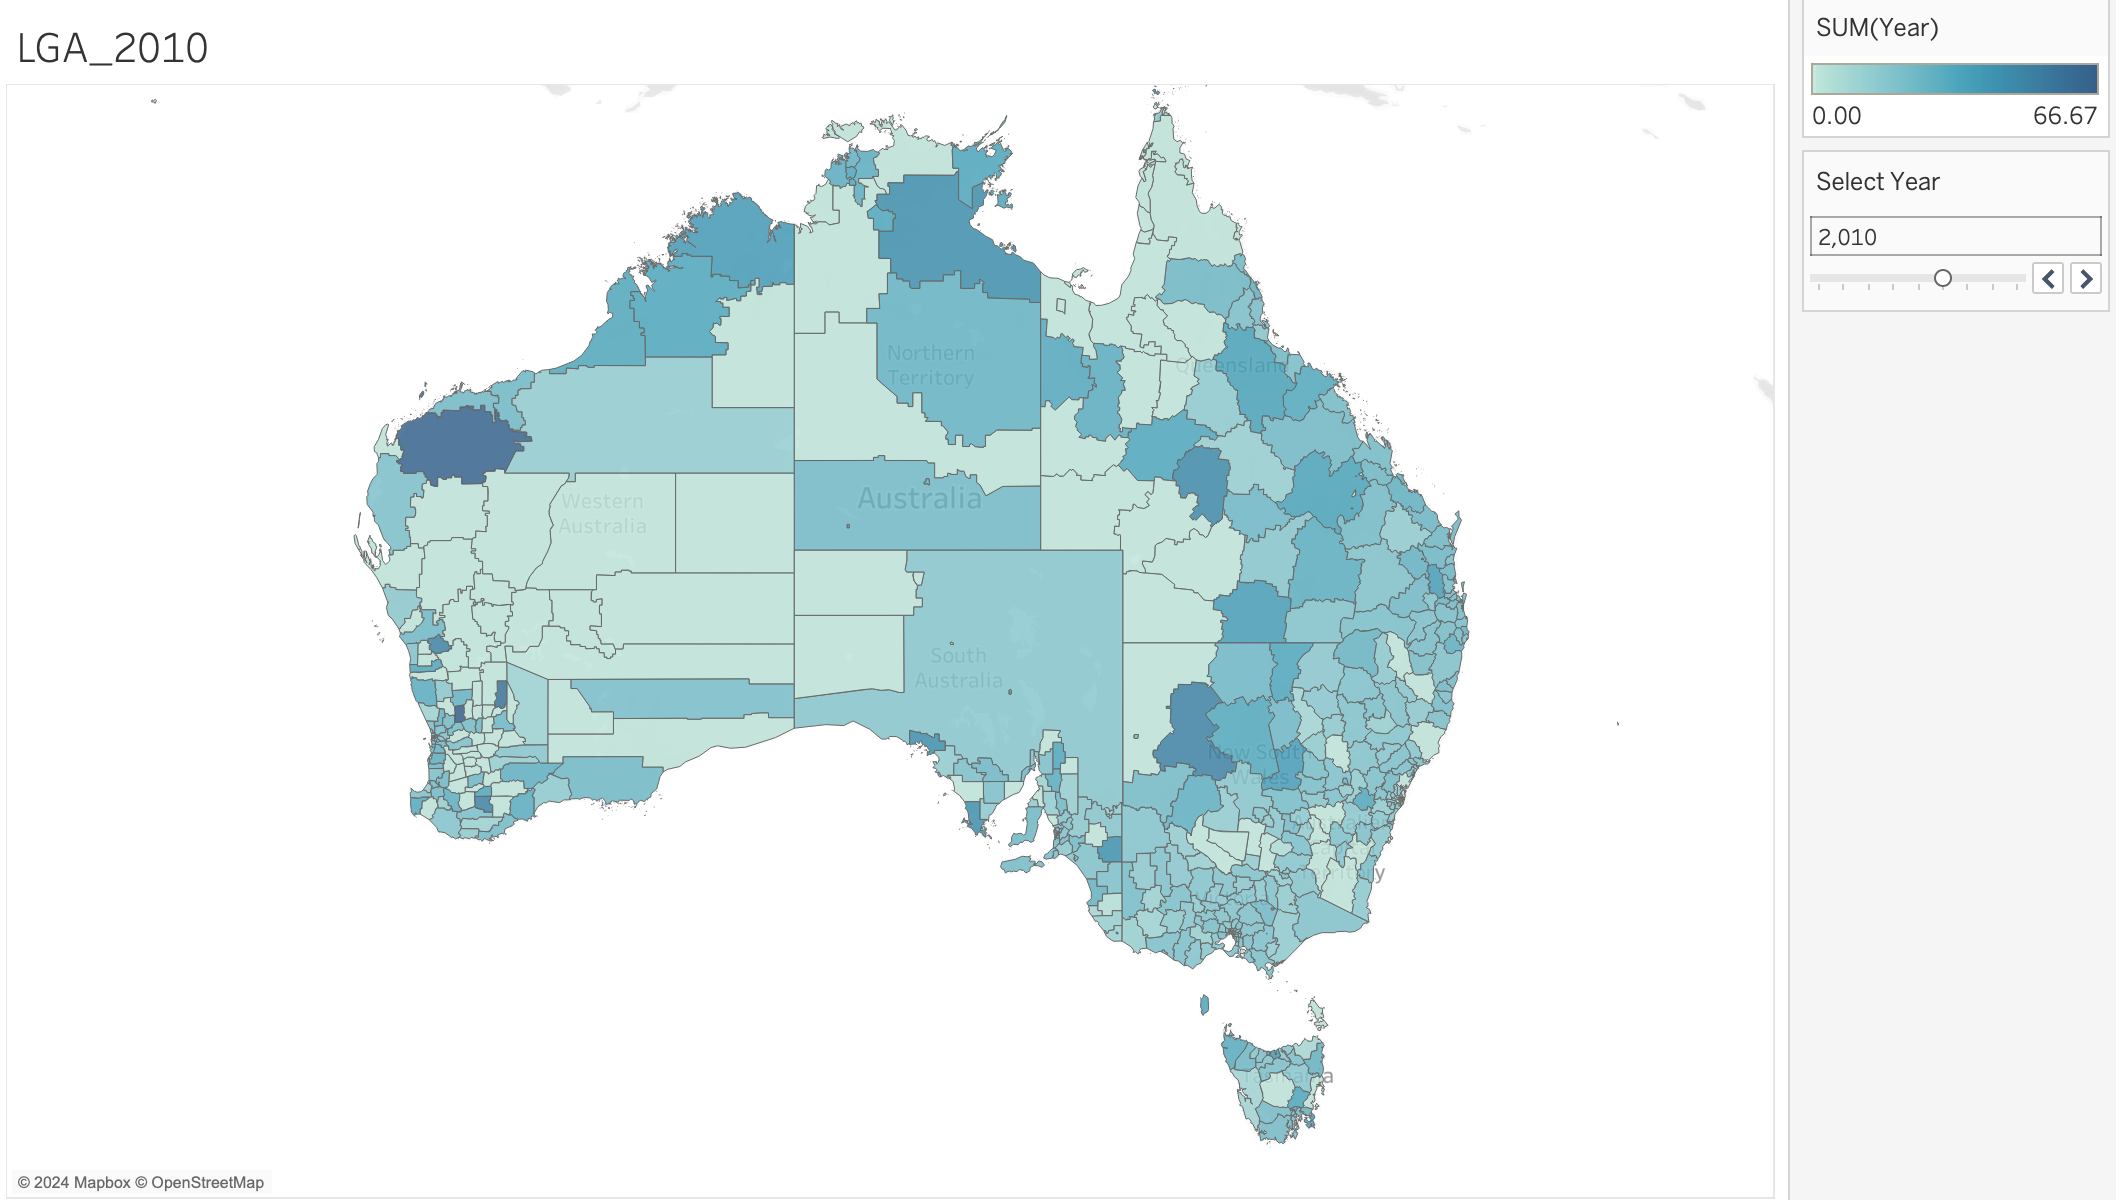
\includegraphics[width=0.45\textwidth]{images/Fig30.6.png}
        \label{fig:subfig15}
    }
    \vskip10pt
    \subfloat[Heat map for 2011]{ 
        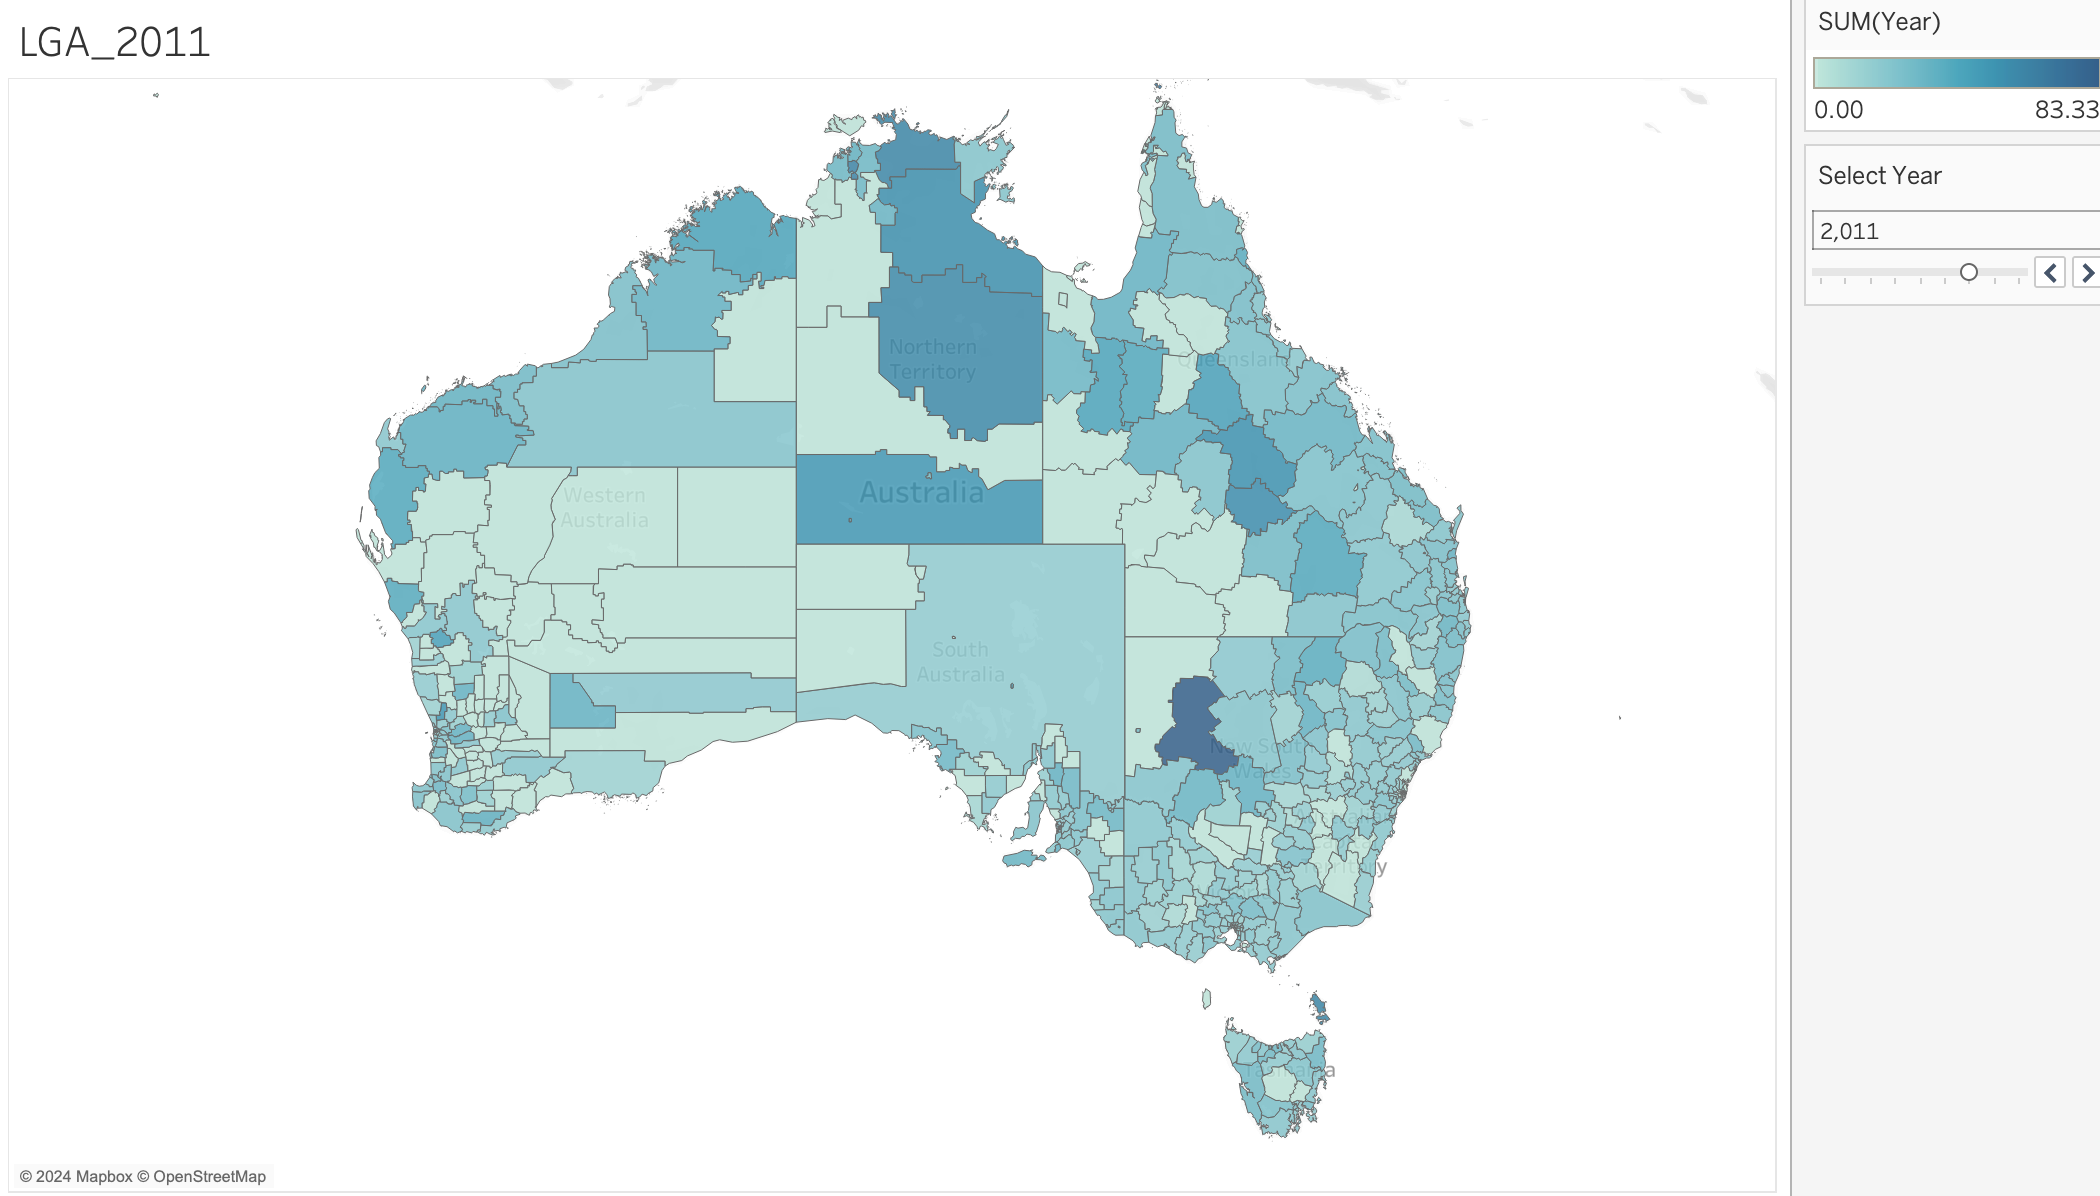
\includegraphics[width=0.45\textwidth]{images/Fig30.7.png}
        \label{fig:subfig16}
    }
    \hfill
    \subfloat[Heat map for 2012]{ 
        \centering
        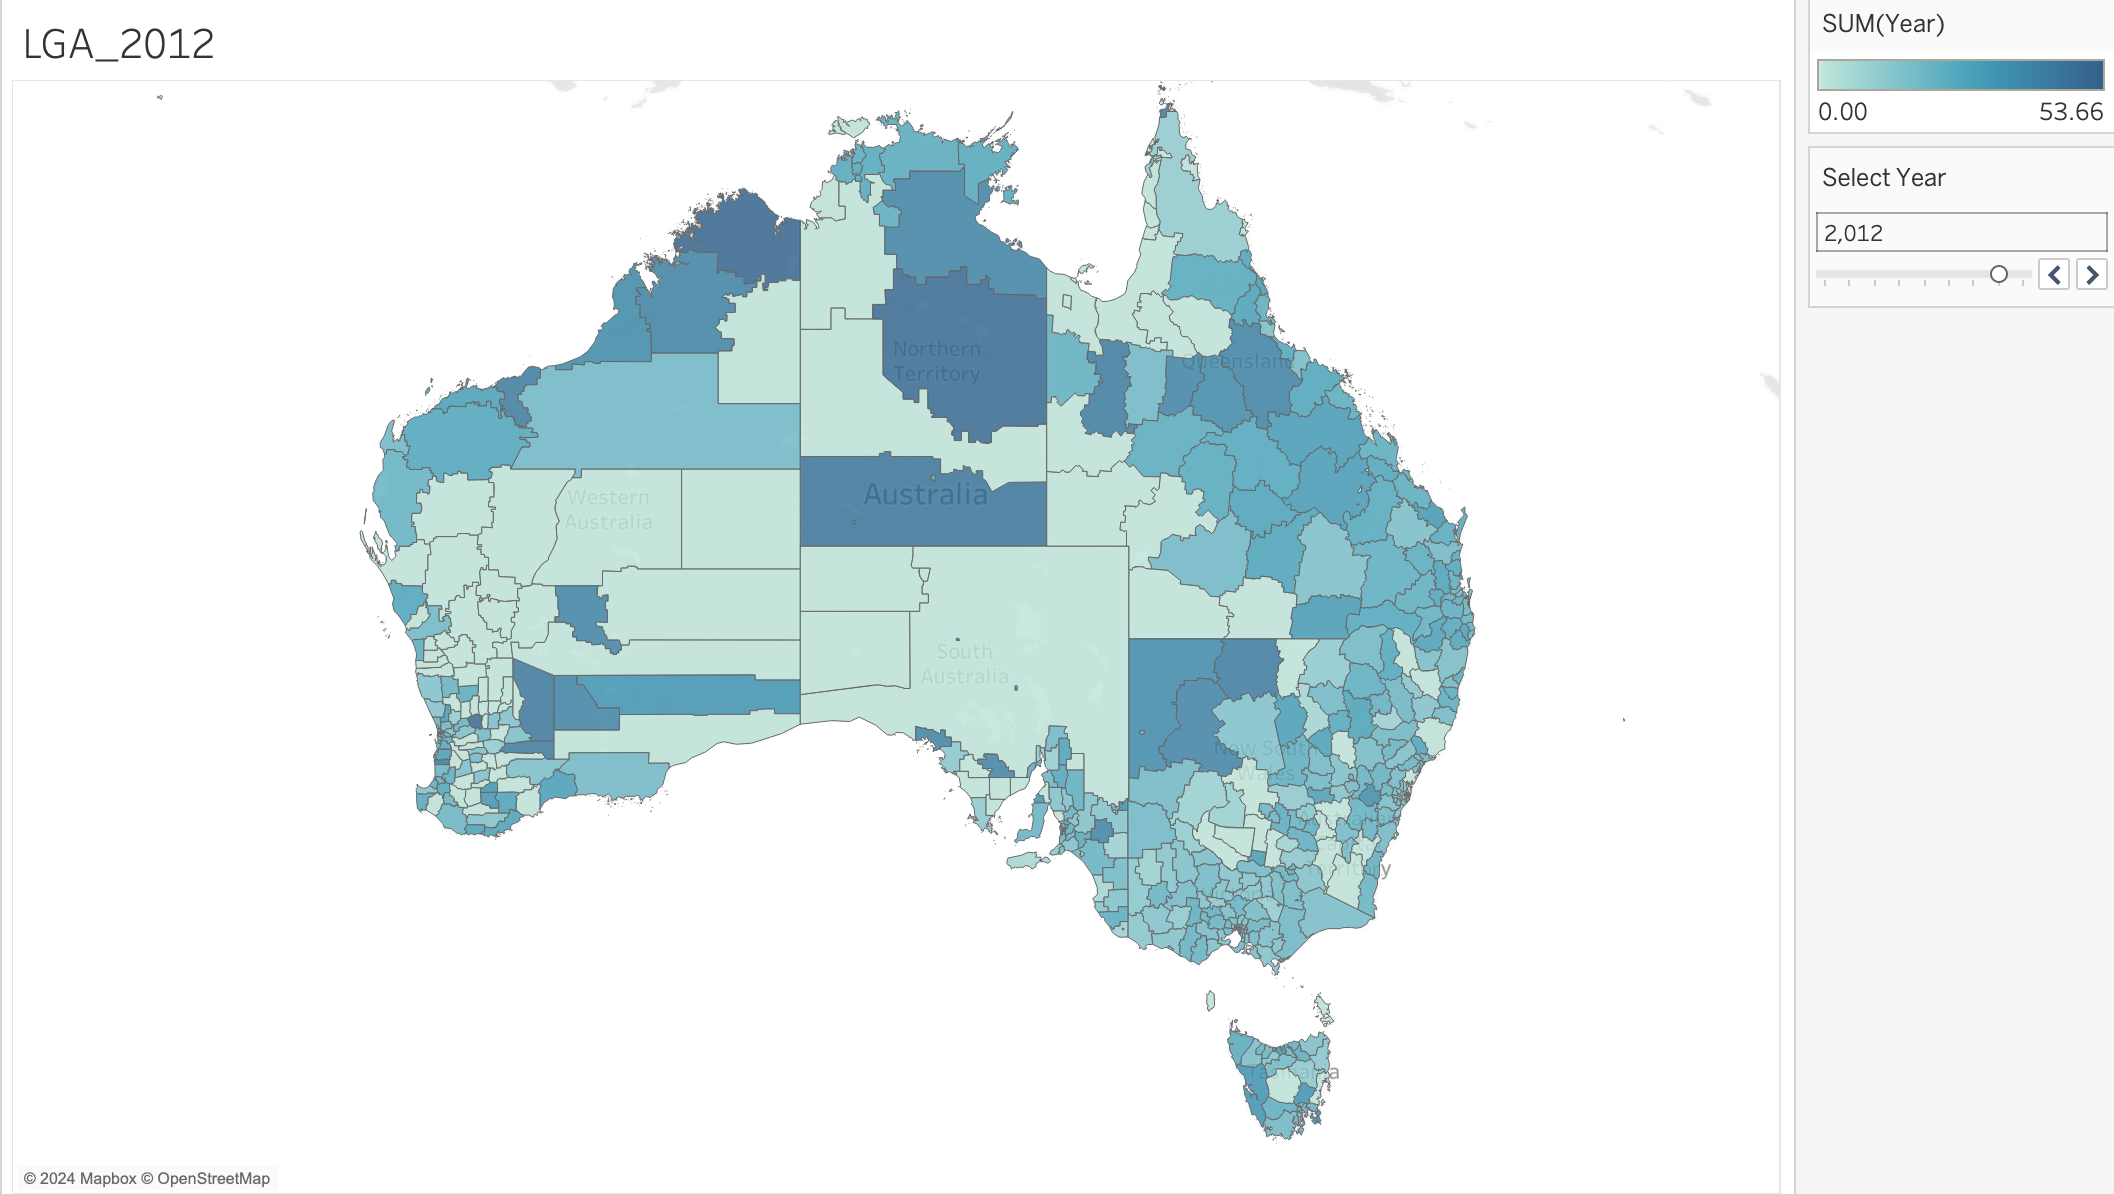
\includegraphics[width=0.45\textwidth]{images/Fig30.8.png}
        \label{fig:subfig17}
    }
    \vskip10pt
    \centering
    \subfloat[Heat map for 2013]{ % Manually manage the numbering
        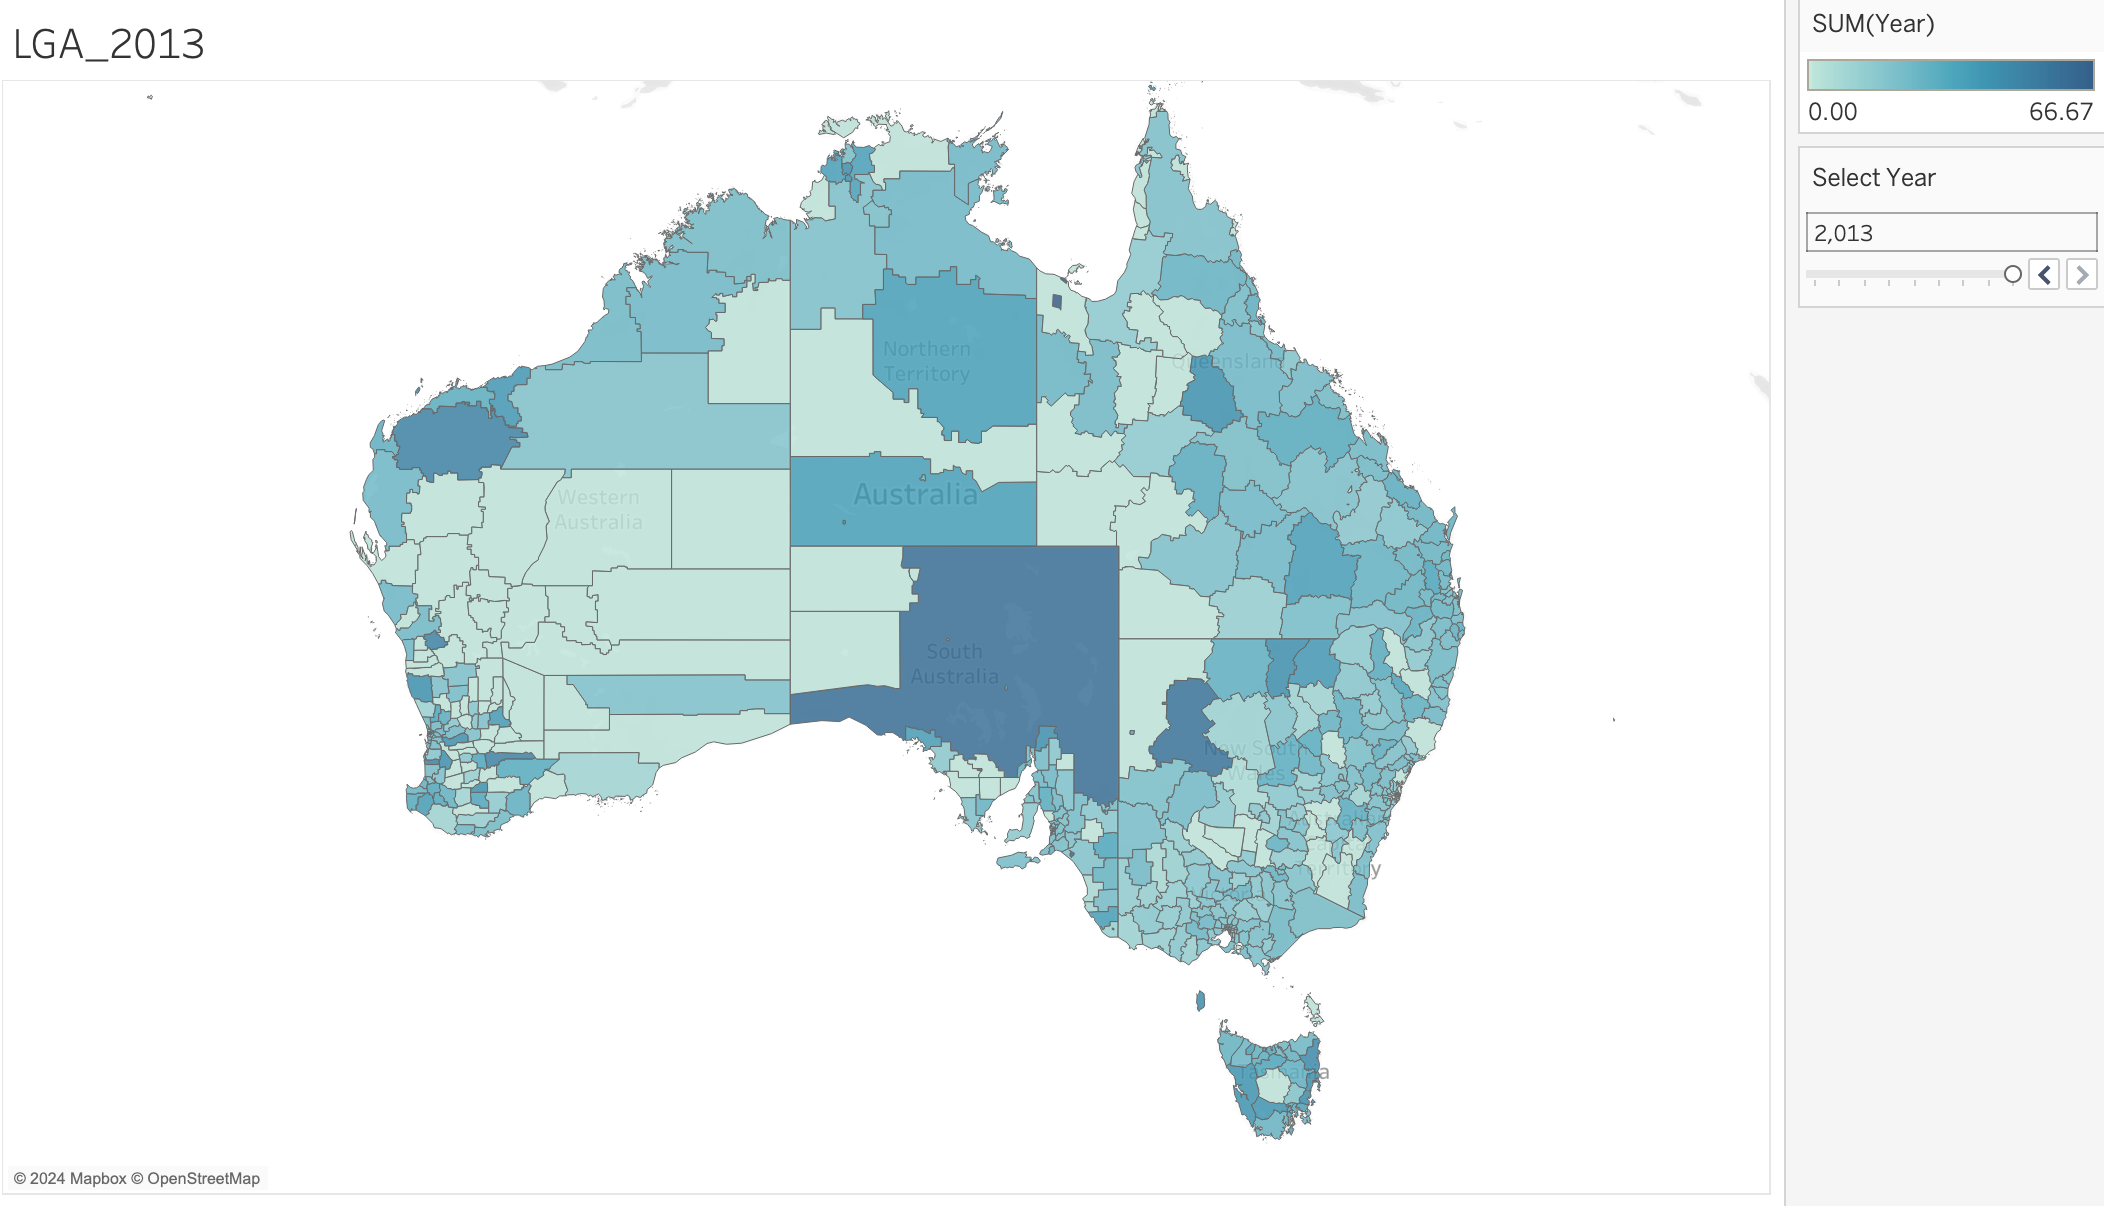
\includegraphics[width=0.45\textwidth]{images/Fig30.9.png}
        \label{fig:subfig18}
    }
    \centering
    \caption{Heat maps for LGA areas 2005 to 2013 (Part 2).}
    \label{fig:mainfigure4}
\end{figure*}
\clearpage



Key Observations and Insights: 
\begin{itemize} 
    \item Color Scheme: Darker teal shades represent higher attrition rates, while lighter shades indicate lower rates for the years 2007 to 2013 (Figures \ref{fig:mainfigure3} and \ref{fig:mainfigure4}).
    \item Regional Trends: Northern regions, particularly in Queensland, consistently show darker shades, reflecting higher attrition rates.
    \item Southern regions, including parts of New South Wales and Victoria, exhibit lighter shades, indicating lower attrition rates. Eastern coastal areas generally maintain moderate to low attrition rates, with some fluctuations across the years. Western areas also appear lighter, likely due to imputed minimum attrition rates where data was missing.
    \item Certain regions, such as Tasmania and parts of Western Australia, show increasing attrition rates over time, with noticeable darkening from 2007 to 2013. However, most central and southern areas exhibit stable trends with minor fluctuations.
    \item Heatmap Utility: The heatmaps effectively visualize the intensity of student attrition across regions, highlighting geographical and temporal patterns.
    \item Color Choice: Teal is chosen for its clarity and neutral tone, creating a strong visual contrast that emphasizes regional differences in attrition rates. The palette ensures that regions with minimal data or low attrition rates remain distinguishable from those with higher rates.
\end{itemize}
\begin{figure}[H]
    \centering
    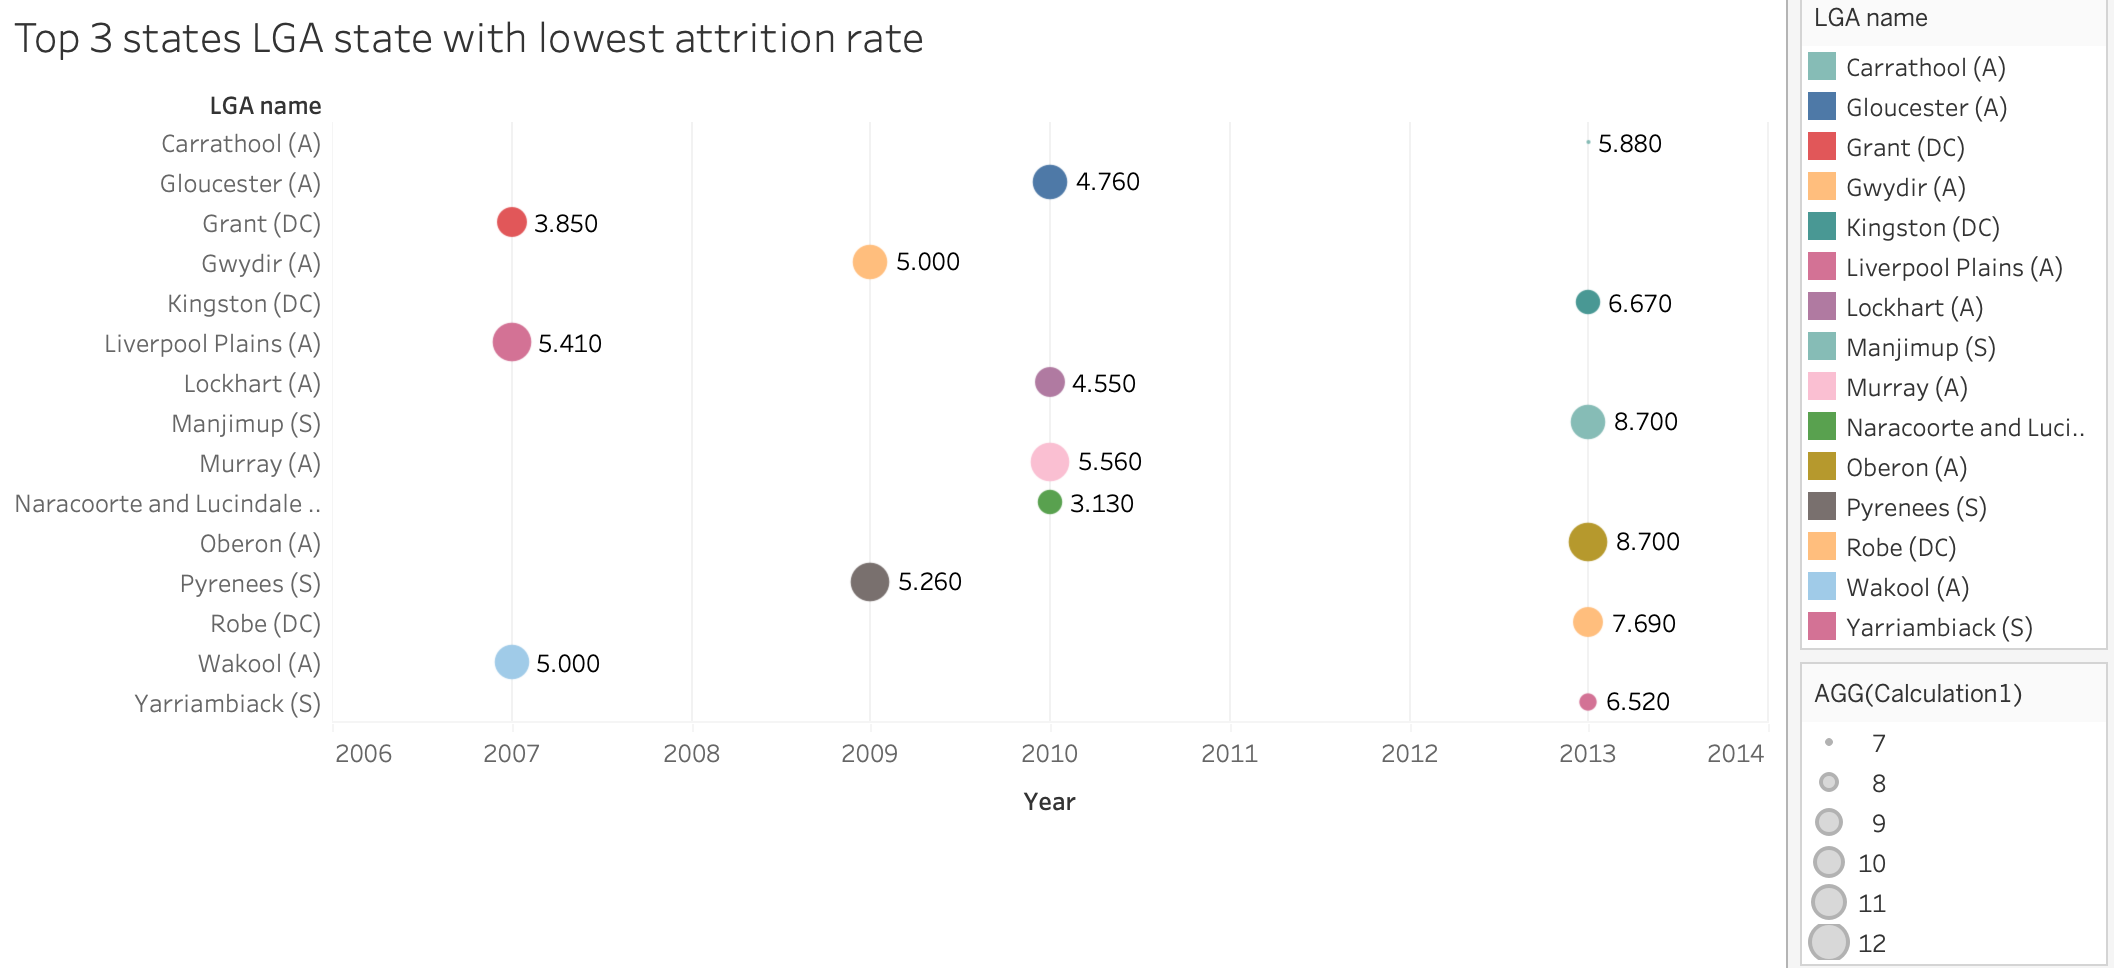
\includegraphics[width=0.4\textwidth]{images/Fig32.1.png}
    \caption{Scatter plot for top 3 states(based on LGA) with lowest attrition rate across years.}
    \label{fig:bubble3}
\end{figure}
\begin{figure}[H]
    \centering
    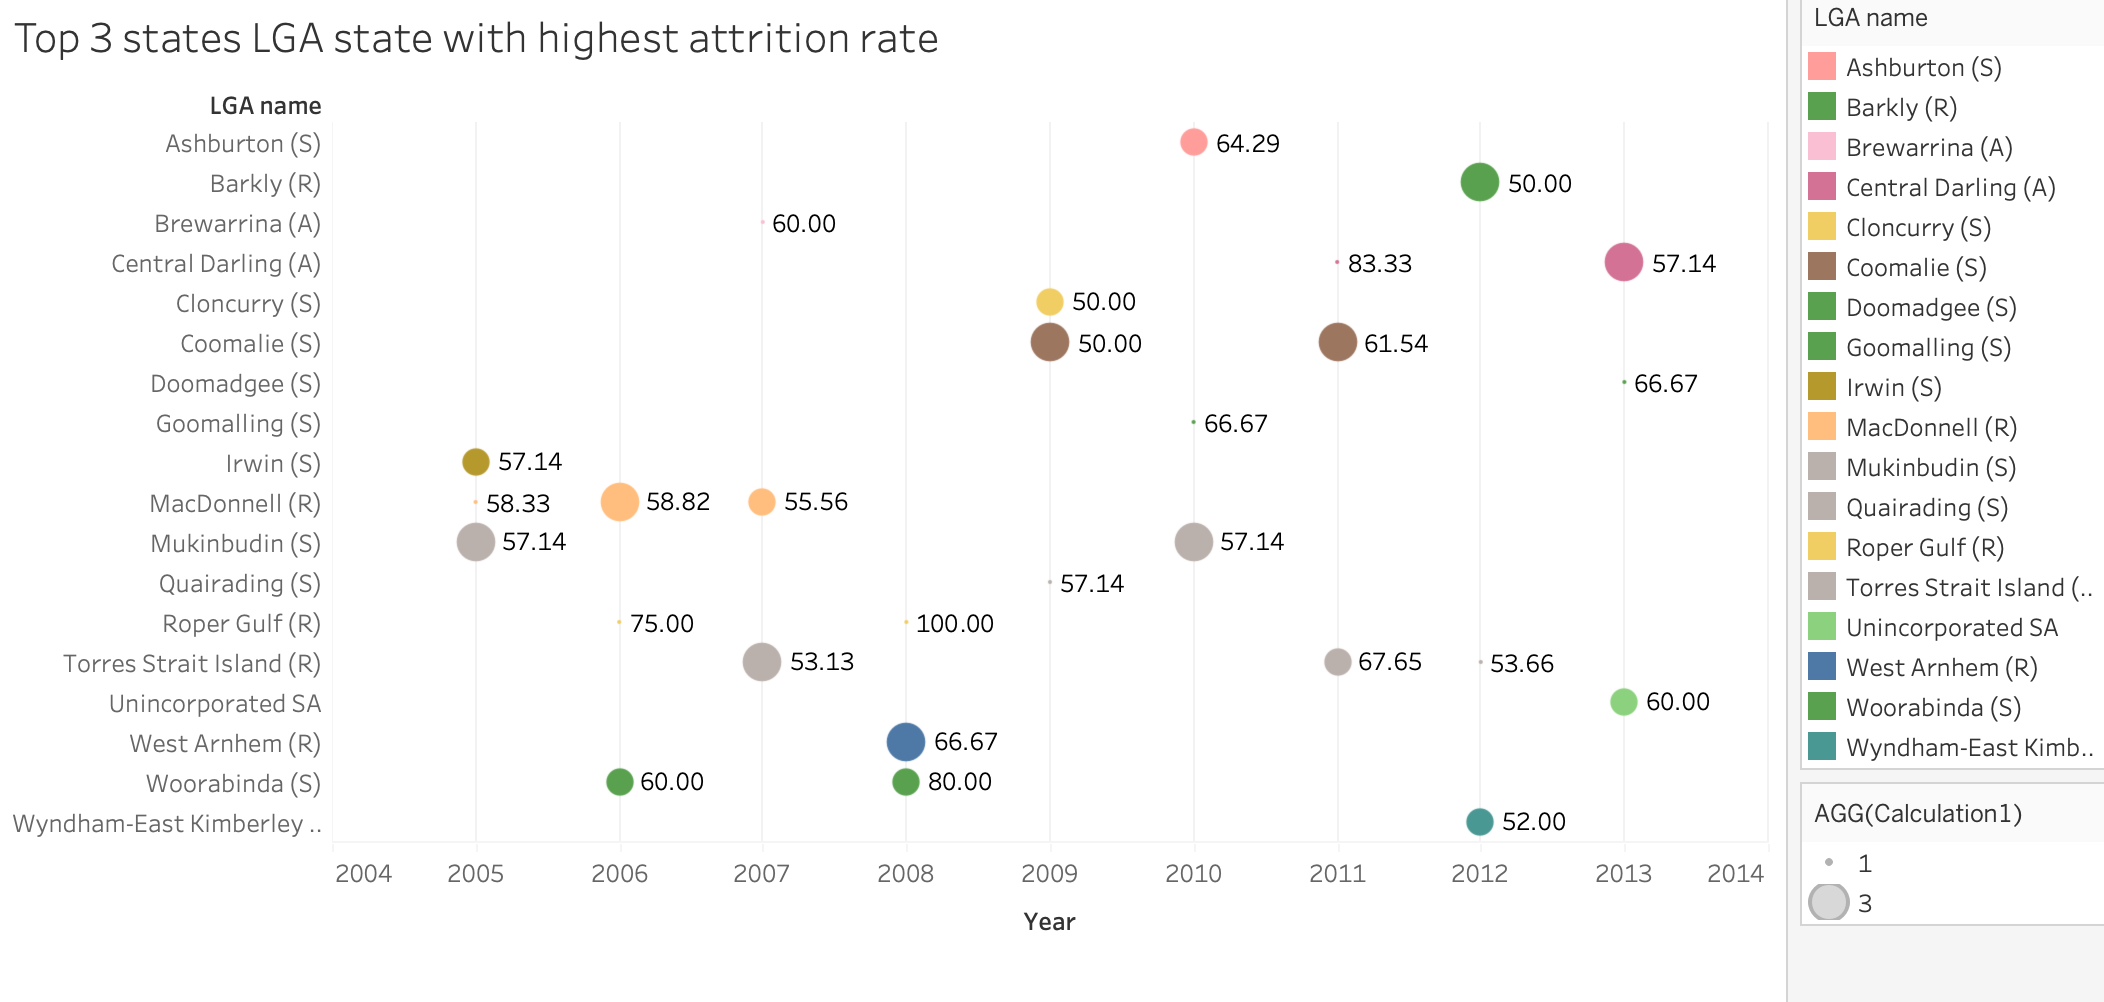
\includegraphics[width=0.4\textwidth]{images/Fig32.2.png}
    \caption{Scatter plot for top 3 states(based on LGA) with highest attrition rate across years.}
    \label{fig:bubble4}
\end{figure}

We have plotted bubble charts (Figures \ref{fig:bubble3} and \ref{fig:bubble4}) to visualize the top 3 states with the highest and lowest attrition rates across different years for LGA regions. Key observations and insights are:
\begin{itemize} 
    \item Figures \ref{fig:bubble3} and \ref{fig:bubble4} use circle size to represent attrition rates. In Figure \ref{fig:bubble3}, smaller circles indicate regions with the lowest attrition rates, and in Figure \ref{fig:bubble4} indicate regions with the highest attrition rates. 
    \item Figure \ref{fig:bubble3} shows the top 3 states with the lowest attrition rates across years. There is no consistent pattern across years. In 2013, the states with the lowest rates were Carathool (A) (5.88\%), followed by Yarriambiack (S) (6.52\%) and Kingston (DC) (6.67\%). 
    \item Figure \ref{fig:bubble4} displays the top 3 states with the highest attrition rates across years. There is some consistency with states such as MacDonnell (R) (light orange), Torres Strait Island, and Mukinbudin (S) (grey). In 2013, the states with the highest rates were Doomadgee (S) (66.67\%), followed by Unincorporated SA (60\%) and Central Darling (A) (57.14\%). 
    \item The bubble charts use inverse proportionality for circle size relative to attrition rates. This approach was chosen because direct proportionality resulted in circles that were too small to visualize effectively. 
\end{itemize}
\vspace{10pt}
\subsubsection{Comparision between LGA and SA3 area Analysis:} It is observed that LGA area provide more detail compared to SA3 areas,since LGA is distributed into more areas as compared to SA3 areas.
We have plotted heat map for average rate of change of attrition rate per year across different states according to SA3 (Figure: \ref{fig:heatmap1}) and LGA (Figure: \ref{fig:heatmap2}) areas.

\begin{figure}[H]
    \centering
    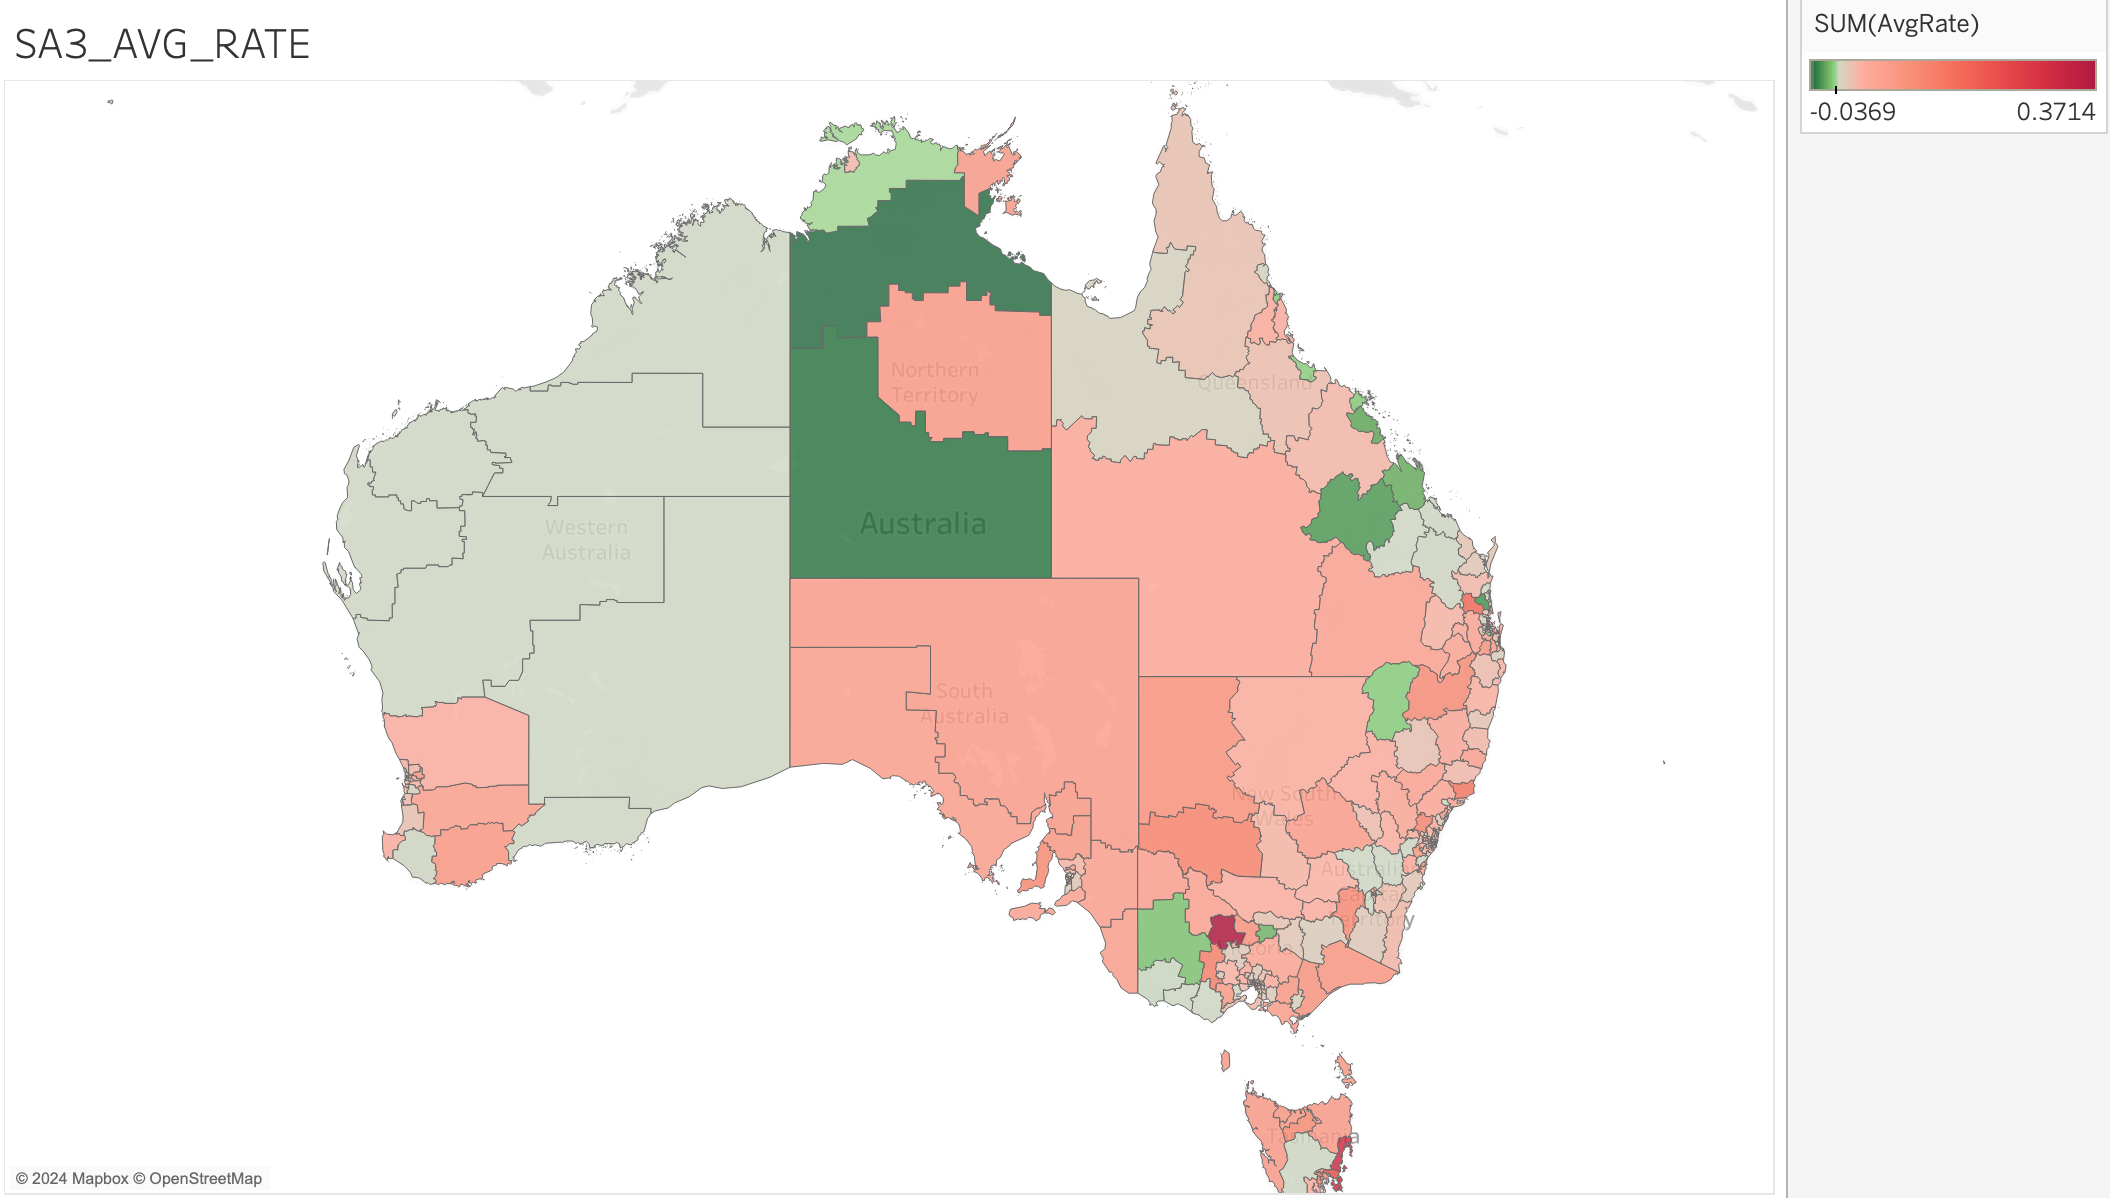
\includegraphics[width=0.4\textwidth]{images/Fig28.png}
    \caption{Heat map for average rate of change of attrition rate per year across different states according to SA3.}
    \label{fig:heatmap1}
\end{figure}
\begin{figure}[H]
    \centering
    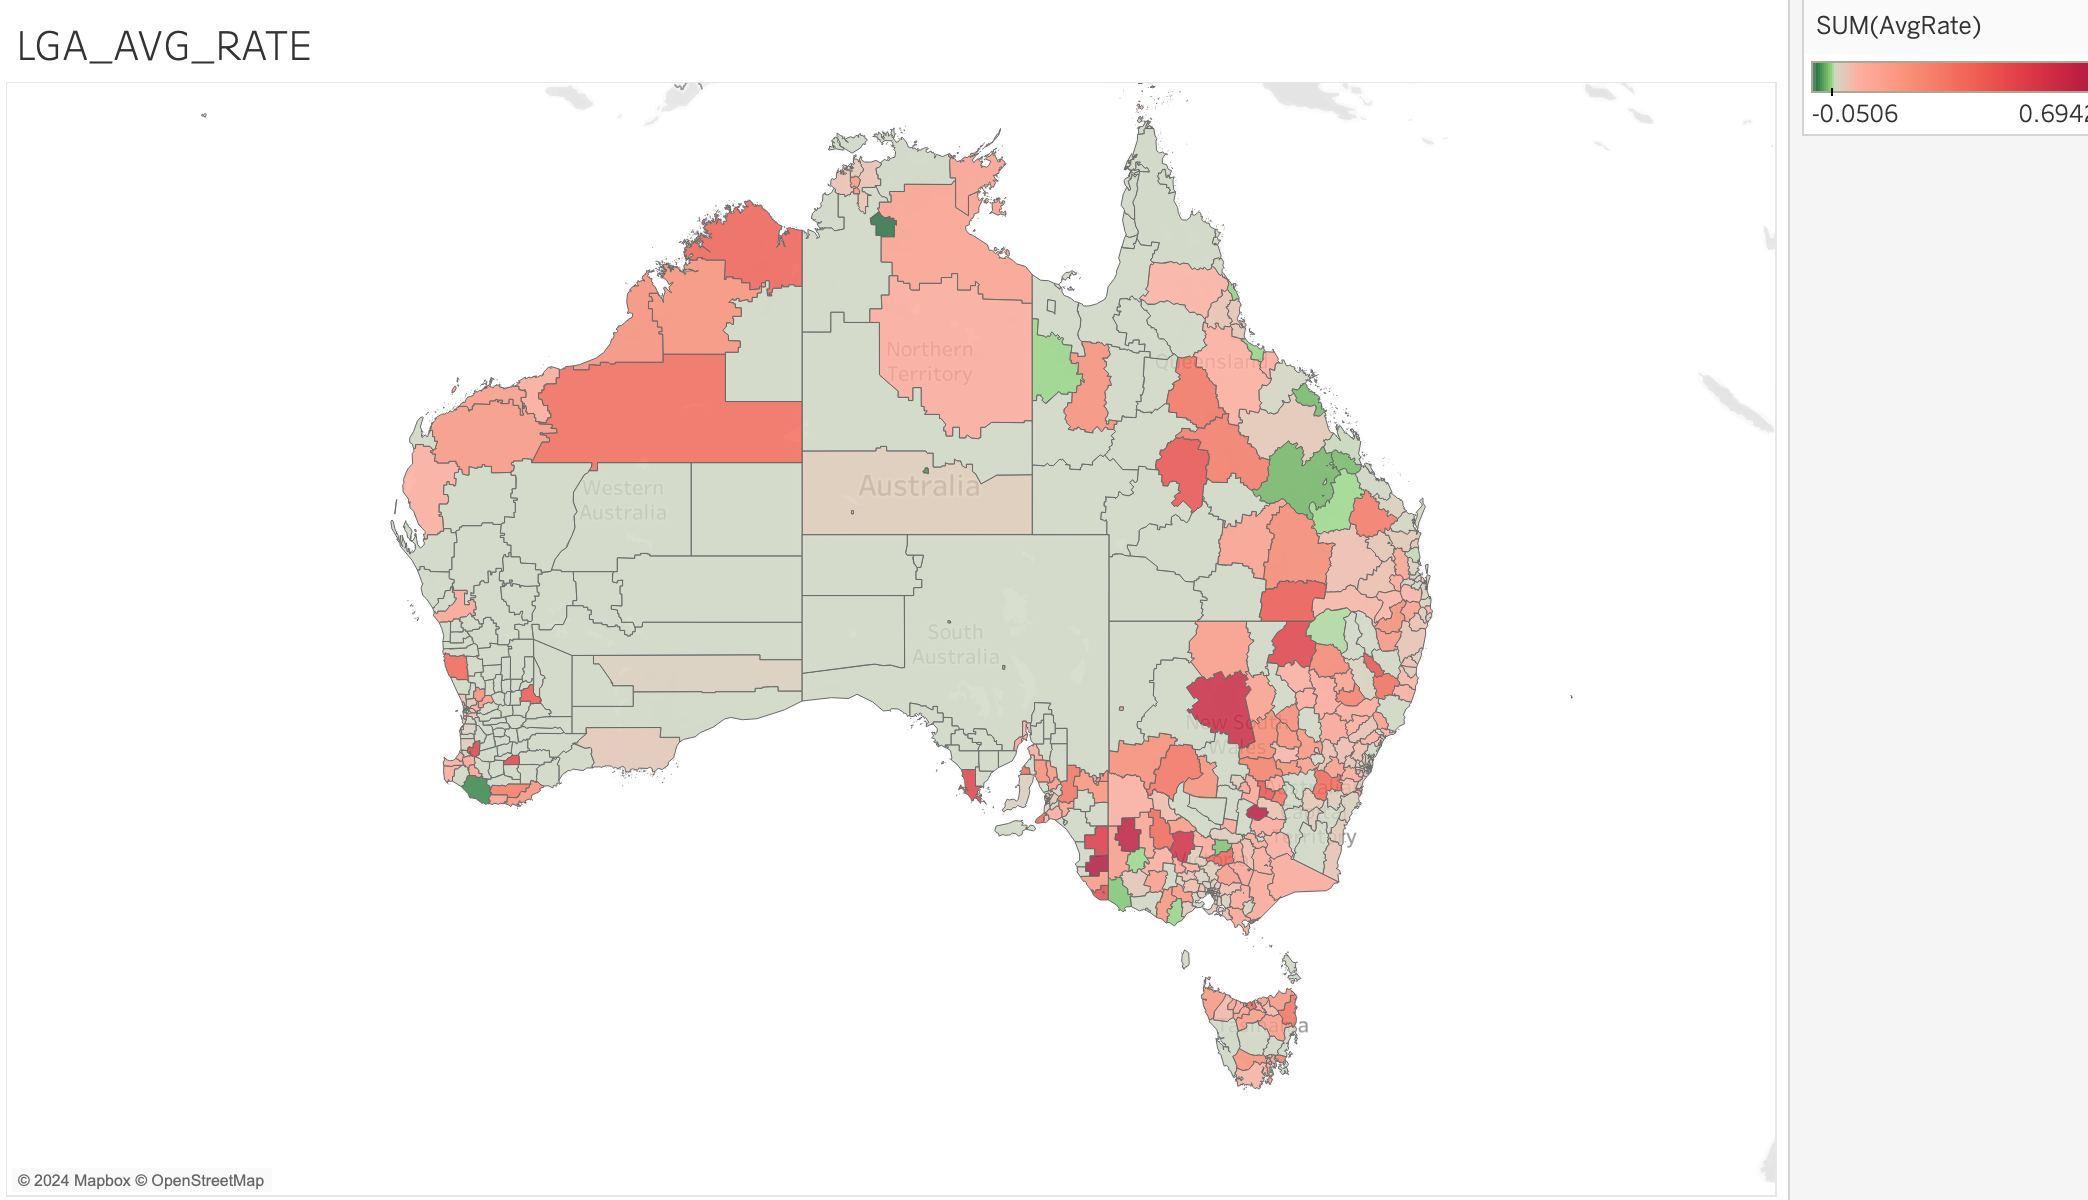
\includegraphics[width=0.4\textwidth]{images/Fig31.png}
    \caption{Heat map for average rate of change of attrition rate per year across different states according to LGA.}
    \label{fig:heatmap2}
\end{figure}
\clearpage
{Key observations and insights:}
\vspace{10pt}
\begin{itemize} 
    \item In Figures \ref{fig:heatmap1} and \ref{fig:heatmap2}, red represents a positive (increasing) average attrition rate, while green indicates a negative (decreasing) rate. Red highlights regions where the attrition rate is rising, signaling areas of concern, while green signifies declining rates, which is a positive trend for those regions.
    
    \item {Regional Trends:}
    \begin{itemize}
        \item In Figure \ref{fig:heatmap1}, many regions show a lighter red, indicating a slight increase in attrition, while northern, eastern, and southern areas show a green color, reflecting a slight decrease over time.
        \item Figure \ref{fig:heatmap2} shows that northern, southern, and eastern areas display a lighter shade of red, indicating a marginal increase in attrition.
    \end{itemize}
    
    \item Data Gaps: In both Figures \ref{fig:heatmap1} and \ref{fig:heatmap2}, the lightest green shades likely correspond to missing data or regions not available in the dataset.
    
    \item Insight: The overall trends suggest a mix of rising and falling attrition rates, with some regions benefiting from declining rates. These regions may offer potential areas for further investigation to understand factors contributing to these positive trends.
\end{itemize}

\text{Summary:}
Both heat maps show consistency with color variations. Red dominates in northern and eastern regions, indicating increasing attrition rates, while green areas in parts of the east reflect decreasing rates. The lightest green regions, especially in the west, likely represent missing data. These visualizations offer key insights into regions with both rising and falling attrition rates, which could guide targeted research and interventions.

\subsection{Summary: }
The analysis of attrition rates from 2005-2013 reveals several key trends. Overall attrition rates increased annually, with a notable exception in 2008, likely due to the Global Financial Crisis and improved student support systems. Age and gender differences were significant—students aged 25-39 had the lowest attrition, while those over 39 had the highest. Females had a higher overall attrition rate compared to males, with gender-based rates becoming more similar post-2008. Part-time students faced higher dropout rates than full-time students, and external study modes showed the highest attrition due to reduced engagement.

Attrition rates also varied across socio-economic backgrounds, with consistent rates for low-income students and a gradual increase for non-English-speaking and disabled students. Indigenous students showed improved retention, particularly after 2009. Additionally, students with higher ATAR scores consistently had lower attrition rates. The analysis highlights that factors like mode of study, socio-economic background, and academic preparedness strongly influence student attrition trends.

\section{Visualizations}
Following are the visualizations that are used and described
in detail in the section above.
\begin{enumerate}
    \item Bar plots
    \item Scatter Plots
    \item Pie Charts
    \item Bubble Chart
    \item Line Plots
    \item Area Plots
    \item Treemap
    \item Heatmap
    
\end{enumerate}

Also in each of the types wherever applicable, we have
employed various marks and channels for making the visualizations more expressive for someone to get the maximum
insights at the first glance.

\section {Member wise contributions}
As the sole team member, I independently handled all tasks for the project.
\par
All tasks were completed individually to ensure comprehensive coverage and cohesive results for the final project and report.
\end{document}

